\chapter{The Search for the Supersymmetric Top-quark}
\label{chap:search_stop}

\epigraph{
\textit{It will be remembered that the 18$^{th}$ century was, on the whole,
addicted to an ascending series of living forms shading by insensible degrees
into each other and leading onto man.
There was no consideration of the fact that this might be reading into Nature a greater
unity than she actually possessed. It led inevitably to some highly
questionable taxonomy produced in the effort to compress all life into positions upon a
single stairway.}
}
{
--Loren Eiseley, \textit{Darwin's Century}
}

\epigraph{
\textit{Cease, cows, life is short.}
}
{
--Gabriel Garc\'{i}a M\'{a}rquez, \textit{One Hundred Years of Solitude}
}

%%%%%%%%%%%%%%%%%%%%%%%%%%%%%%%%%%%%%%%%%%%%%%%%%%%%%%%%%%%%%%%%%%%%%%%%%%%%%%%%%%%%%%%%
%%%%%%%%%%%%%%%%%%%%%%%%%%%%%%%%%%%%%%%%%%%%%%%%%%%%%%%%%%%%%%%%%%%%%%%%%%%%%%%%%%%%%%%%
%%%%%%%%%%%%%%%%%%%%%%%%%%%%%%%%%%%%%%%%%%%%%%%%%%%%%%%%%%%%%%%%%%%%%%%%%%%%%%%%%%%%%%%%
%%%%%%%%%%%%%%%%%%%%%%%%%%%%%%%%%%%%%%%%%%%%%%%%%%%%%%%%%%%%%%%%%%%%%%%%%%%%%%%%%%%%%%%%

As described in Chapter~\ref{chap:bsm}, the lighter mass eigenstate of the superpartner of
the top quark, $\stopone$, plays an important role in helping solve the Hierarchy problem.
Most SUSY scenarios prefer \stopone masses not much larger than $1\,\TeV$, so as to keep them
at the scale EWSB.
If the \stopone exists, and is indeed lighter than the \TeV~scale, it may easily be produced in the $13\,\TeV$ $pp$ collisions
occurring at the LHC.
Searches for stops therefore play a prominent role in the searches for SUSY in ATLAS.

This chapter presents a search for the production of stop quarks.
The SUSY model considered here satisfies $R$-parity conservation, as do the majority of SUSY
searches at the LHC, which forces the \stopone to be produced in pairs and to follow
a decay chain ending in the stable LSP.
The LSP in these models is assumed to be the lightest neutralino, \ninoone.

SUSY searches performed in ATLAS are done using so-called `simplified models', wherein all parameters
of the MSSM are selected except for the masses of the sparticles relevant to the decays
of the sparticle being searched for.
For the case presented in this chapter, a search for \stopone is described and the simplified models
used to describe the SUSY signal process are parametrised by two free parameters: the mass of the 
\stopone and the mass of the \ninoone.
With these two parameters defined, the kinematics and production cross-section are fixed.
In the models considered, the \stopone is classified into three regions of phase space according
to the mass of the \ninoone, into which it decays.
The potential decays of the \stopone are illustrated by the decay diagrams in Figure~\ref{fig:stop_diagrams}.
showing the cases of the two-, three-, and four-body decays of the \stopone.
These decays are associated with three different regions of parameter space in the $(m_{\stopone}, m_{\ninoone})$ plane,
illustrated in Figure~\ref{fig:stop_boundaries}.
The analysis to be discussed in this chapter reports the results of a search for the production
of \stopone particles following the three-body decay, in which the mass-difference between the \stopone
and \ninoone, \sdiff, is less than (greater than) the mass of the SM top-quark ($W+b$ system).
This is the middle region of phase space indicated in Figure~\ref{fig:stop_boundaries}, $\stopone \rightarrow b W \ninoone$.
In this region, the two-body \stopone decays are kinematically suppressed and the \stopone decays via
an off-shell top-quark or \chinoonepm to the three-body $b W \ninoone$ final state.

\begin{figure}[!htb]
    \begin{center}
        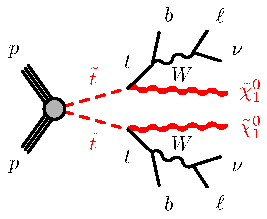
\includegraphics[width=0.3\textwidth]{figures/search_stop2l/signal/fgraph_stop_tN} \hspace{1cm}
        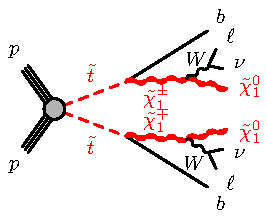
\includegraphics[width=0.3\textwidth]{figures/search_stop2l/signal/fgraph_stop_bCN} \\
        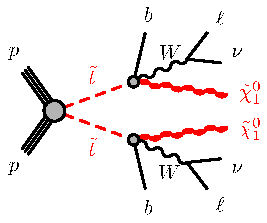
\includegraphics[width=0.3\textwidth]{figures/search_stop2l/signal/fgraph_3body} \hspace{1cm}
        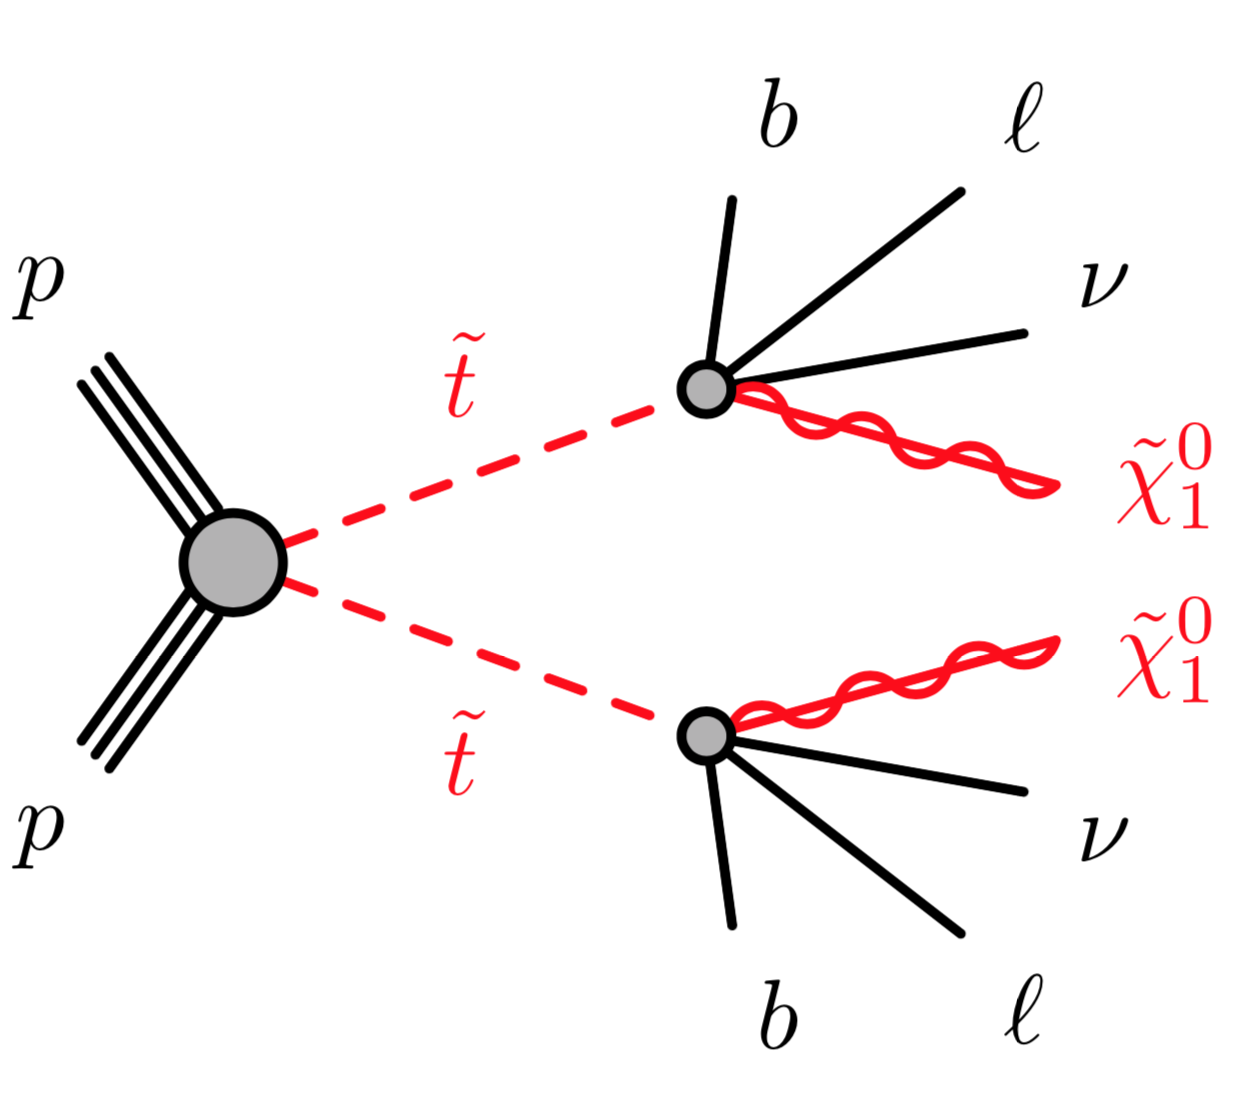
\includegraphics[width=0.3\textwidth]{figures/search_stop2l/signal/fgraph_stop_bffN}
        \caption{
            Decay diagrams for the \stopone relevant to the two-lepton final state of \stopone pair-production.
            \textit{\textbf{Top}}: Diagrams leading to the two-body decay of the \stopone, either
                into $\stopone \rightarrow t \ninoone$ (\textit{top left}) or $\stopone \rightarrow b \chinoonepm$ (\textit{top right}).
            \textit{\textbf{Bottom left}}: Three-body decay of the \stopone, $\stopone \rightarrow b W \ninoone$.
            \textit{\textbf{Bottom right}}: Four-body decay of the \stopone, $\stopone \rightarrow b f f^{\prime} \ninoone$.
        }
        \label{fig:stop_diagrams}
    \end{center}
\end{figure}

\begin{figure}[!htb]
    \begin{center}
        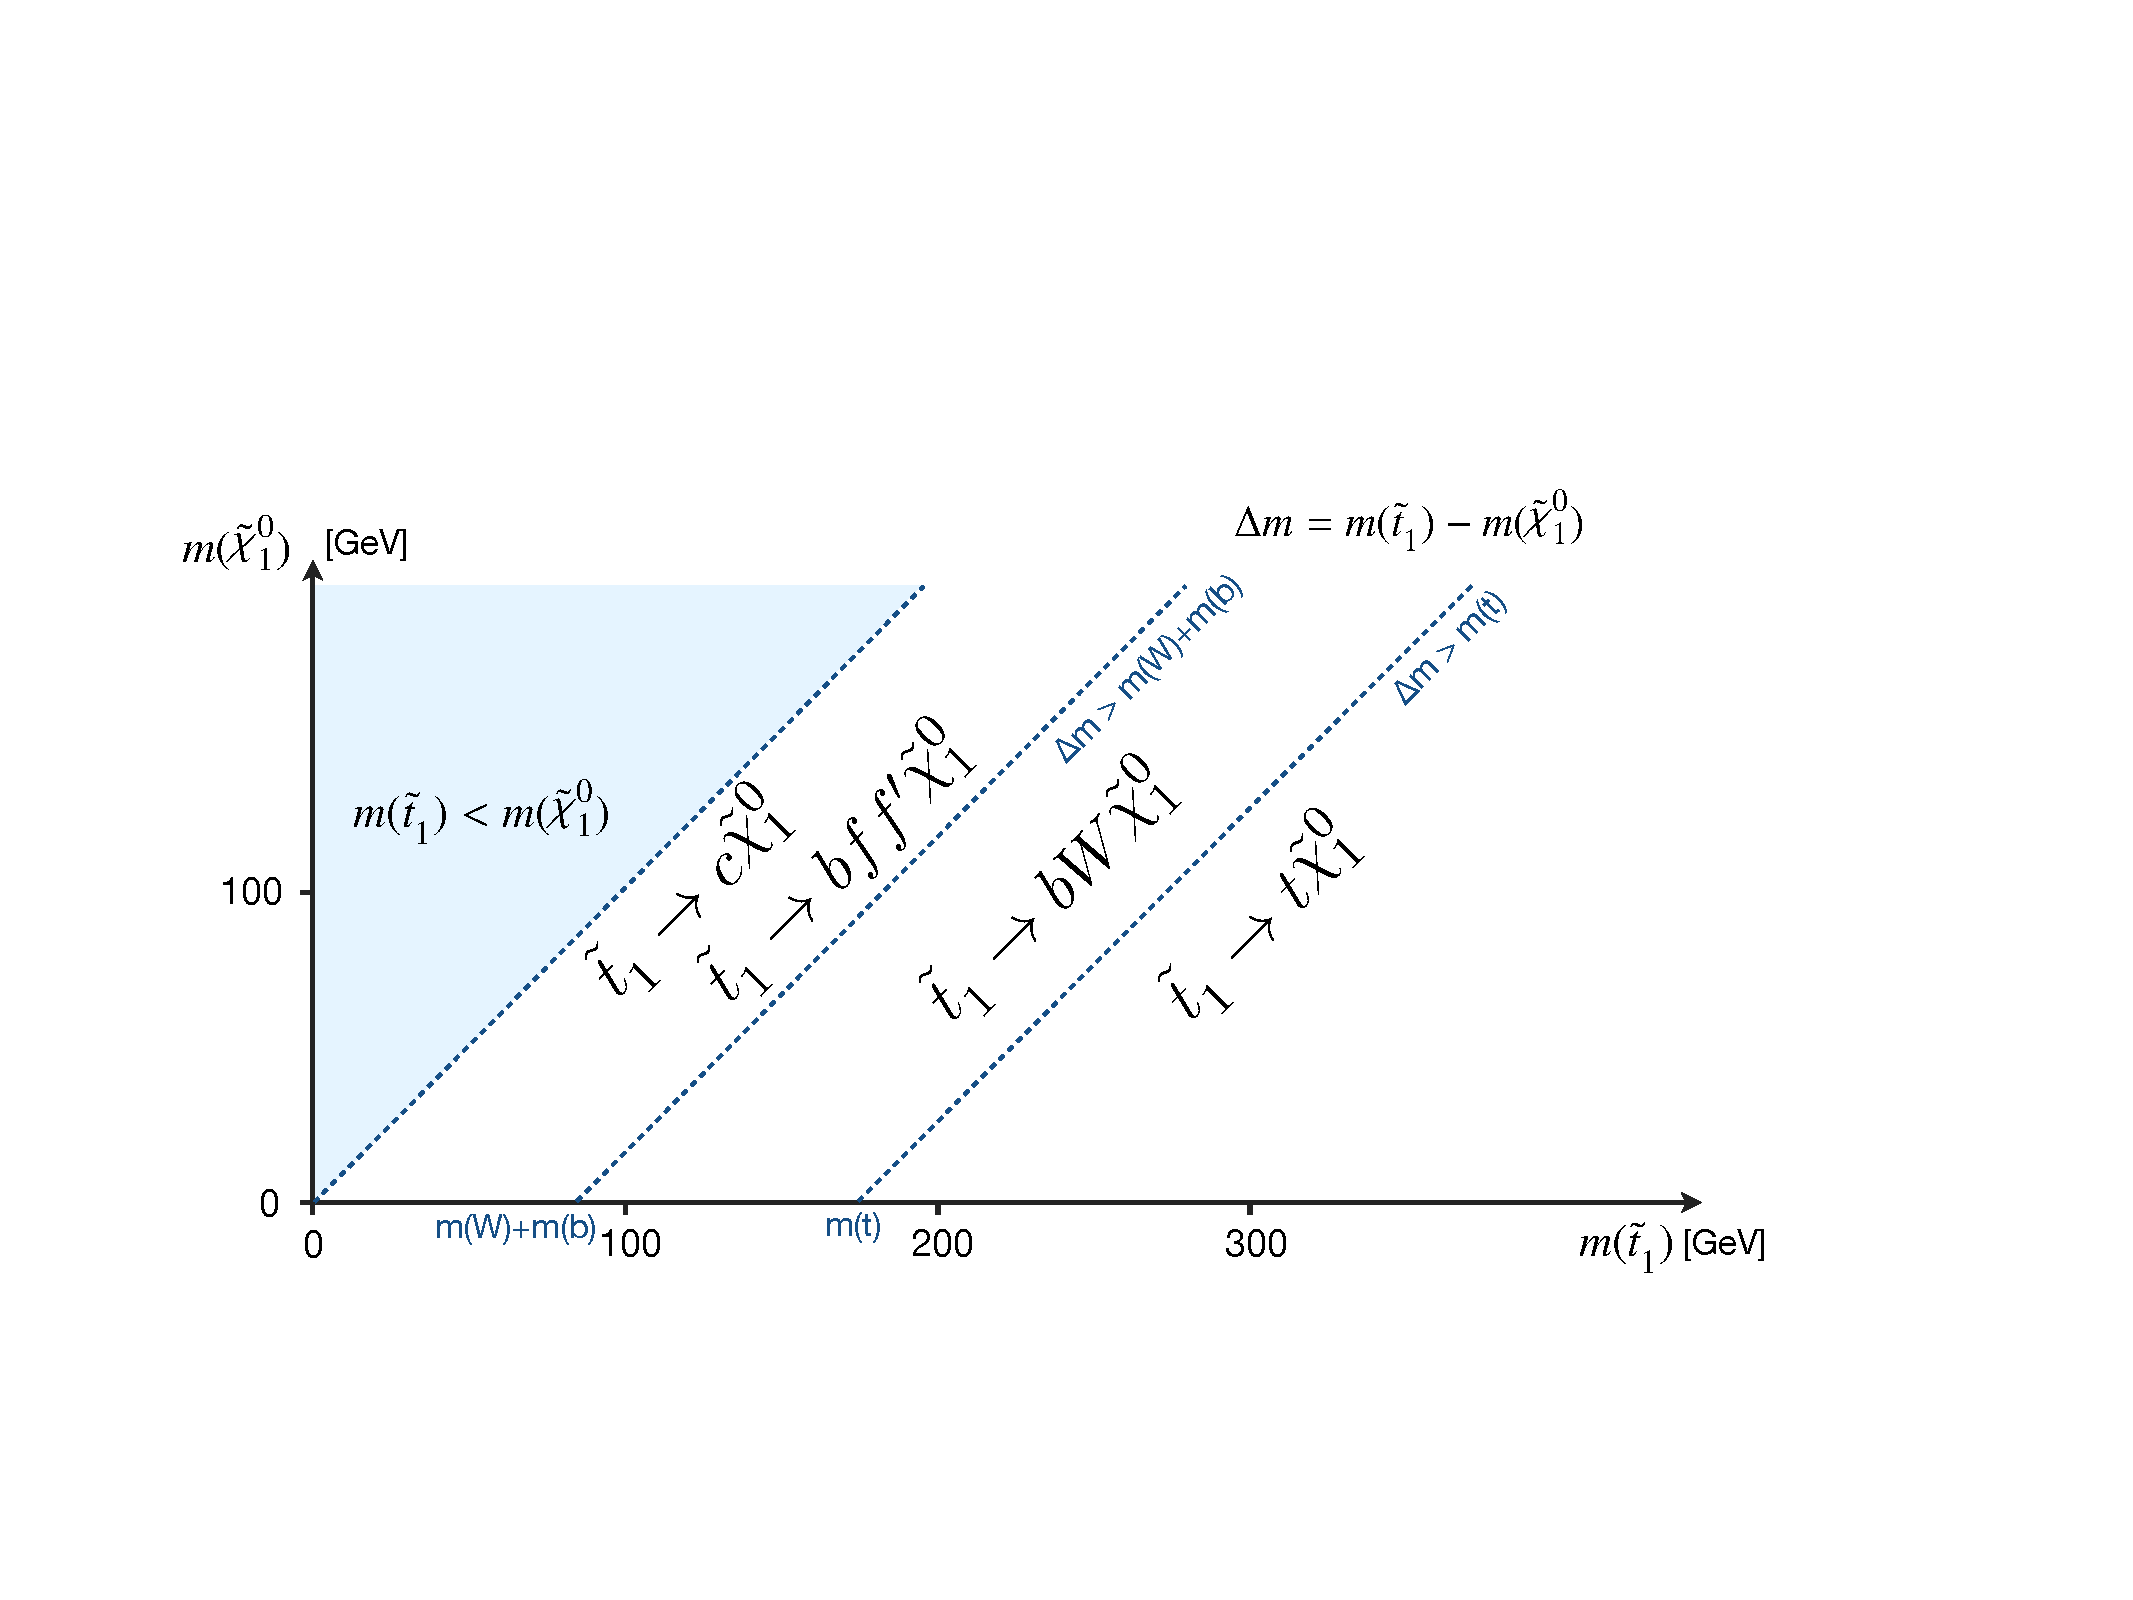
\includegraphics[width=0.7\textwidth]{figures/search_stop2l/signal/stop_LSP_boundaries}
        \caption{
            Kinematic boundaries in the (\stopone,\ninoone) plane, indicating the three kinematic
            regimes associated with the decay of the \stopone: the two-body $\stopone \rightarrow t \ninoone$
            decay ($\Delta m(\stopone, \ninoone) > m_t$), the three-body $\stopone \rightarrow b W \ninoone$ decay
            ($\Delta m(\stopone, \ninoone) < m_t$), and the four-body $\stopone \rightarrow b f f^{\prime} \ninoone$
            decay ($\Delta m(\stopone, \ninoone) < m_b + m_W$).
            Here $\Delta m(\stopone, \ninoone) = m_{\stopone} - m_{\ninoone}$.
        }
        \label{fig:stop_boundaries}
    \end{center}
\end{figure}

Figure~\ref{fig:run1_stop_summary} shows the results of the searches for \stopone particles performed
in Run 1 of the LHC by the ATLAS experiment.
This figure indicates the regions of SUSY parameter space, under the hypothesis of the
simplified model parametrised by the masses of the \stopone and \ninoone particles,
that are excluded at 95\% CL by the zero, one, and two lepton analyses.
It can be seen that the Run 1 analyses targeting the two-lepton final states did not effectively
cover the three-body regime, at least in comparison to all analyses in the two-body and four-body regions
of the $(m_{\stopone}, m_{\ninoone})$-plane.

Section~\ref{sec:susy_exclusion_plots} provides a brief introduction to the type of plots
shown in Figure~\ref{fig:run1_stop_summary}, which are the general SUSY exclusion plots
that are presented to summarise the results of SUSY searches based on simplified models
by both the ATLAS and CMS experiments.
Section~\ref{sec:stop_pheno} then begins by describing the kinematics and phenomenology of the three-body \stopone
decays that are being targeted in the SUSY analysis presented in this chapter.
With the signal kinematics in mind, Section~\ref{sec:stop_event_sel} describes the overall event
selection and object definition used in the analysis, so that the analysis' event sample can be understood.
Section~\ref{sec:stop_strategy} describes how the phenomenology described in Section~\ref{sec:stop_pheno}
motivates a particular choice of discriminating observables that are sensitive to the three-body decay
of the \stopone particle, as well as the definition of the analysis' SRs.
Section~\ref{sec:stop_background_estimate} describes the analysis' background estimation
strategy, particular the definition of CRs and VRs used to constrain the dominant
SM backgrounds.
Section~\ref{sec:stop_results} closes the chapter with the results of the search for
the three-body \stopone in the two-lepton final state.


\begin{figure}[!htb]
    \begin{center}
        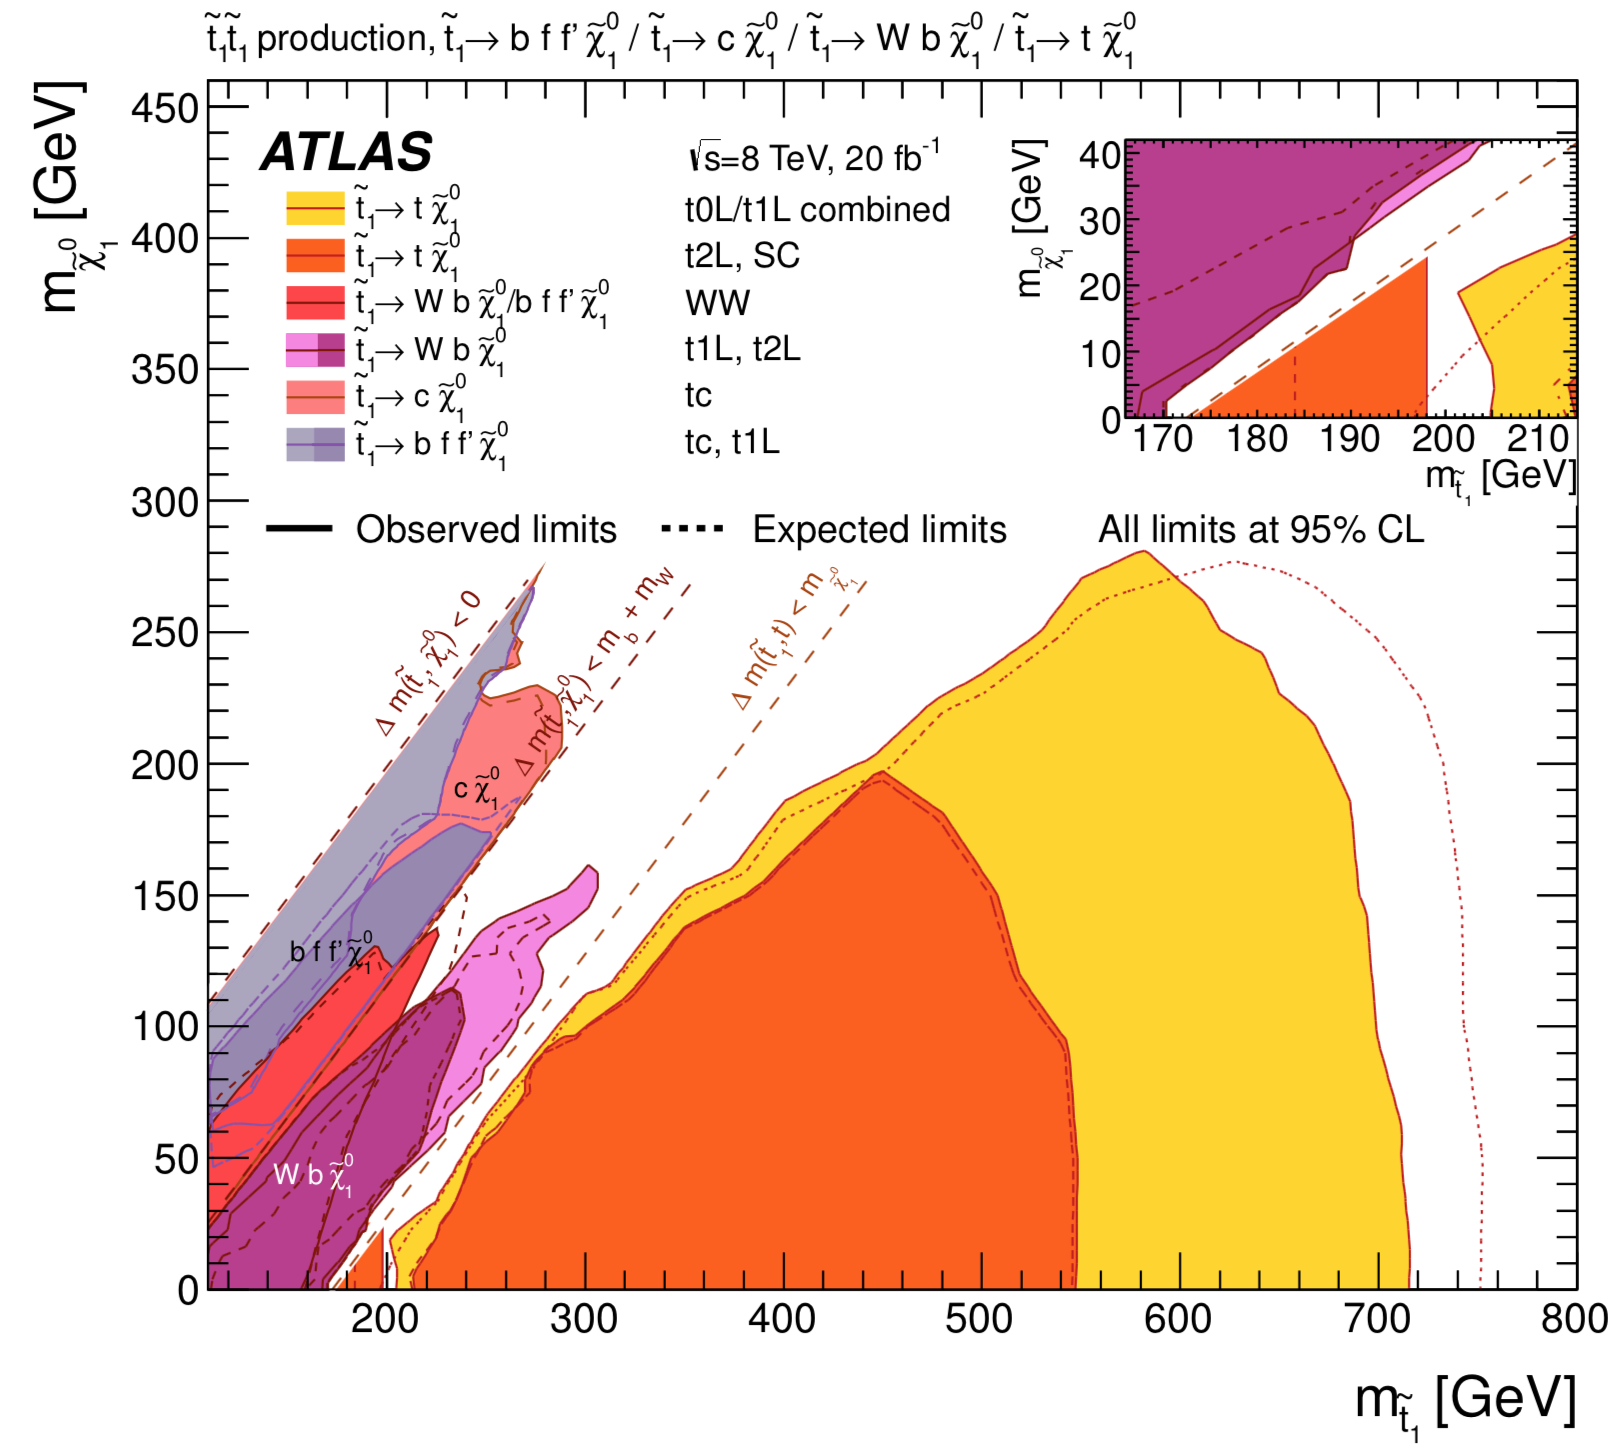
\includegraphics[width=0.7\textwidth]{figures/search_stop2l/run1_stop_summary}
        \caption{
            Summary of SUSY \stopone searches in the (\stopone, \ninoone) plane
            at the end of Run 1.
            The searches relevant to the work in the present thesis are indicated by the 
            coverage of purple and dark orange: `t1L,t2L' and `WW', respectively.
            Figure taken from Ref.~\cite{StopRun1Summary}.
        }
        \label{fig:run1_stop_summary}
    \end{center}
\end{figure}

\FloatBarrier
\section{Aside: SUSY Exclusion Plots}
\label{sec:susy_exclusion_plots}

In this section we describe the typical SUSY exclusion plot, illustrated in Figure~\ref{fig:susy_exclusion_cartoon}.
These plots are used when presenting the results of SUSY searches based on the assumptions
made in simplified models of the MSSM, parametrised only by the masses of the
pair-produced sparticle and the stable sparticle appearing in the final state (the LSP), assuming $R$-parity
conservation. The main things to observe in this plot are as follows:

\begin{enumerate}
    \item The region contained \textit{within} the contours is the region of SUSY parameter space,
        under the assumption of the simplified model, excluded at 95\% CL
    \item The region in which the mass of the produced
        sparticle is less than the mass of the LSP is kinematically forbidden
    \item The analysis sensitivity (i.e. power to exclude) decreases as the mass of the produced sparticle increases
    \item The analysis sensitivity (i.e. power to exclude) decreases as $\sdiff \rightarrow 0$ ($\sdiff \rightarrow m_X$,
        with $m_X$ a mass scale related to an intermediate state appearing in the sparticle decay)
    \item The expected 95\% CL exclusion limits are reported with their $\pm 1 \sigma$ uncertainty band,
        related to the precision of the analyses based on their systematic uncertainty evaluation
    \item The observed 95\% CL exclusion limit is not reported with an error
\end{enumerate}

Item (3) in the above is related to the fact that the cross-section of the SUSY sparticle production cross-section
is a function of only the mass of the pair-produced sparticle in the simplified models assumed here.
The production cross-section decreases in proportion to the mass of the sparticle, indicated in Figure~\ref{fig:susy_xsec},
which leads to analyses becoming less sensitive to the scenarios with larger masses of the produced sparticles.

Item (4) is also relatively straightforward.
As the masses of the produced sparticle and final-state LSP become nearer to one another, and even
degenerate, kinematic phase space suppression results in there being less energy-momentum available to be transferred to the final state
particles.
This results in final state particles having typically lower energies and momenta,
making them difficult to trigger on and reconstruct efficiently.
This inefficiency reduces an analysis' sensitivity to these kinematic regimes, since the final states become experimentally
inaccessible.
This scenario also appears when the produced sparticle follows a more complex decay chain,
as in the cases illustrated in Figure~\ref{fig:stop_diagrams}, where intermediate mass scales such as the
mass of the SM top-quark or $W$-boson are introduced.
Near these regions, the kinematics of the particles decaying from the objects defining these intermediate
mass scales change rapidly.
As a result, analyses targeting particle kinematics on one side of such a boundary
cannot simultaneously be sensitive to the particle kinematics on the opposing side of the boundary.
For this reason, it is common practice to define separate analyses targeting each side of a given boundary,
as indicated in Figure~\ref{fig:run1_stop_summary}.

The expected limits in Item (5) in the above are related to running the analysis' hypothesis tests
on the SUSY scenarios indicated by the position on the $(m_{\stopone}, m_{\ninoone})$-plane,
and using for $\bm{N^{\text{obs}}}$ (c.f. Equations~\ref{eq:likelihood_main} and \ref{eq:full_likelihood}) the value in the SRs for the predicted background; that is, the
observed data counts in the analysis' signal regions are substituted with the value of the total predicted
background in the signal regions.
The observed data is still used in the CRs, which provide the normalisation correction factors as described in Section~\ref{sec:likelihood}.
The observed limits discussed in Item (6), on the other hand, take as $\bm{N^{\text{obs}}}$ the actual observed data counts
in the analysis' SRs.
Due to statistical fluctuations in the observed data, the expected and observed 95\%CL exclusion contours
do not typically overlap perfectly.

\begin{figure}[!htb]
    \begin{center}
        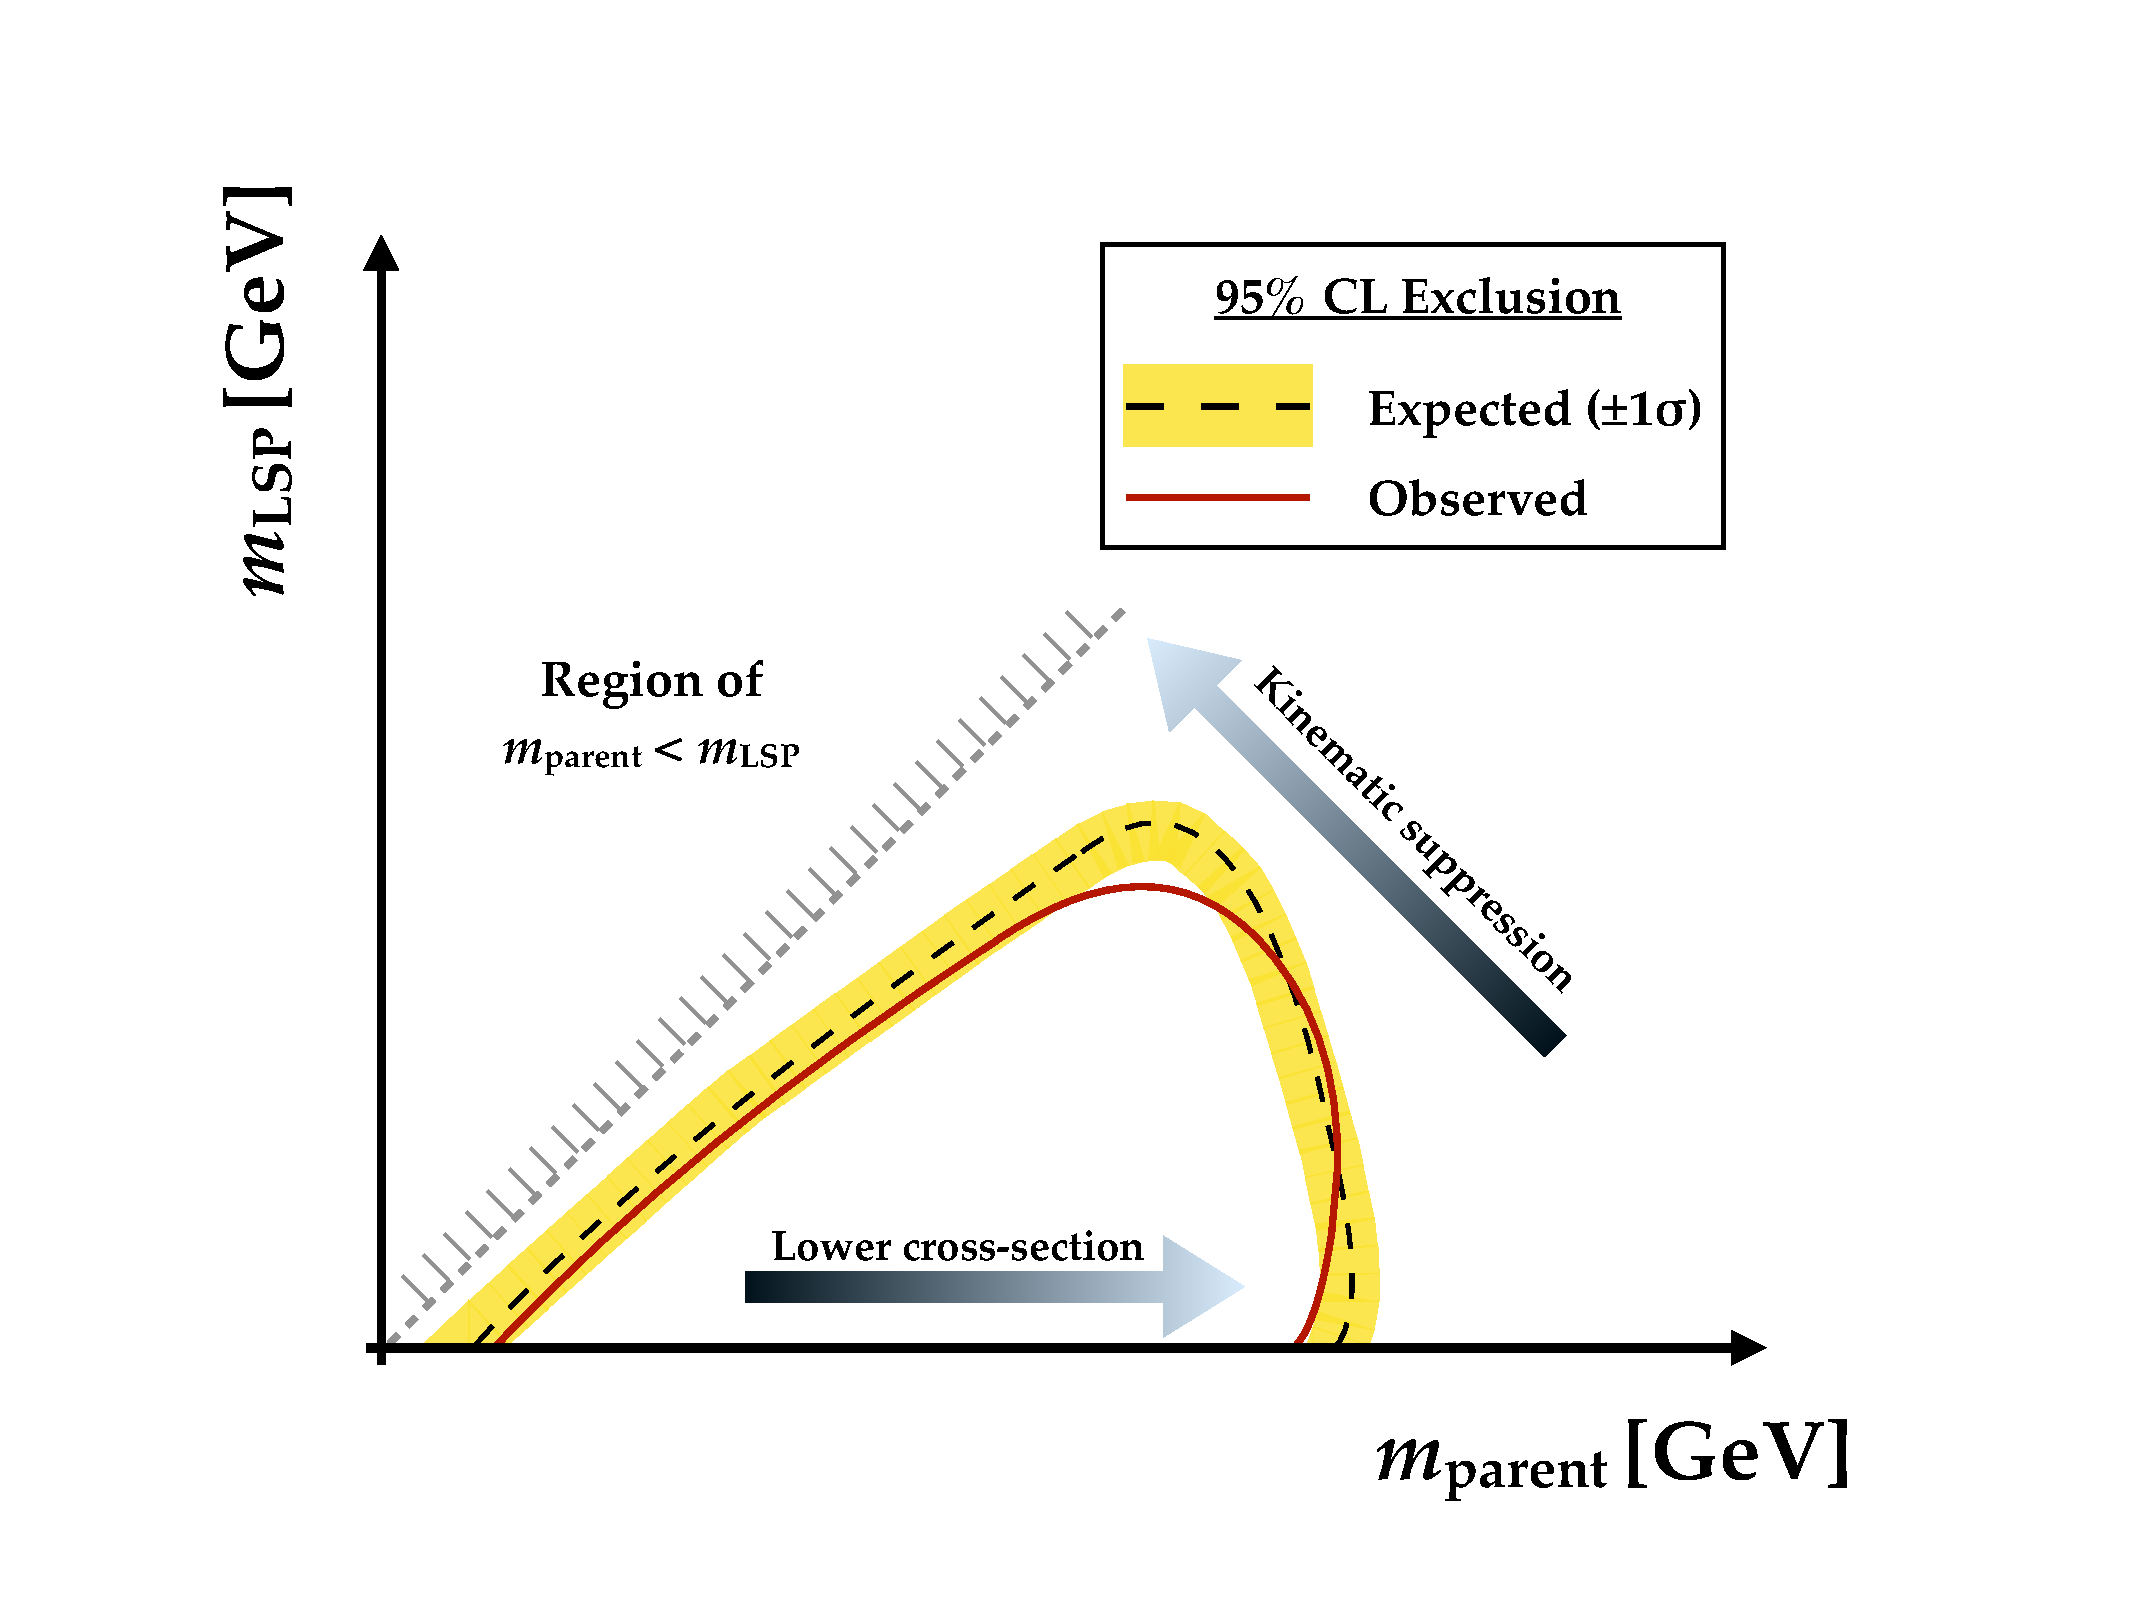
\includegraphics[width=0.8\textwidth]{figures/search_stop2l/susy_exclusion_cartoonPDF}
        \caption{
            Cartoon illustrating an example of a typical two-dimensional exclusion plot
            for a SUSY simplified model.
            The mass of the pair-produced SUSY particle is on the $x$-axis and the mass of the
            LSP to which it decays is on the $y$-axis.
            The region bounded by (i.e. inside of) the dashed-black (red) curves indicate
            the expected (observed) region of SUSY parameter space excluded at the 95\% CL.
            The $\pm 1\sigma$ error band is shown on the expected limits, and is based on the
            systematic uncertainties included in the analysis.
            SUSY exclusion curves such as these usually exhibit a triangular shape as a result
            of two competing effects, indicated by the arrows: 1) the reduction in production
            cross-section as the mass of the produced SUSY particle increases, and 2) kinematic
            suppression occurring when the phase space available to the final state decreases
            as a result of $\Delta m (x, y) = m_x - m_y \rightarrow 0$.
            Kinematic suppression results in the final state objects, such as leptons and $b$-tagged jets
            in the case presented in the current thesis,
            having very little momenta, thereby making it difficult to efficiently identify
            the event as being consistent with the given SUSY hypothesis being searched for.
        }
        \label{fig:susy_exclusion_cartoon}
    \end{center}
\end{figure}

\begin{figure}[!htb]
    \begin{center}
        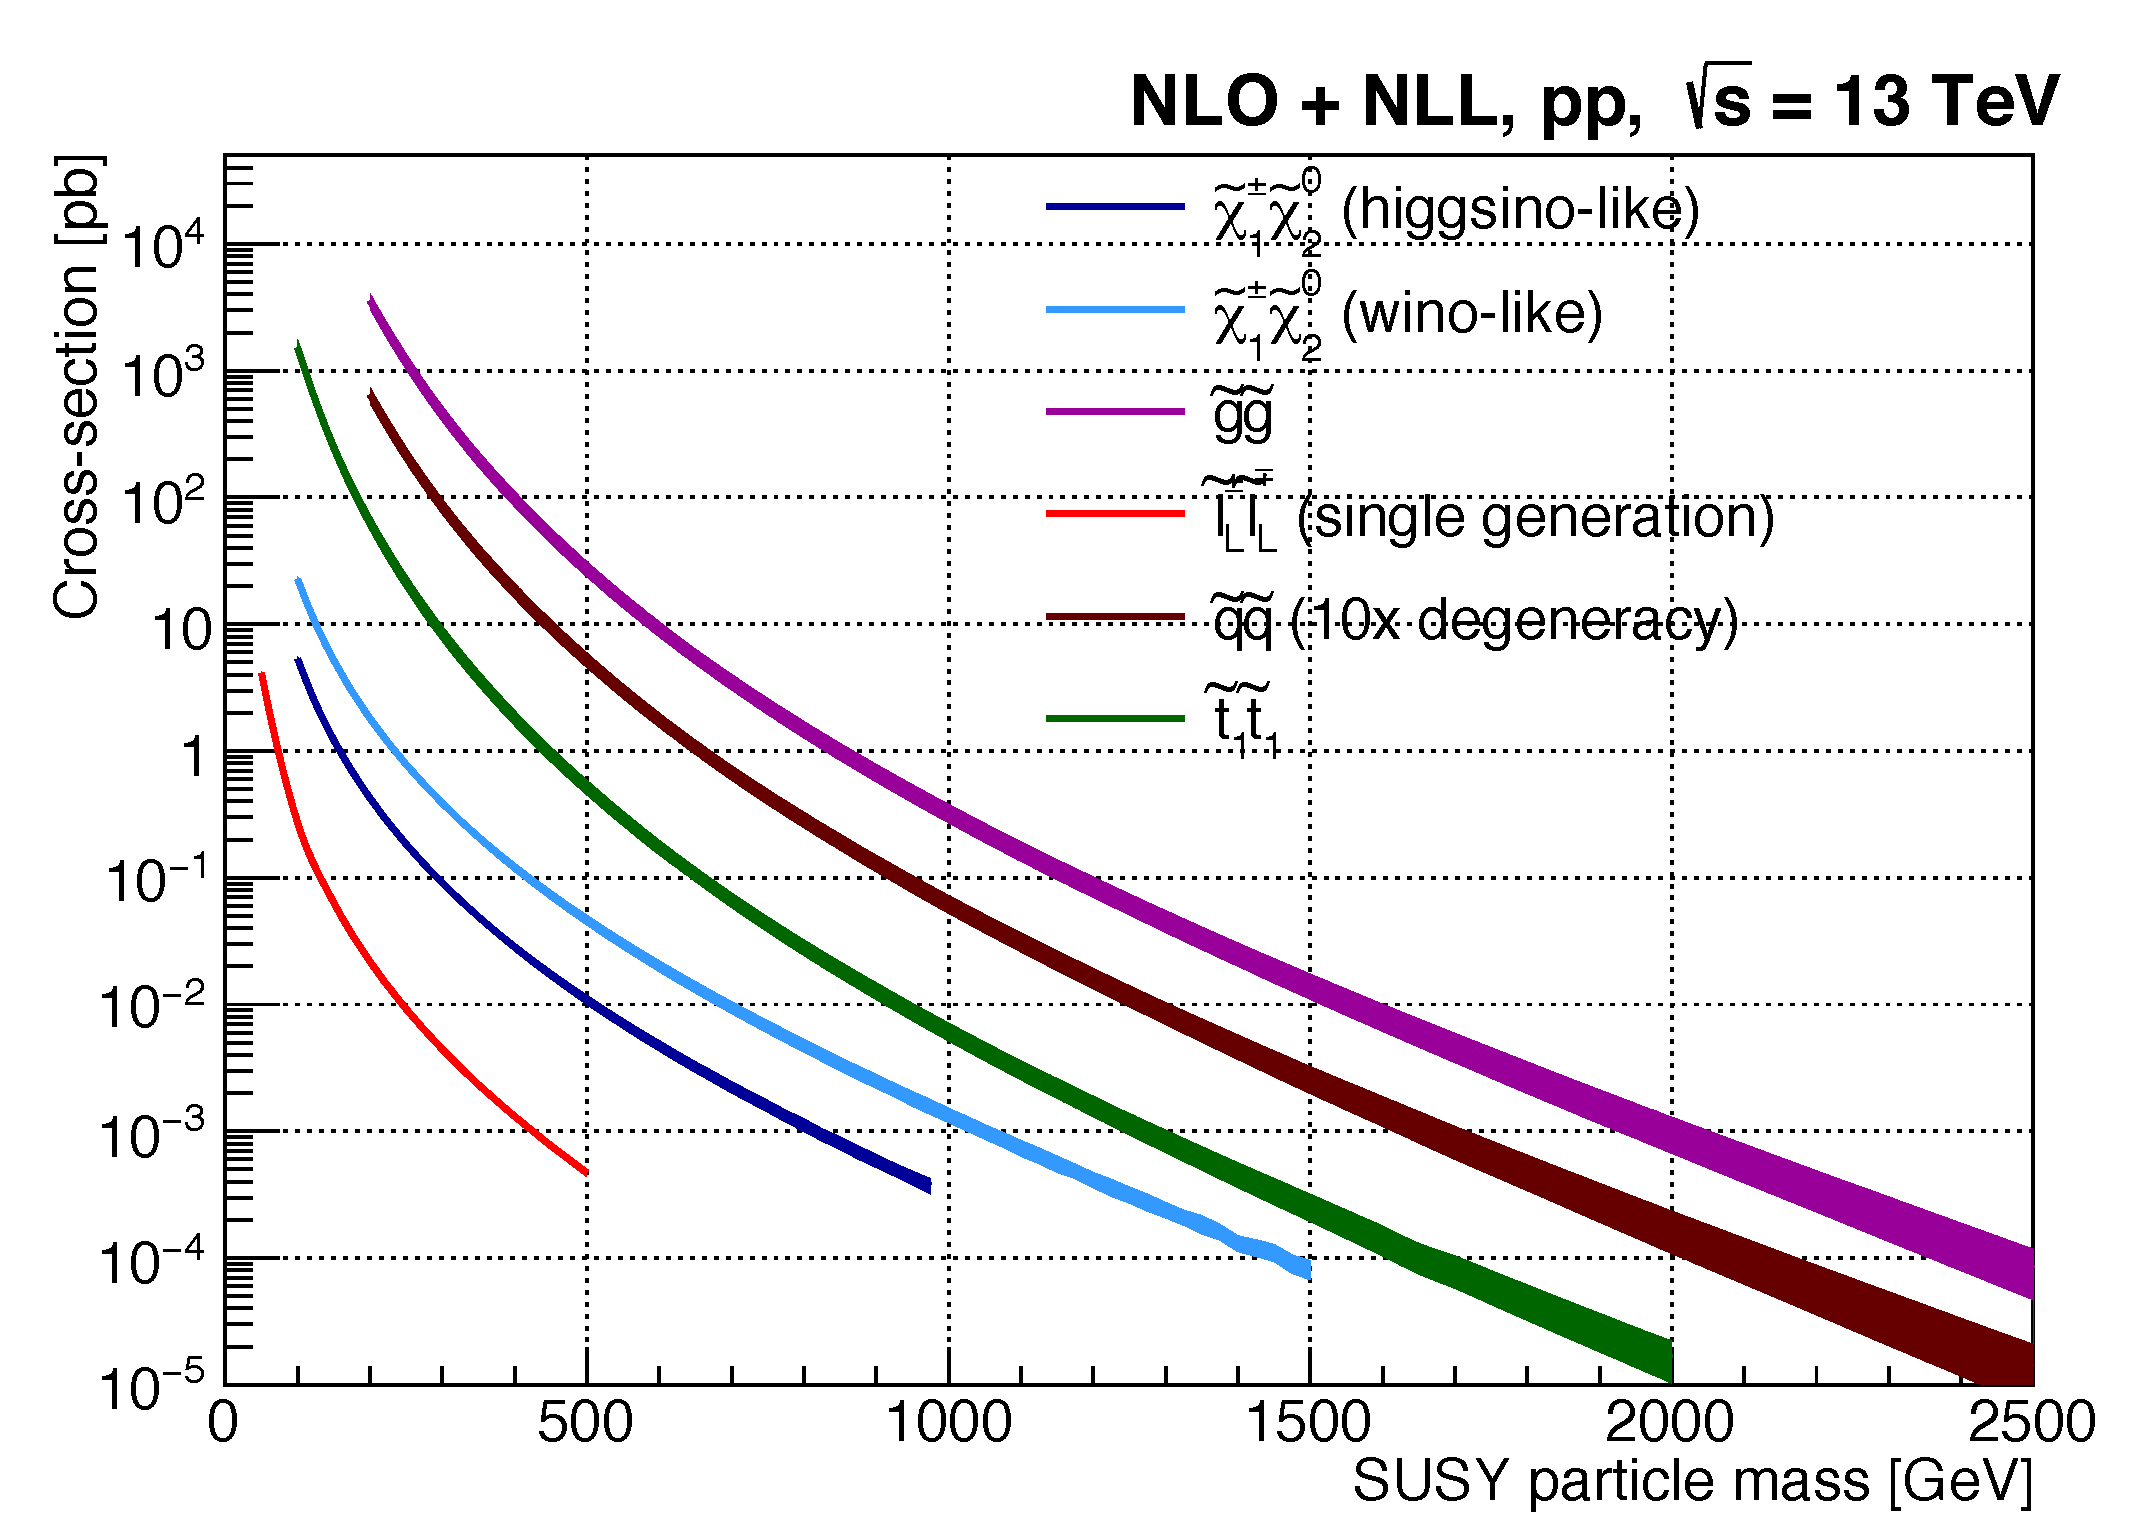
\includegraphics[width=0.65\textwidth]{figures/search_stop2l/SUSY_xsec_13TeV_v1}
        \caption{
            Production cross-section for the SUSY sparticles indicated in the legend,
            as a function of their mass, computed as in Ref.~\cite{SUSYXsec1}.
            The bands indicate the uncertainty due to the theoretical prediction of the production
            process.
            The green band indicates the \stopone production cross-section, relevant to the analysis
            described in the current chapter.
            For comparison, the production cross-section for SM top-quark pair-production is $\approx 830$\,pb at 13\,\TeV.
        }
        \label{fig:susy_xsec}
    \end{center}
\end{figure}

\FloatBarrier
%%%%%%%%%%%%%%%%%%%%%%%%%%%%%%%%%%%%%%%%%%%%%%%%%%%%%%%%%%%%%%%%%%%%%%%%%%%
%%%%%%%%%%%%%%%%%%%%%%%%%%%%%%%%%%%%%%%%%%%%%%%%%%%%%%%%%%%%%%%%%%%%%%%%%%%
%%%%%%%%%%%%%%%%%%%%%%%%%%%%%%%%%%%%%%%%%%%%%%%%%%%%%%%%%%%%%%%%%%%%%%%%%%%
%
% SIGNAL DESCRIPTION
%
%%%%%%%%%%%%%%%%%%%%%%%%%%%%%%%%%%%%%%%%%%%%%%%%%%%%%%%%%%%%%%%%%%%%%%%%%%%
%%%%%%%%%%%%%%%%%%%%%%%%%%%%%%%%%%%%%%%%%%%%%%%%%%%%%%%%%%%%%%%%%%%%%%%%%%%
%%%%%%%%%%%%%%%%%%%%%%%%%%%%%%%%%%%%%%%%%%%%%%%%%%%%%%%%%%%%%%%%%%%%%%%%%%%
\section{Description and Phenomenology of the Signal}
\label{sec:stop_pheno}


\subsection{Aside: SUSY Signal Grids}
\label{sec:susy_signal_grid}

\begin{figure}[!htb]
    \begin{center}
        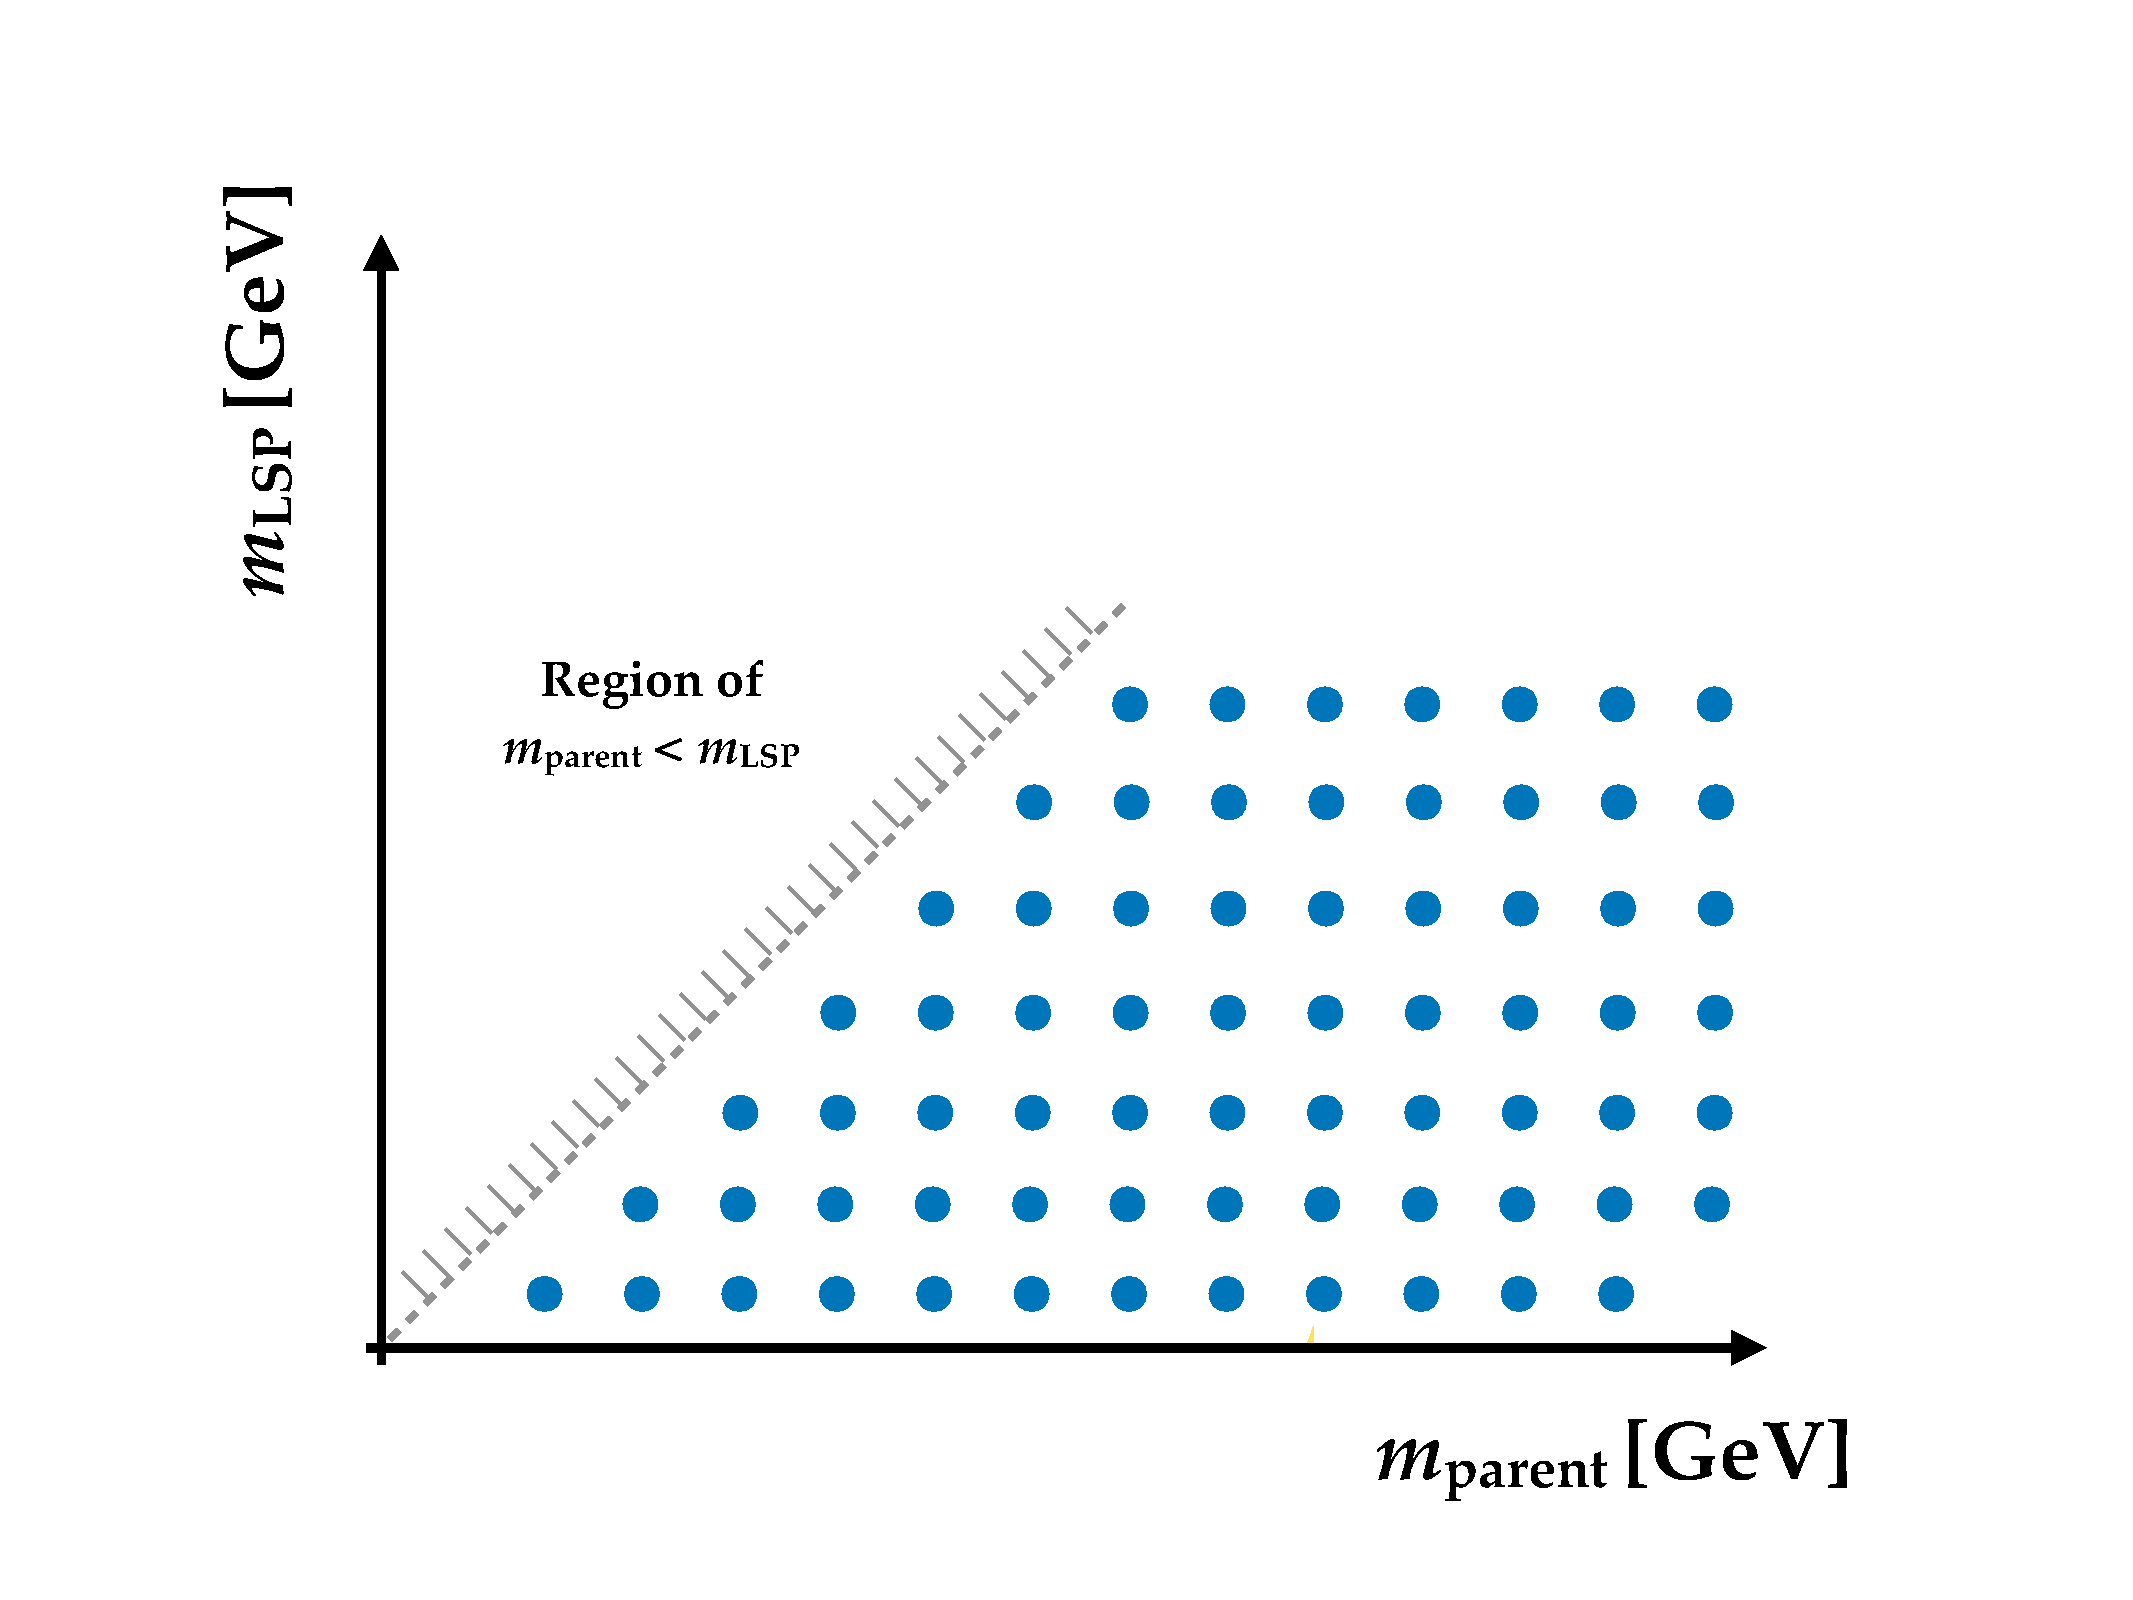
\includegraphics[width=0.6\textwidth]{figures/search_stop2l/signal/susy_signal_grid_example}
        \caption{
            Illustration of a SUSY signal grid.
            The blue points indicate points in the simplified model parameter space for which
            an individual MC-simulated sample is produced and available for use in analyses
            searching for the given type of SUSY.
        }
        \label{fig:susy_signal_grid}
    \end{center}
\end{figure}

Before the search for the \stopone can begin, MC simulated samples representing this process
must be obtained.
Once a given simplified model of the MSSM is chosen, specific points in the
$(m_{\stopone}, m_{\ninoone})$-plane are chosen and for each a separate MC simulated
sample is produced.
Each point represents a different hypothesis of SUSY, characterised by the specific masses
of the \stopone and \ninoone sparticles.
In ATLAS, this process of choosing points in the SUSY parameter space to produce MC simulated samples
is one requiring high levels of deliberation and discussion.
This is due to the fact that the simulation of complicated physics processes requires large amounts
of ATLAS' CPU resources, of which any given analysis group only has so much allocated, and so, among other things,
judicious choices about the number of events to be simulated at each point in the $(m_{\stopone}, m_{\ninoone})$-plane
must be made, as well as careful consideration of previous analyses' exclusion coverage in the same parameter space.
For this reason, the resulting SUSY `signal grids' are \textit{sparse}, as illustrated in Figure~\ref{fig:susy_signal_grid}.
Depending on how sparse the produced signal grid is, how the points are grouped, or how large each MC-sample at each
point is (in terms of number of MC events simulated), the resulting analyses' conclusions
can result in unphysical or even discontinous exclusion regions, which is clearly the case in the Run 1 searches
for the three-body decay of the \stopone, seen in Figure~\ref{fig:run1_stop_summary}.
When interpreting the results of SUSY searches, then, it is important to keep these facts in mind
so as to not over-interpret the results' statements about any fine-grained details of SUSY parameter space to
which the analyses are generally not sensitive.
Each point in a SUSY signal grid allows, rather, an analysis to make general statements about
an \textit{extended}, but still local, region of parameter space under the assumed simplified model.


%\subsection{Simulation of the Three-body Decay of the Stop Quark}
%\label{sec:stop_sim}
%
%The MC simulation of the three-body decay of the \stopone, used in the analysis discussed in 
%this chapter, is performed using \textsc{MadGraph5\_AMC@NLO}, including diagrams with up to
%two additional partons.
%In the three-body region of phase space of the \stopone decays, proceeding via off-shell
%intermediate SM top-quarks, the preservation of the \stopone left-right polarisation information
%must be handled with care.\footnote{The
%\stopone is of course a scalar particle, so it not chiral.
%The \stopL and \stopR  states that make up the \stopone and \stoptwo mass eigenstates refer, instead, 
%to their corresponding SM superpartner counterparts.
%}
%For this reason, produced \stop sparticles provided by \textsc{MadGraph5\_AMC@NLO} are decayed
%via \textsc{MadSpin}, described in Section~\ref{sec:mc_gen_afterburner}, which properly
%propagates the polarisation information of the massive \stopone particle into the
%off-shell and intermediate SM top-quark to which it decays, such that the kinematics of the
%$W$-boson ($\ell \nu$ system) and $b$-quark are correct.
%\textsc{Pythia} is used for the showering and fragmentation.

\subsection{Description of the Three-body Decay Final State}
\label{sec:stop_final_state}

\begin{figure}[!htb]
    \begin{center}
        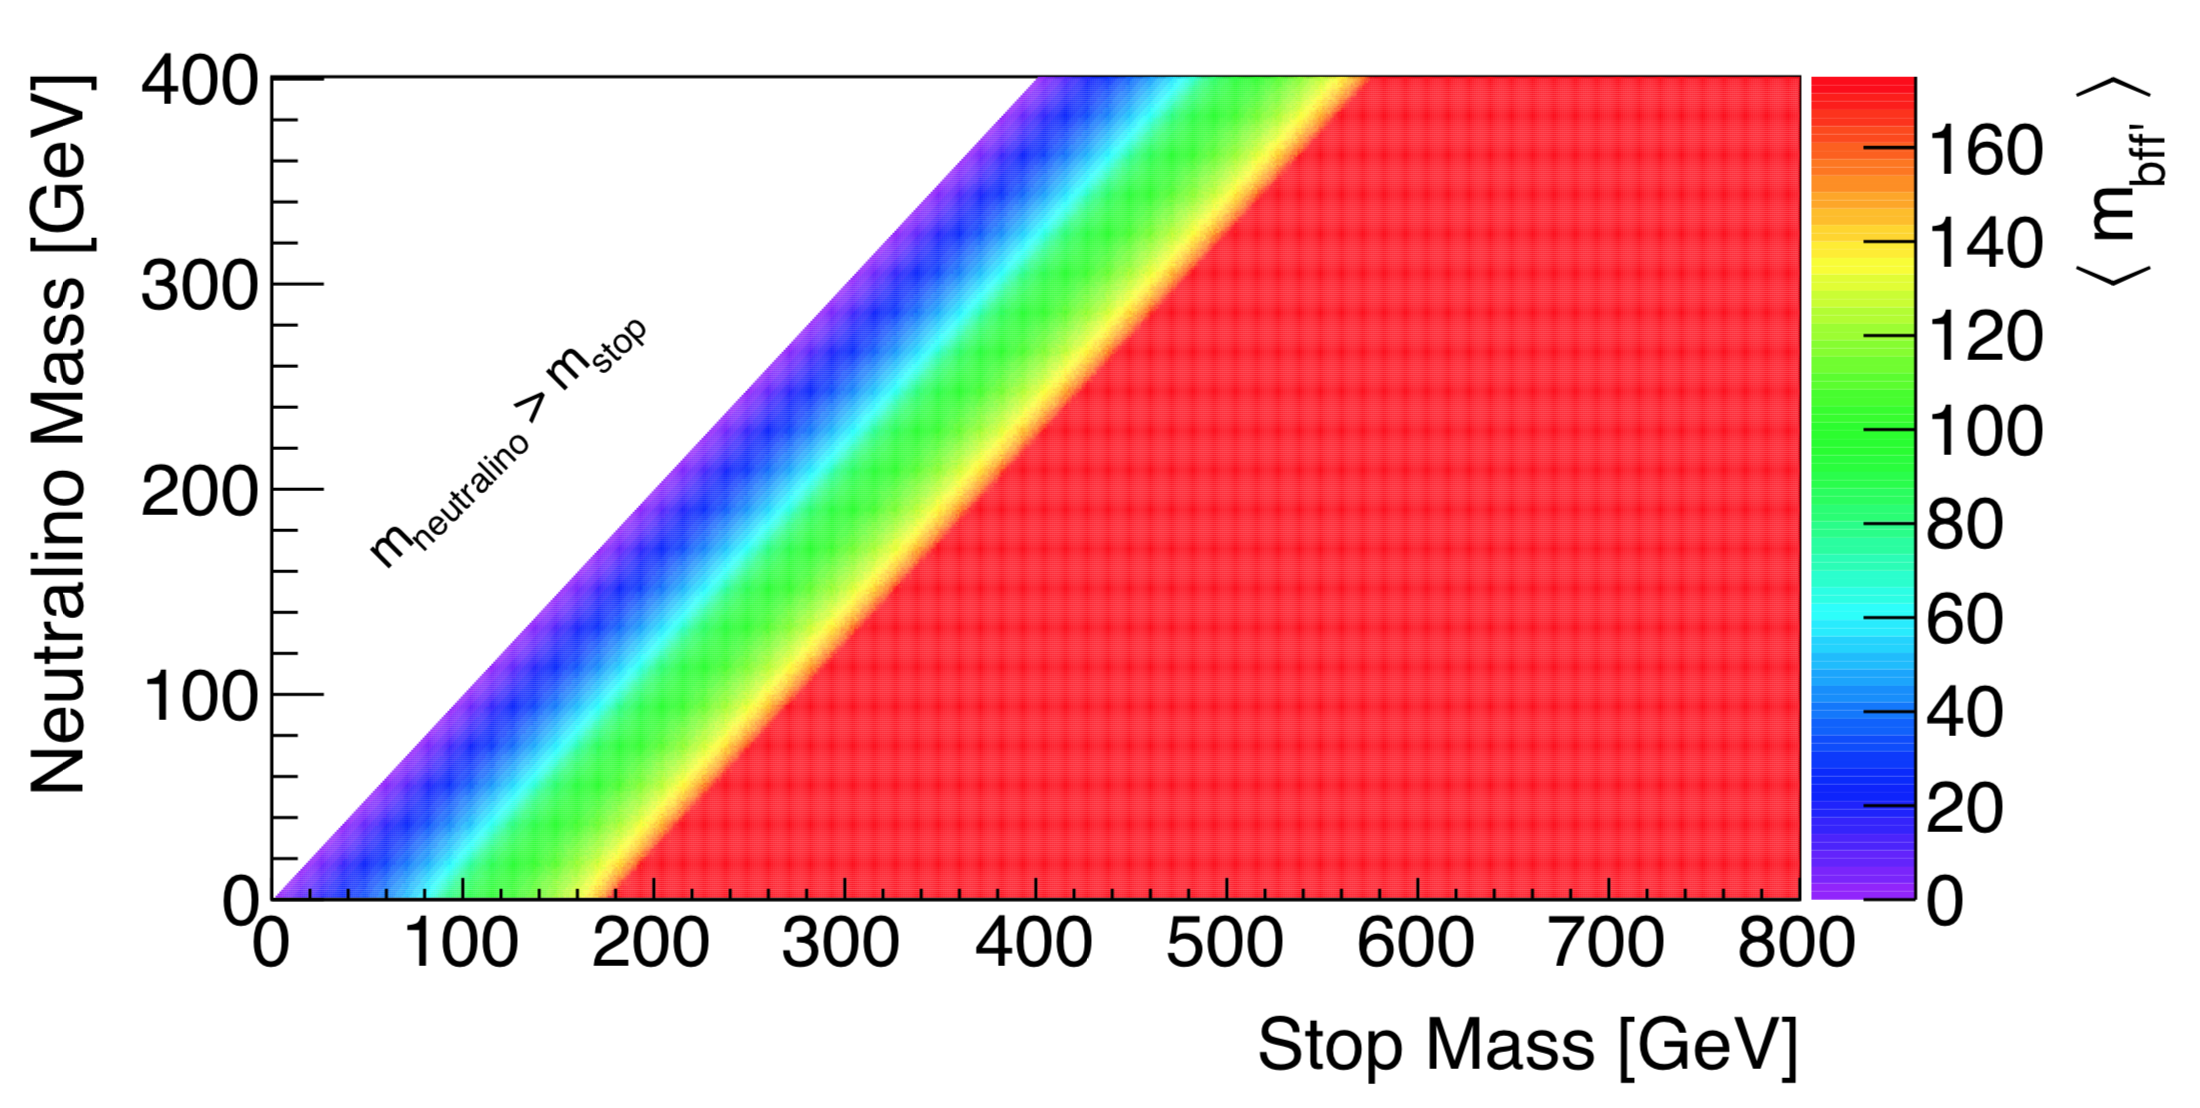
\includegraphics[width=0.75\textwidth]{figures/search_stop2l/nachman_stop_phase_space}
        \caption{
            Average invariant mass of the $b$-quark and SM fermions ($f f^{\prime}$) in the
            final state of the $\stopone \rightarrow b f f^{\prime} \ninoone$ decay, as a function of the mass
            of the \stopone and \ninoone particles.
            Figure taken from Ref.~\cite{Nachman:2016qyc}.
        }
        \label{fig:stop_phase_space}
    \end{center}
\end{figure}

In the three-body decays, the \stopone is assumed to decay via an off-shell SM top quark.
This is a kinematically suppressed region of phase space, as illustrated in Figure~\ref{fig:stop_phase_space},
which shows the average invariant mass of the \stopone decay products across the
two-, three-, and four-body decay regions of the $(m_{\stopone}, m_{\ninoone})$-plane (c.f. Figure~\ref{fig:stop_boundaries}).
In Figure~\ref{fig:stop_phase_space} the onset of the restricted phase space is clearly
visible as one drops beneath the $\sdiff = m_{\text{top}}$ line, at which point the final
state particle kinematics change rapidly.

The restricted phase space of the three-body \stopone decays has a large
impact on the analyses searching for the \stopone.
The $b$-quark children of the \stopone decays have decreasing momenta as one
moves from the $\sdiff = m_{\text{top}}$ kinematic boundary to that of $\sdiff = m_{W}$.
As a result, the $b$-jets that arise as a result of the $b$-quark hadronization process
are difficult to identify efficiently given the minimum 20\,\GeV~\pT~thresholds typical
of the ATLAS jet reconstruction and flavor-tagging identification algorithms.
This is illustrated in Figure~\ref{fig:stop_nbjets}, showing the $b$-tagged jet multiplicities
for various \stopone decay scenarios and how they compare to the dominant SM backgrounds.
As $\sdiff \rightarrow m_W$, the flavor-tagging algorithms are unable to identify the $b$-jets,
and the final state is kinematically similar to that of SM $WW$ production.

\begin{figure}[!htb]
    \begin{center}
        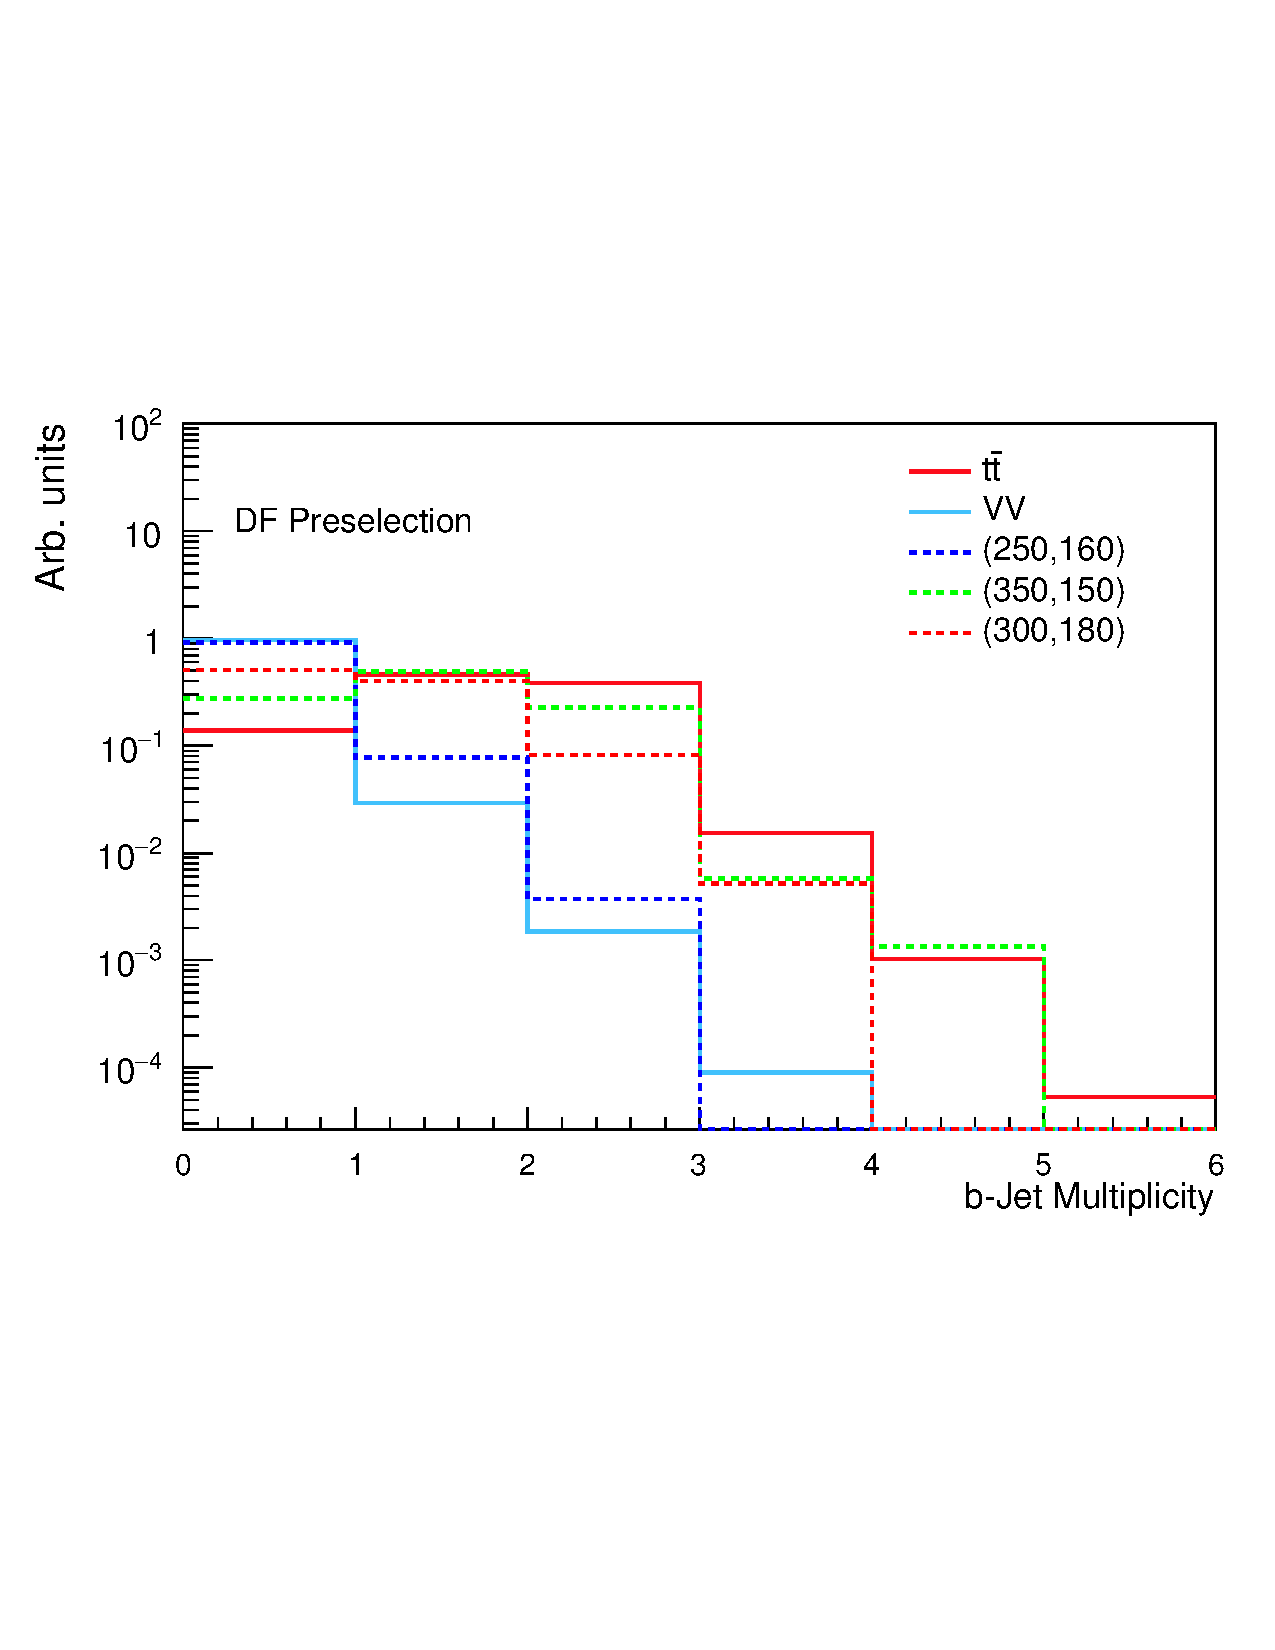
\includegraphics[width=0.7\textwidth]{figures/search_stop2l/strategy/comp_plots/dfpresel_nBJets}
        \caption{
            Normalised $b$-tagged jet multiplicity distributions for three \stopone signals (dashed lines),
            indicated by their position in the $(m_{\stopone}, m_{\ninoone})$-plane in the legend,
            and SM \ttbar~(solid red red) and diboson (VV) (solid blue line) production.
            It can be seen that the \stopone decays with $\sdiff \sim m_{\text{top}}$ have $b$-tagged jet
            multiplicities similar to that of SM \ttbar production.
            The \stopone decays with $\sdiff \rightarrow m_W$ tend to have zero reconstructed $b$-tagged jets.
            The selection, `DF Preselection', in the plot is that described in Table~\ref{tab:stop_preselection}.
        }
        \label{fig:stop_nbjets}
    \end{center}
\end{figure}

The \ninoone children of the \stopone decays, as with the $b$-quarks, also exhibit diminishing
momenta as one traverses the three-body region from the $\sdiff = m_{\text{top}}$ kinematic boundary to that of $\sdiff = m_W$.
As a result, the three-body \stopone decays do not have the typical signature of large
amounts of missing transverse momentum, typical of $R$-parity conserving SUSY decays.
The reduced impact of the \ninoone particles on the magnitude of the missing transverse momentum
furthers the three-body \stopone decays' resemblance to those of SM $WW$ production, in that
the primary carriers of missing transverse momentum are the neutrinos from the leptonic decays
of the $W$ bosons.

The three-body region allows for the on-shell production of the $W$ bosons.
For this reason, the leptons and neutrinos from their decay are not kinematically suppressed
in the same way as the $b$-quarks and \ninoone.
Their kinematics are therefore typical, in scale, to those of SM \ttbar~and $WW$ production.

\section{Event Selection and Object Definitions}
\label{sec:stop_event_sel}

In this section, the definitions of the event sample and of the reconstructed
objects used in the analysis are given.

%%%%%%%%%%%%%%%%%%%%%%%%%%%%%%%%%%%%%%%%%%%%%%%%%%%%%%%%%%%%%%%%%%%%%%%%%%%%%
%%%%%%%%%%%%%%%%%%%%%%%%%%%%%%%%%%%%%%%%%%%%%%%%%%%%%%%%%%%%%%%%%%%%%%%%%%%%%
%%%%%%%%%%%%%%%%%%%%%%%%%%%%%%%%%%%%%%%%%%%%%%%%%%%%%%%%%%%%%%%%%%%%%%%%%%%%%
%
% TRIGGER
%
%%%%%%%%%%%%%%%%%%%%%%%%%%%%%%%%%%%%%%%%%%%%%%%%%%%%%%%%%%%%%%%%%%%%%%%%%%%%%
%%%%%%%%%%%%%%%%%%%%%%%%%%%%%%%%%%%%%%%%%%%%%%%%%%%%%%%%%%%%%%%%%%%%%%%%%%%%%
%%%%%%%%%%%%%%%%%%%%%%%%%%%%%%%%%%%%%%%%%%%%%%%%%%%%%%%%%%%%%%%%%%%%%%%%%%%%%

\subsection{Trigger Selection}
\label{sec:stop_trigger}

As described in Section~\ref{sec:stop_final_state}, the $W$-bosons in the three-body
\stopone decays are on-shell and therefore lead to leptons whose kinematics are not
kinematically suppressed.
Each of the leptons is expected to have similar kinematics, given the relatively uncorrelated nature
of their decay, with transverse momenta on average at the scale of $m_W / 2 \sim 40\,\GeV$.
For this reason, the analysis can rely entirely on triggers based on the leptons.
The set of triggers used in the search for $\bWN$ is composed entirely of dilepton triggers,
having online lepton \pT~thresholds of of $10-18$\,GeV.

%%%%%%%%%%%%%%%%%%%%%%%%%%%%%%%%%%%%%%%%%%%%%%%%%%%%%%%%%%%%%%%%%%%%%%%%%%%%%
%%%%%%%%%%%%%%%%%%%%%%%%%%%%%%%%%%%%%%%%%%%%%%%%%%%%%%%%%%%%%%%%%%%%%%%%%%%%%
%%%%%%%%%%%%%%%%%%%%%%%%%%%%%%%%%%%%%%%%%%%%%%%%%%%%%%%%%%%%%%%%%%%%%%%%%%%%%
%
% OBJECT DEFINITIONS
%
%%%%%%%%%%%%%%%%%%%%%%%%%%%%%%%%%%%%%%%%%%%%%%%%%%%%%%%%%%%%%%%%%%%%%%%%%%%%%
%%%%%%%%%%%%%%%%%%%%%%%%%%%%%%%%%%%%%%%%%%%%%%%%%%%%%%%%%%%%%%%%%%%%%%%%%%%%%
%%%%%%%%%%%%%%%%%%%%%%%%%%%%%%%%%%%%%%%%%%%%%%%%%%%%%%%%%%%%%%%%%%%%%%%%%%%%%

\subsection{Object Definitions}
\label{sec:stop_object_def}

Here we describe the definitions of the leptons and jets used in the search for the
production of \stopone quarks.
The lepton (electron and muon) definitions are given in Table~\ref{tab:stop_lepton_def}
and the jet definitions are given in Table~\ref{tab:stop_jet_def}.
Discussion of the working points for lepton identification and isolation is given in
Section~\ref{sec:leptons}.
That of jets is found in Section~\ref{sec:jets} and \ref{sec:flavor_tagging}, for
jets, generically, and $b$-tagged jets, respectively.

The \pT~requirements of the leptons are such that they be on the plateau of the trigger
efficiency, as described in Section~\ref{sec:gather_data}.
The lepton isolation requirements are rather loose, given that a large contamination of 
fake and non-prompt leptons is not expected as a result of the requirement of two relatively
high-\pT~leptons.
The requirements on the impact parameter quantities $|d_0 / \sigma_{d_0}|$ and $|z_0 \times \sin \theta|$
further ensure that the leptons are likely to be prompt and have originated
from the primary hard-scatter vertex.

\begin{table}[!htb]
    \begin{center}
    \caption{
        Lepton definitions for the 2015+2016 analysis searching for the \stopone quark.
    }
    \label{tab:stop_lepton_def}
        \begin{tabular}{l | c | c | c | c }
        \hline
        \hline
            & \multicolumn{4}{c}{\textbf{Leptons}} \\
        \cline{2-5}
            & \multicolumn{2}{c}{\textbf{Electrons}} & \multicolumn{2}{c}{\textbf{Muons}} \\
        \cline{2-5}
            & \textbf{Baseline} & \textbf{Signal} & \textbf{Baseline} & \textbf{Signal} \\
        \hline
        \pT~requirement [GeV] & $(>10,>10)$ & $(>25,>20)$ & $(>10,>10)$ & $(>25,>20)$ \\
        $|\eta|$ requirement & \multicolumn{2}{c}{$<2.47$} & \multicolumn{2}{c}{$<2.4$} \\
        Identification WP & \texttt{Loose} & \texttt{Medium} & \multicolumn{2}{c}{\texttt{Medium}} \\
        Isolation & \multicolumn{4}{c}{\texttt{GradientLoose}} \\
        $|d_0 / \sigma_{d_0}|$ & $--$ & $<5$ & $--$ & $<3$ \\
        $|z_0 \times \sin \theta|$ [mm] & $--$ & $<0.5$ & $--$ & $<0.5$ \\
        \hline
        \hline
        \end{tabular}
    \end{center}
\end{table}

\begin{table}[!htb]
    \begin{center}
    \caption{
        Jet definitions for the 2015+2016 analysis searching for the \stopone quark.
    }
    \label{tab:stop_jet_def}
        \begin{tabular}{l | c | c}
            \hline
            \hline
                & \textbf{Jets} & \textbf{$b$-tagged Jets} \\
            \hline
            \pT~requirement [GeV] & \multicolumn{2}{c}{$>20$} \\
            $|\eta|$ requirement & $<2.8$ & $<2.4$ \\
            Pileup suppression & \multicolumn{2}{c}{ $\texttt{JVT} > 0.59$ if $\pT<60\,\GeV$~ and $|\eta| < 2.4$} \\
            Flavor-tagging WP & $--$ & $77\%$ \\
            \hline
            \hline
        \end{tabular}
    \end{center}
\end{table}

\subsection{Standard Event Pre-selection}
\label{sec:stop_preselection}

The starting sample of events, referred to as the analysis' \textit{preselection} level,
is defined simply and requires that events satisfy the following basic `data quality' (DQ) requirements:

\begin{itemize}
    \item No issues in any of the ATLAS subsystems were detected when the event was recorded
    \item A primary vertex with at least 2 tracks must be present in the event
    \item No cosmic muons\footnote{A cosmic muon is a reconstructed muon that is not consistent with
        having originated from the primary vertex, and therefore likely to have originated from
        a cosmic ray air shower.
        If a reconstructed muon does not satisfy both $|z_0| < 1$\,mm and $|d_0|<0.2$\,mm, it is considered
        a cosmic muon.} can be in the event
    \item If a poorly reconstructed jet is found in the event, likely to have arisen from stochastic
        noise bursts or issues in the calorimeter system, the event is rejected
\end{itemize}

Additionally, all events entering the analysis must also have two baseline level leptons (c.f. Table~\ref{tab:stop_lepton_def})
which have opposite electric charges, and must have a dilepton invariant mass $m_{\ell \ell}~>~20$\,GeV.
This latter requirement on $m_{\ell\ell}$ removes backgrounds due to low-mass $Z$-boson resonances, such as the $J/\psi$ ($m \sim 5\,\GeV$)
and $\Upsilon$ ($m \sim 11\,\GeV$) mesons. The complete preselection is summarized in Table~\ref{tab:stop_preselection}.

\begin{table}[!htb]
    \begin{center}
        \caption{
            Preselection summary for the 2015+2016 analysis searching for the \stopone quark.
            Signal level object requirements (Table~\ref{tab:stop_lepton_def} and \ref{tab:stop_jet_def}), as well as trigger requirements,
            are applied to the sample of events satisfying these requirements.
        }
        \label{tab:stop_preselection}
        \begin{tabular}{l|c| c}
            \hline
            \hline
            \textbf{Selection} & \textbf{SF Preselection} & \textbf{DF Preselection} \\
            \hline
            Lepton multiplicity & \multicolumn{2}{c}{$==2$ signal leptons} \\
            Dilepton flavor & $ee$ or $\mu \mu$ & $e\mu$ or $\mu e$ \\
            DQ requirements & \multicolumn{2}{c}{satisfied} \\
            Dilepton charge requirement & \multicolumn{2}{c}{opposite charge (OS)} \\
            Dilepton invariant mass, $m_{\ell\ell}$ [GeV] & \multicolumn{2}{c}{$>20$} \\
            \hline
            \hline
        \end{tabular}
    \end{center}
\end{table}

\section{Neural Network Based Signal Selection}
\label{sec:hh_strategy}

%%%%%%%%%%%%%%%%%%%%%%%%%%%%%%%%%%%%%%%%%%%%%%%%%%%%%%%%%%%%%%%%%%%%%%%%%%%%%%%%%%%
%%%%%%%%%%%%%%%%%%%%%%%%%%%%%%%%%%%%%%%%%%%%%%%%%%%%%%%%%%%%%%%%%%%%%%%%%%%%%%%%%%%
%%%%%%%%%%%%%%%%%%%%%%%%%%%%%%%%%%%%%%%%%%%%%%%%%%%%%%%%%%%%%%%%%%%%%%%%%%%%%%%%%%%
%
% NN 
%
%%%%%%%%%%%%%%%%%%%%%%%%%%%%%%%%%%%%%%%%%%%%%%%%%%%%%%%%%%%%%%%%%%%%%%%%%%%%%%%%%%%
%%%%%%%%%%%%%%%%%%%%%%%%%%%%%%%%%%%%%%%%%%%%%%%%%%%%%%%%%%%%%%%%%%%%%%%%%%%%%%%%%%%
%%%%%%%%%%%%%%%%%%%%%%%%%%%%%%%%%%%%%%%%%%%%%%%%%%%%%%%%%%%%%%%%%%%%%%%%%%%%%%%%%%%


The current analysis makes use of a multi-output classifier, one that does not simply classify
a single process against a single background label, but rather a classifier that provides multiple
output labels with each pertaining to a distinct class or process.
One of the easiest ways to build such a classifier is to take a multi-variate approach that
is by default suitable for multi-output classification: neural networks.

\subsection{Classifier Architecture}
\label{sec:nn_arch}

The analysis makes use of a deep-learning, neural network based approach.
The classifiers that we build are trained to classify $pp$ collision events according to
four potential class labels, inspired by the dominant expected background processes:
\begin{enumerate}
    \item Dilepton non-resonant $hh \rightarrow \bbww$
    \item SM top-quark processes ($\ttbar + Wt$), `Top'
    \item SM $Z$+jets processes, $Z \rightarrow \{ee,\mu\mu\}$
    \item SM $Z$+jets processes, $Z \rightarrow \tau\tau$
\end{enumerate}
The classifier is trained with separate labels for the $Z \rightarrow \{ee,\mu\mu\}$ and
$Z \rightarrow \tau\tau$ processes as these lead to clearly different final state kinematics.
The dilepton final state that we eventually select in the analysis is composed only of electrons and/or muons.
The $Z \rightarrow \tau\tau$ process contributes only in the cases where both $\tau$ leptons decay
leptonically.
The electrons and muons from these $\tau$ decays have very different kinematic signatures as compared
to those from the direct decays of the $Z$-bosons.
Allowing the classifier to learn how to distinguish between these $Z$ decays improves its overall performance
to separate the $hh$ signal process from the backgrounds.

We construct the neural network architecture using the \textsc{Keras}~\cite{chollet2015keras}
library, using \textsc{Tensorflow}~\cite{tensorflow2015} as a backend.
An illustration of the neural network architecture is given in Figure~\ref{fig:nn_arch}.
The network inputs are passed through a dense (fully-connected) layer,  which
is trained with a dropout layer, and then a second dense layer.
The final activation is a softmax activation~\cite{GoodFellowBook}.

\begin{figure}[!htb]
    \begin{center}
        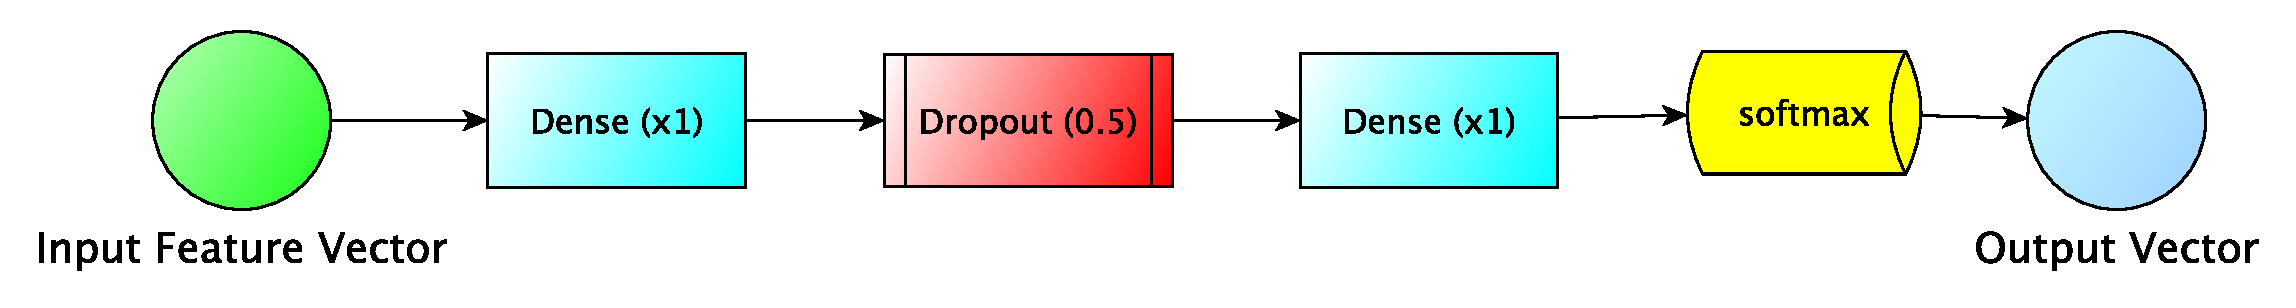
\includegraphics[width=0.85\textwidth]{figures/search_hh/mva/nn_arch_graph_updated}
        \caption{
            Illustration of the neural network graph employed in the analysis.
            The input feature vector has a length of 35 and the output vector is length 4,
            one for each of the targeted processes.
        }
        \label{fig:nn_arch}
    \end{center}
\end{figure}
Each of the dense layers are 250 nodes wide and  have their weights randomly initialized by sampling
from a truncated normal distribution centered on zero with a width given by $\sqrt{1/N_{\text{inputs}}}$, where
$N_{\text{inputs}}$ is the number of input features (the length of the input vector).
The activation functions for each of the dense layers are rectified linear units (`ReLu')~\cite{ReLu}.

Using an output layer with a softmax activation function allows one to interpret the outputs as
each representing a probability\footnote{
The use of the term `probability' here is not entirely correct, as the outputs are not \textit{strictly} probabilities given the fact that the network
does not know about the full set of possible processes that will be presented to it when it is used outside
of the training stage and in the analysis.
This is clear from the fact that the sum appearing in the denominator of Equation~\ref{eq:softmax_activation}
is not over the full set of processes that will be provided as input to the network when it is used
in the analysis.
The sum is only over those processes that we have decided to train the classifier to provide labels for.
Additionally, the labelled
processes are presented in artificial proportions during the training process, described in Section~\ref{sec:nn_train},
which may further prevent the network output's from being viewed as proper probabilities.
}
for the output's associated class ($hh$, Top, $Z \rightarrow \{ee,\mu\mu\}$,
or $Z \rightarrow \tau\tau$) given the inputs and for this reason it is commonly used for multi-class
neural network classifiers.
The association of the softmax activation with a class probability can be seen by its definition,
\begin{align}
    a_j = \frac{ e^{z_j} } { \sum\limits_k e ^{z_k} },
    \label{eq:softmax_activation}
\end{align}
where $a_j$ is the activation of the $j^{th}$ output neuron, the $z_i$ are the inputs to the output layer,
and $k$ runs over all output neurons.
It can be seen that if one sums over all outputs of a layer whose activation is given by Equation~\ref{eq:softmax_activation}
that the sum is equal to one.
Thus, the outputs of the softmax layer can be seen as a probability distribution.
For this reason, in the discussion to follow, we refer to the outputs of our neural network as `$p_i$',
where $i$ has four possibilities for each of the four outputs: $i \in \{ hh, \text{Top}, Z\rightarrow ee/\mu\mu, Z\rightarrow \tau\tau \}$.

The use of dropout layers during the training process of is a form of statistical learning regularization that is reminiscent
of ensemble methods in the non-deep-learning arena, such as random forests~\cite{RandomForestsBreiman2001}.
They act to randomly disable a tunable fraction of inputs during various points in the training stage~\cite{JMLRDropout}.
This tunable fraction is referred to as the \textit{dropout rate}.
The use of dropout regularization prevents nodes within the network from co-adapting too much, thus reducing
the effects of overtraining.
This is illustrated in Figure~\ref{fig:dropout_illustration}.
During each batch of events forwarded to the network during the training phase, the dropout layer disables
portions of the network and thereby presents a modified network to the inputs.
Conceptually, then, using dropout during training is similar to training a set of very many, different \textit{weak}
neural networks.
During test time, at the time when the neural network is actually being used in the analysis,
the network's weights, which have been determined after training over the set of thinned networks,
are scaled down by the dropout rate.
This is illustrated in Figure~\ref{fig:dropout_weight_scaling}.

\begin{figure}[!htb]
    \begin{center}
        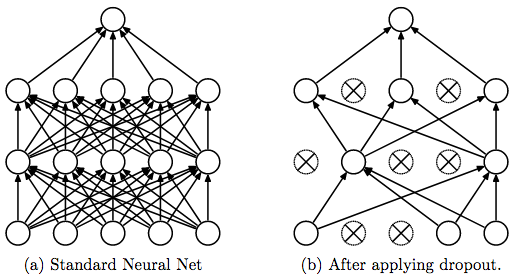
\includegraphics[width=0.7\textwidth]{figures/search_hh/mva/dropout_illustration}
        \caption{
            Illustration of dropout regularization. Figures taken from Ref.~\cite{JMLRDropout}.
            \textit{\textbf{Left}}: A standard neural network with two fully-connected layers.
            \textit{\textbf{Right}}: An example of a thinned network produced by applying dropout to the
                network on the left.
                The units with `X' have been dropped.
        }
        \label{fig:dropout_illustration}
    \end{center}
\end{figure}

\begin{figure}[!htb]
    \begin{center}
        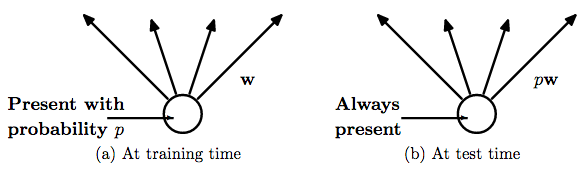
\includegraphics[width=0.7\textwidth]{figures/search_hh/mva/dropout_weight_scaling}
        \caption{
            Illustration of the dropout rate effect on the network weights. Figures taken from Ref.~\cite{JMLRDropout}.
            \textit{\textbf{Left}}: A node in a fully-connected layer at training time is present in the network with
                a probability equal to the dropout rate and is connected to the next layer with weights represented by $\bm{w}$.
            \textit{\textbf{Right}}: At test time, the node is present with 100\% probability but its weights are scaled down by the
                dropout rate, $p\bm{w}$.
        }
        \label{fig:dropout_weight_scaling}
    \end{center}
\end{figure}

\noindent
As mentioned above, the use of dropout regularization prevents nodes within the network from co-adapting
too much and forces the network to learn more robust features that are useful in conjunction with many 
different random subsets of the other nodes.
That is, dropout regularization ensures that the model is robust against the loss of any individual
``piece of evidence'' and is found to reduce the effects of overtraining, which improves the generalizability
of the trained classifier.

The neural network classifier used in the present analysis, illustrated in Figure~\ref{fig:nn_arch},
uses a single dropout layer acting on the first fully-connected node and is given a dropout rate of 50\%.

During training, the loss metric is the categorical crossentropy and the Adam optimization algorithm~\cite{AdamOptimizer} is used.\footnote{More
on categorical cross-entropy: \href{https://ml-cheatsheet.readthedocs.io/en/latest/loss_functions.html\#cross-entropy}
{https://ml-cheatsheet.readthedocs.io/en/latest/loss\_functions.html\#cross-entropy}}


%%%%%%%%%%%%%%%%%%%%%%%%%%%%%%%%%%%%%%%%%%%%%%%%%%%%%%%%%%%%%%%%%%%%%%%%%%%%%%%%%%%
%%%%%%%%%%%%%%%%%%%%%%%%%%%%%%%%%%%%%%%%%%%%%%%%%%%%%%%%%%%%%%%%%%%%%%%%%%%%%%%%%%%
%%%%%%%%%%%%%%%%%%%%%%%%%%%%%%%%%%%%%%%%%%%%%%%%%%%%%%%%%%%%%%%%%%%%%%%%%%%%%%%%%%%
%
% TRAINING AND ARCHITECTURE
%
%%%%%%%%%%%%%%%%%%%%%%%%%%%%%%%%%%%%%%%%%%%%%%%%%%%%%%%%%%%%%%%%%%%%%%%%%%%%%%%%%%%
%%%%%%%%%%%%%%%%%%%%%%%%%%%%%%%%%%%%%%%%%%%%%%%%%%%%%%%%%%%%%%%%%%%%%%%%%%%%%%%%%%%
%%%%%%%%%%%%%%%%%%%%%%%%%%%%%%%%%%%%%%%%%%%%%%%%%%%%%%%%%%%%%%%%%%%%%%%%%%%%%%%%%%%
\subsection{Definition of the Training Sample}
\label{sec:nn_train}

Prior to training a multi-variate classifier, such as the neural network described in Section~\ref{sec:nn_arch},
a well-defined set of simulated events for all labelled processed must be set aside for use in the training.
Ideally, these events are not to be used in the actual analysis, when the trained classifier is used only
for inference.
These two sets are referred to as the \textit{training set} and \textit{testing set}, respectively.

For defining our split between training and testing sets, the present analysis uses the `hold-out method' wherein
a fraction of the training events are set aside for use in evaluating classifier performance metrics
during the classifier training.
This is illustrated in Figure~\ref{fig:nn_sample_split}, where we use, out of our entire set of MC simulated
events, a percentage ($a\%$) for defining the training sample, with subsets of this set aside for evaluation
of the training performance.

\begin{figure}[!htb]
    \begin{center}
        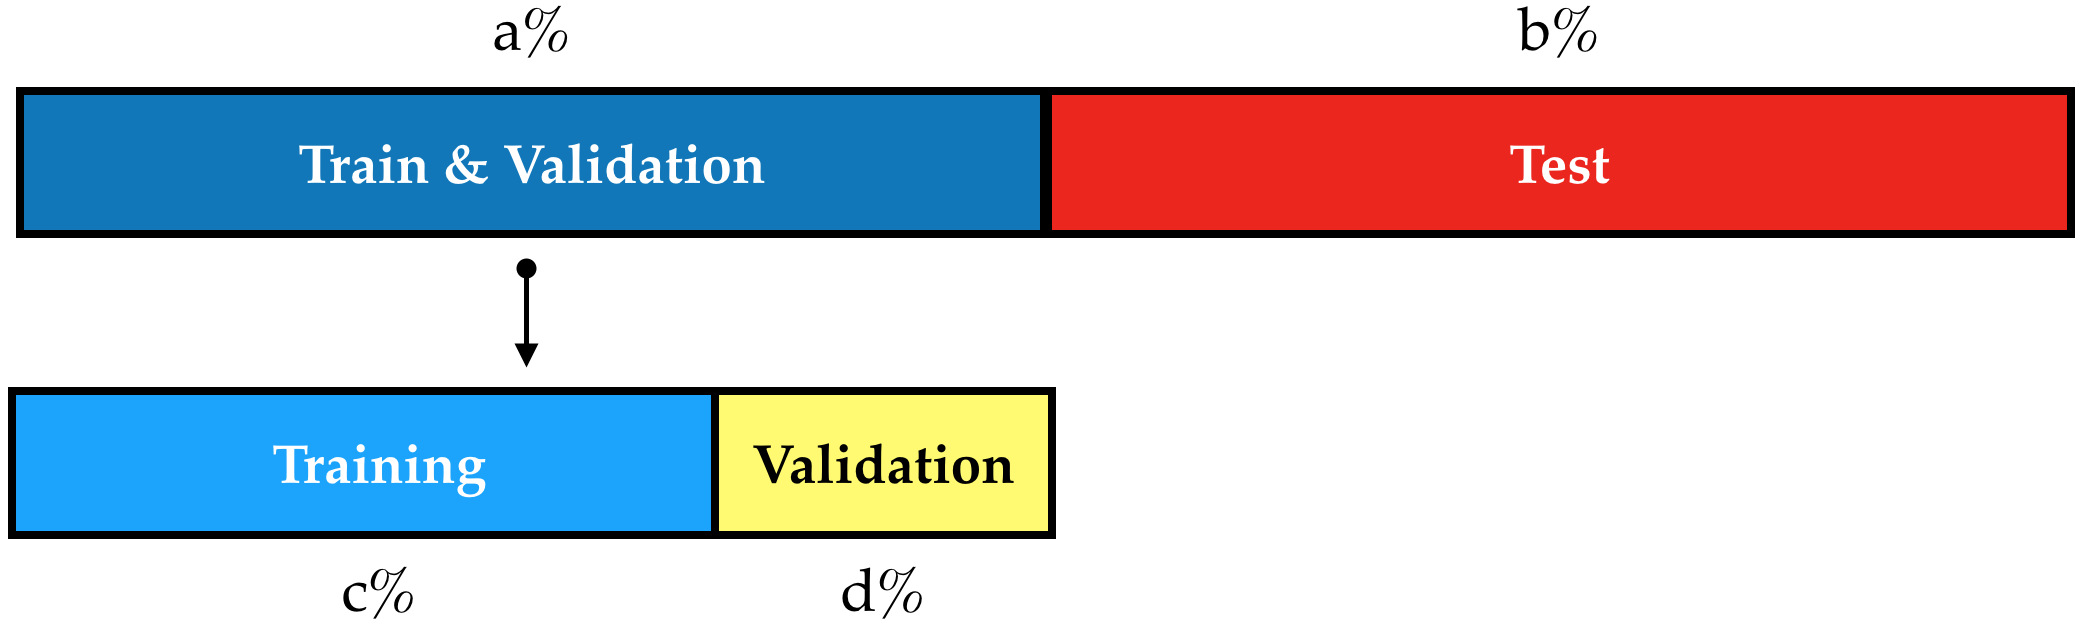
\includegraphics[width=0.7\textwidth]{figures/search_hh/mva/wwbb_nn_sample_breakdown}
        \caption{
            Illustration of the sample split used for training and testing the classifier.
            `Test' refers to the sample of events used at the analysis level (classifier inference only).
            `Training' and `Validation' events are used only during the training stage:
            Those events marked as `Training' are used for training of the classifier and those
            marked as `Validation' are used to evaluate the network performance metrics throughout
            the training process.
            $a$ is the percentage of the sample used for training and validation, $b$ the percentage used
            in the analysis, $c$ is the percentage of the Training data used for network training, and $d$ is the percentage
            of the Training data used for evaluating performance metrics.
            This gives $a\% + b\% = 100\%$ and $c\% + d\% = a\%$.
        }
        \label{fig:nn_sample_split}
    \end{center}
\end{figure}

During the training, the network is presented with inputs from MC-simulated events from each of the
four processed described above, each of which having a corresponding network output label.
The method used ensures an equal balance of processes in the training sample and revolves around
the total number of events existing in the MC sample of the signal process.
The number of events corresponding to $50\%$ of the total number of events in the signal MC sample
is set aside from each of the four samples to be used for training: $hh$, Top, $Z\rightarrow \{ee,\mu\mu\}$,
and $Z \rightarrow \tau\tau$.
The sum of all of these events corresponds to the `Training' sample in Figure~\ref{fig:nn_sample_split}.
As the neural network is trained, we want to make sure that at any given moment in the training process that the
network has a roughly equal chance of being presented with an event from any one of the four possible processes.
This ensures that no biases are learned by the network simply as a result of having an imbalanced training sample.
To avoid this, the training sample is randomly shuffled such that events in the Training sample are evenly distributed.
This breakdown and shuffling of the training events is illustrated in Figure~\ref{fig:nn_sample_shuffle}.
For the neural network trained in the present analysis, 20\% of the Training sample is set aside to make up
the Validation sample.

In addition to equally balancing the number of representative examples of each of the classes
that the neural network will be trained to identify, the MC events are not weighted during the training.
That is, the MC events are not weighted to their typical MC event weights associated with their
cross-section, reconstruction efficiencies, etc... nor are they given specific global class weights in the training.
All processes therefore have equal weight and equal sampling from the perspective of the training of the
classifier.
In the end, these parameters are additional \textit{hyperparameters} entering the training that must individually be tuned, if it is
desired to do so.
The choices made here, with respect to the process sampling and weighting, were made with the aim of designing the simplest training procedure possible.

All events used in the training procedure are required to satisfy the analysis' preselection
requirements defined in Section~\ref{sec:hh_event_selection} as well as having at least one $b$-tagged
jet, as detailed in Table~\ref{tab:train_selection}.
This is a rather loose selection --- looser than the one that will eventually be applied in the definition
of the analysis' SRs, CRs, and VRs --- but allows for larger numbers of events to be used in the training
process.

\begin{figure}[!htb]
    \begin{center}
        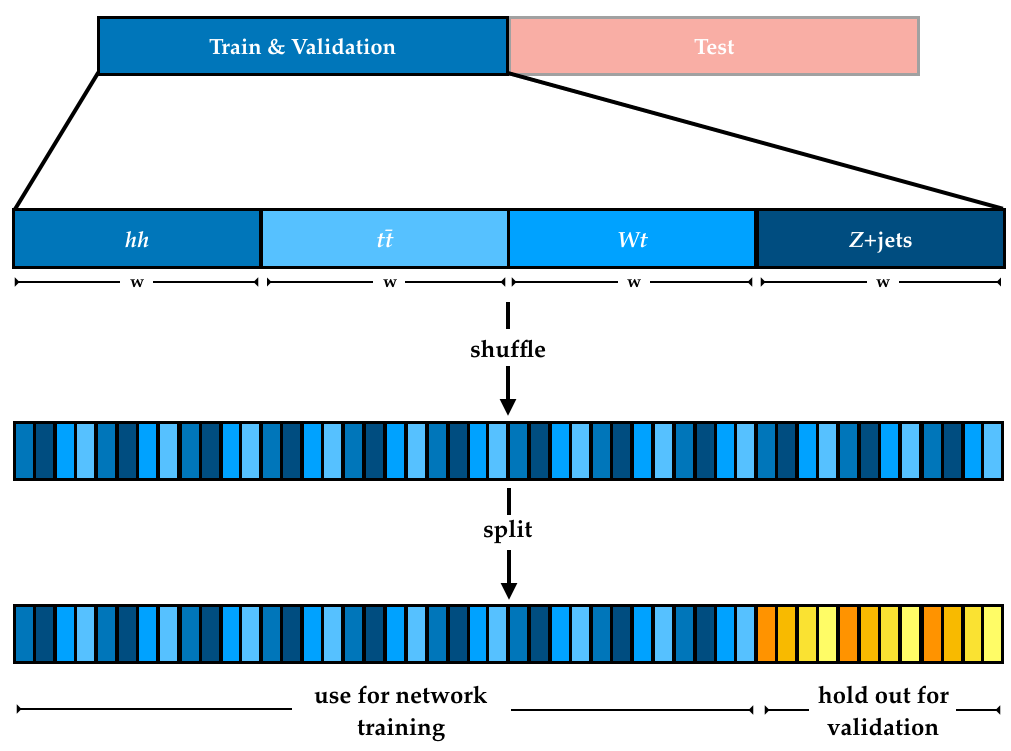
\includegraphics[width=0.8\textwidth]{figures/search_hh/mva/wwbb_nn_sample_split_detail}
        \caption{
            Detailed illustration of how the allocated training data is split into separate training
            and validation data samples.
            The sample size, or width $\bm{w}$, is defined by the signal MC sample: $\bm{w}$ is defined
            to be half of the events available in the signal MC.
            This width defines the sample sizes of the remaining three processes for which the neural network
            classifier provides an output label.
            Before the training process begins, these samples are randomly shuffled such that each process is distributed
            evenly throughout the entire set of events set aside for training.
            The validation sample is defined by holding out 20\% of the shuffled data.
            Labels and scales in the figure are illustrative only.
        }
        \label{fig:nn_sample_shuffle}
    \end{center}
\end{figure}

\begin{table}[!htb]
    \begin{center}
        \caption{
            Selection applied to events used in the neural network classifier training.
            In addition to this selection, the events must pass the standard preselection
            defined in Section~\ref{sec:hh_event_selection}.
        }
        \label{tab:train_selection}
        \begin{tabular}{l|c}
        \hline
        \hline
            \textbf{Observable} & \textbf{Selection} \\
            \hline
            Analysis preselection & Applied \\
            $b$-tagged jet multiplicity & $\ge 1$ \\
        \hline
        \hline
        \end{tabular}
    \end{center}
\end{table}

%%%%%%%%%%%%%%%%%%%%%%%%%%%%%%%%%%%%%%%%%%%%%%%%%%%%%%%%%%%%%%%%%%%%%%%%%%%%%%%%%%%
%%%%%%%%%%%%%%%%%%%%%%%%%%%%%%%%%%%%%%%%%%%%%%%%%%%%%%%%%%%%%%%%%%%%%%%%%%%%%%%%%%%
%%%%%%%%%%%%%%%%%%%%%%%%%%%%%%%%%%%%%%%%%%%%%%%%%%%%%%%%%%%%%%%%%%%%%%%%%%%%%%%%%%%
%
% PREPROCESSING
%
%%%%%%%%%%%%%%%%%%%%%%%%%%%%%%%%%%%%%%%%%%%%%%%%%%%%%%%%%%%%%%%%%%%%%%%%%%%%%%%%%%%
%%%%%%%%%%%%%%%%%%%%%%%%%%%%%%%%%%%%%%%%%%%%%%%%%%%%%%%%%%%%%%%%%%%%%%%%%%%%%%%%%%%
%%%%%%%%%%%%%%%%%%%%%%%%%%%%%%%%%%%%%%%%%%%%%%%%%%%%%%%%%%%%%%%%%%%%%%%%%%%%%%%%%%%

\subsection{Input Features and their Preprocessing}
\label{sec:nn_preprocessing}

The thirty five inputs to the neural network are detailed in Table~\ref{tab:nn_inputs}.
They are composed of low level features of the visible final state objects, such
as the lepton and jet momenta, as well as observables sensitive to the Higgs hemisphere
topology characterising the dilepton $hh \rightarrow \bbww$ signal and described in Section~\ref{sec:hh_pheno}.

As discussed in Section~\ref{sec:nn_train} and indicated in Table~\ref{tab:train_selection}, the neural network
classifier is trained on events with the minimal requirement that they pass the analysis preselection requirements
and that there be at least one $b$-tagged jet in the event.
One can see by comparing the training event selection in Table~\ref{tab:train_selection} and the network
inputs in Table~\ref{tab:nn_inputs}, that there will be cases where several of the input features
will be ill-defined.
Specifically, there will be cases wherein a training event has only a single $b$-tagged jet in which
case the observables listed in Table~\ref{tab:nn_inputs} that require at least two $b$-tagged jets
are not defined.
What is done in these cases is to fix the two $b$-tagged jet observables in Table~\ref{tab:nn_inputs}
for these one $b$-tagged jet events to the \textit{mean} of the corresponding observable as seen in
those events that have at least two $b$-tagged jets.
The mean for each observable is defined using as sample of events all those events that make
up the training sample, inclusive of all four of the trained-against processes.
That is, distributions of all observables are constructed for each of four processes ($hh$, Top, $Z \rightarrow \{ee,\mu\mu\}$, $Z \rightarrow \tau\tau$)
for those events with at least two $b$-tagged jets.
For each observable, the four process-specific distributions are summed together to produce the final
distribution from which the mean value is extracted.
During the network training, these mean values are used for the observables requiring
at least two $b$-tagged jets to be defined in those events only having a single $b$-tagged jet.
This procedure, illustrated in Figure~\ref{fig:nn_feature_means}, is done only during the training phase of the classifier.

A second stage of input feature pre-processing is applied to all features provided to the classifier,
done at both the training and in the testing stage of the analysis.
This stage is a standardization step and involves, for each event, the shifting of each input feature by its mean value and scaling
its value by its pre-shifted variance,
\begin{align*}
    x^{\prime} = \frac{x - \langle x \rangle}{\sigma_x}.
\end{align*}
This type of standardization is fairly standard practice, and is done so that all inputs provided
to the neural network are on a similar range --- centered at zero and with common spread --- thereby
making it easier for the classifier to learn the relationships (i.e. correlations) between the inputs,
as opposed to their absolute scales.
These standardization schemes additionally aid in numerically stabilizing the neural network's gradient-descent-based
optimization procedures employed during the training phase.
The standardization described above and used in the present analysis is illustrated in Figure~\ref{fig:nn_feature_standard}.


\begin{table}[!htb]
    \begin{center}
    \begin{footnotesize}
    \caption{
        Description of the variables used as inputs to the DNN classifier.
    }
    \label{tab:nn_inputs}
    \begin{tabularx}{\textwidth}{l |p{14.5cm}l}
    \toprule
    \hline
    ($p_{T}$, $\eta$, $\phi$) & $p_{T}$, $\eta$, and $\phi$ of the leptons, leading two signal jets, and leading two $b$-tagged jets \\
    Dilepton flavour & Whether the event is composed of two electrons, two muons, or one of each \\
    $\Delta R_{\ell\ell}$, $|\Delta \phi_{\ell\ell}|$   & $\Delta R$ and magnitude of the $\Delta \phi$ between the two leptons \\
    $m_{\ell\ell}$, $p_{T}^{\ell\ell}$  & Invariant mass and the transverse momentum of the dilepton system \\
    $\met$, $\met$-$\phi$ & Magnitude of the missing transverse momentum vector and its $\phi$ component \\
    $|\Delta \phi (\ptmiss, \ptvec{\ell}{\ell})|$ & Magnitude of the $\Delta \phi$ between the \ptmiss and the transverse momentum of the dilepton system \\
    $|\ptmiss + \ptvec{\ell}{\ell}|$ & Magnitude of the vector sum of the \ptmiss and the transverse momentum of the dilepton system \\
    Jet multiplicities & Numbers of $b$-tagged and non-$b$-tagged jets \\
    $|\Delta \phi_{bb}|$ & Magnitude of the $\Delta \phi$ between the leading two $b$-tagged jets \\ [0.08cm]
    $\mtbb$ & \mttwo using the leading two $b$-tagged jets as the visible inputs and \ptmiss as invisible input\\ [0.1cm]
    $\httwo$ & Numerator appearing in Equation~\ref{eq:ht2ratio_def}, \htnum \\
    $\htratio$ & As defined in Equation~\ref{eq:ht2ratio_def} \\
    \hline
    \bottomrule
    \end{tabularx}
    \end{footnotesize}
    \end{center}
\end{table}

\begin{figure}[!htb]
    \begin{center}
        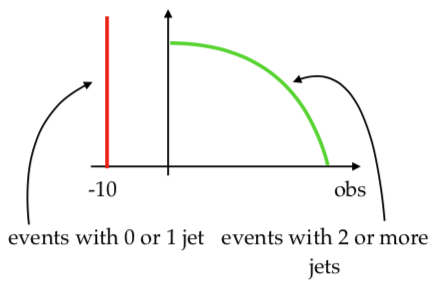
\includegraphics[width=0.45\textwidth]{figures/search_hh/mva/nn_feature_illdefined}
        \raisebox{0.5cm}{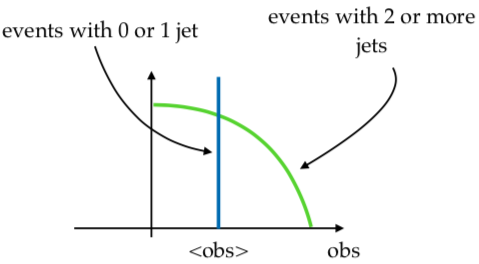
\includegraphics[width=0.54\textwidth]{figures/search_hh/mva/nn_feature_okdefined}}
        \caption{
            Illustration of setting events with ill-defined observables to the mean of those observables
            as measured in events in which the observables are properly defined.
            \textit{\textbf{Left}}: A counter-example in which ill-defined events' observables are set to a fixed default
                value outside of the physical range (a common practice).
                This would bias the mean of the properly defined events to the left.
            \textit{\textbf{Right}}: Setting the ill-defined events' observables to the mean of the observable
                as seen in events where the observable is properly defined.
                Doing this does not affect the overall mean of the observable in events where the
                observable is well-defined, nor does it lead to a discontinuity in the distributions of observables
                being provided to the classifier during its training.
        }
        \label{fig:nn_feature_means}
    \end{center}
\end{figure}

\begin{figure}[!htb]
    \begin{center}
        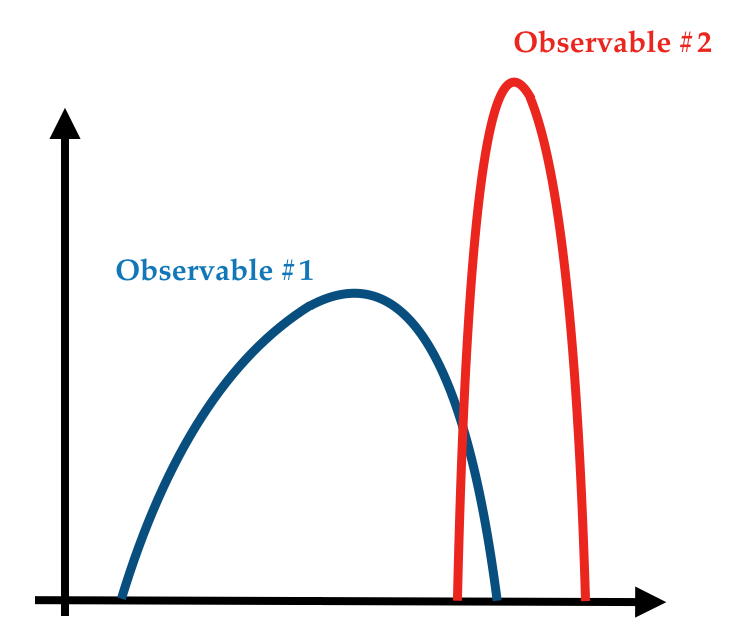
\includegraphics[width=0.38\textwidth]{figures/search_hh/mva/feature_standard_1}
        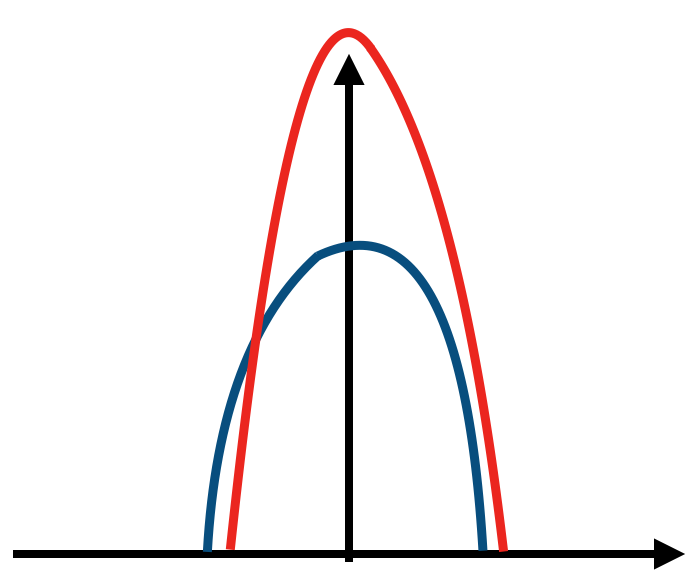
\includegraphics[width=0.38\textwidth]{figures/search_hh/mva/feature_standard_2}
        \caption{
            Illustration of the input feature standardization that occurs for all input features,
            for all events, prior to the features being fed into the neural network classifier
            (for both training and testing).
            \textit{\textbf{Left}}: Two different observables (overlaid for comparison) that have quite
            different shapes. Observable \#1 has a larger variance and is shifted to the left with
            respect to Observable \#2, which is a quite localized observable.
            \textit{\textbf{Right}}: After standardization, both observables have roughly the same
            mean (zero) and their widths have been scaled such that they are similar.
        }
        \label{fig:nn_feature_standard}
    \end{center}
\end{figure}

Note that it is this standardization procedure which motivates the method that
is used for augmenting the two $b$-tagged jet observables in the one $b$-tagged jet events.
By setting the ill-defined observables in the on $b$-tagged jet events to the mean of the observables
as defined in the two $b$-tagged jet events, we theoretically prevent the neural network from learning
from that specific observable on such events since after standardization they will be shifted towards zero
and any spurious correlation will be minimized.
In practice, however, it has been found that the specific choice of the scheme used for augmenting the two $b$-tagged jet observables
in one $b$-tagged jet events has little meaningful impact on the performance of the classifier.
The one described above has been used as it is the simplest, practically speaking.

The pre-processing steps, happening at each event and in order, are as follows:
\begin{enumerate}
    \item Augment two $b$-tagged jet observables for one $b$-tagged jet events (if applicable)
    \item Perform input feature standardization
    \item Feed inputs to network (either for training or for use in the analysis)
\end{enumerate}

%%%%%%%%%%%%%%%%%%%%%%%%%%%%%%%%%%%%%%%%%%%%%%%%%%%%%%%%%%%%%%%%%%%%%%%%%%%%%%%%%%%
%%%%%%%%%%%%%%%%%%%%%%%%%%%%%%%%%%%%%%%%%%%%%%%%%%%%%%%%%%%%%%%%%%%%%%%%%%%%%%%%%%%
%%%%%%%%%%%%%%%%%%%%%%%%%%%%%%%%%%%%%%%%%%%%%%%%%%%%%%%%%%%%%%%%%%%%%%%%%%%%%%%%%%%
%
% NN  TRAINING
%
%%%%%%%%%%%%%%%%%%%%%%%%%%%%%%%%%%%%%%%%%%%%%%%%%%%%%%%%%%%%%%%%%%%%%%%%%%%%%%%%%%%
%%%%%%%%%%%%%%%%%%%%%%%%%%%%%%%%%%%%%%%%%%%%%%%%%%%%%%%%%%%%%%%%%%%%%%%%%%%%%%%%%%%
%%%%%%%%%%%%%%%%%%%%%%%%%%%%%%%%%%%%%%%%%%%%%%%%%%%%%%%%%%%%%%%%%%%%%%%%%%%%%%%%%%%

\subsection{Training Procedure}
\label{sec:nn_train_procedure}

For illustration purposes, Figure~\ref{fig:nn_batches} illustrates the process of training
a neural network with many batches of events, the sum total of which comprise the entirety
of the events set aside for training.
An epoch refers to the point at which every single event in the training sample has been fed into
the network.
The neural network classifier described in Section~\ref{sec:nn_arch} is trained using the 
sample of events described in Section~\ref{sec:nn_train} using a batch size of 2,000 events,
with a maximum number of training epochs set to a large number ($\mathcal{O}(100)$).

Neural network classifiers typically train for many epochs, meaning that every event in the training
sample is used multiple times in the training procedure.
The training procedure used in the present analysis relies on an `early-stopping' metric that is imposed during the training phase such that, if the network's learning
begins to plateau, it will stop the training whether or not the maximum number of epochs has been
reached.
The metric used to determine whether the early-stopping criteria has been met is the neural network
loss value as evaluated on the held-out validation sample of events.
The aim of the network, during the training phase, is to minimize the loss.
Therefore, once the metric used for defining the early-stopping criteria hits a (minimum) plateau
it will stop after a configurable number of epochs in which no new minimum is found.
This configurable number, referred to as the `patience', is set to 20 for the classifier used in the present analysis.
%leading to a typical training phase lasting for 80 to 110 epochs.
Figure~\ref{fig:nn_epoch_overtrain} shows several training performance metrics evaluated on both the
training and held-out validation data, from which it can be seen that setting the patience parameter to 20
allows the network to maximize its learning before effects of overtraining begin to set in.

\begin{figure}[!htb]
    \begin{center}
        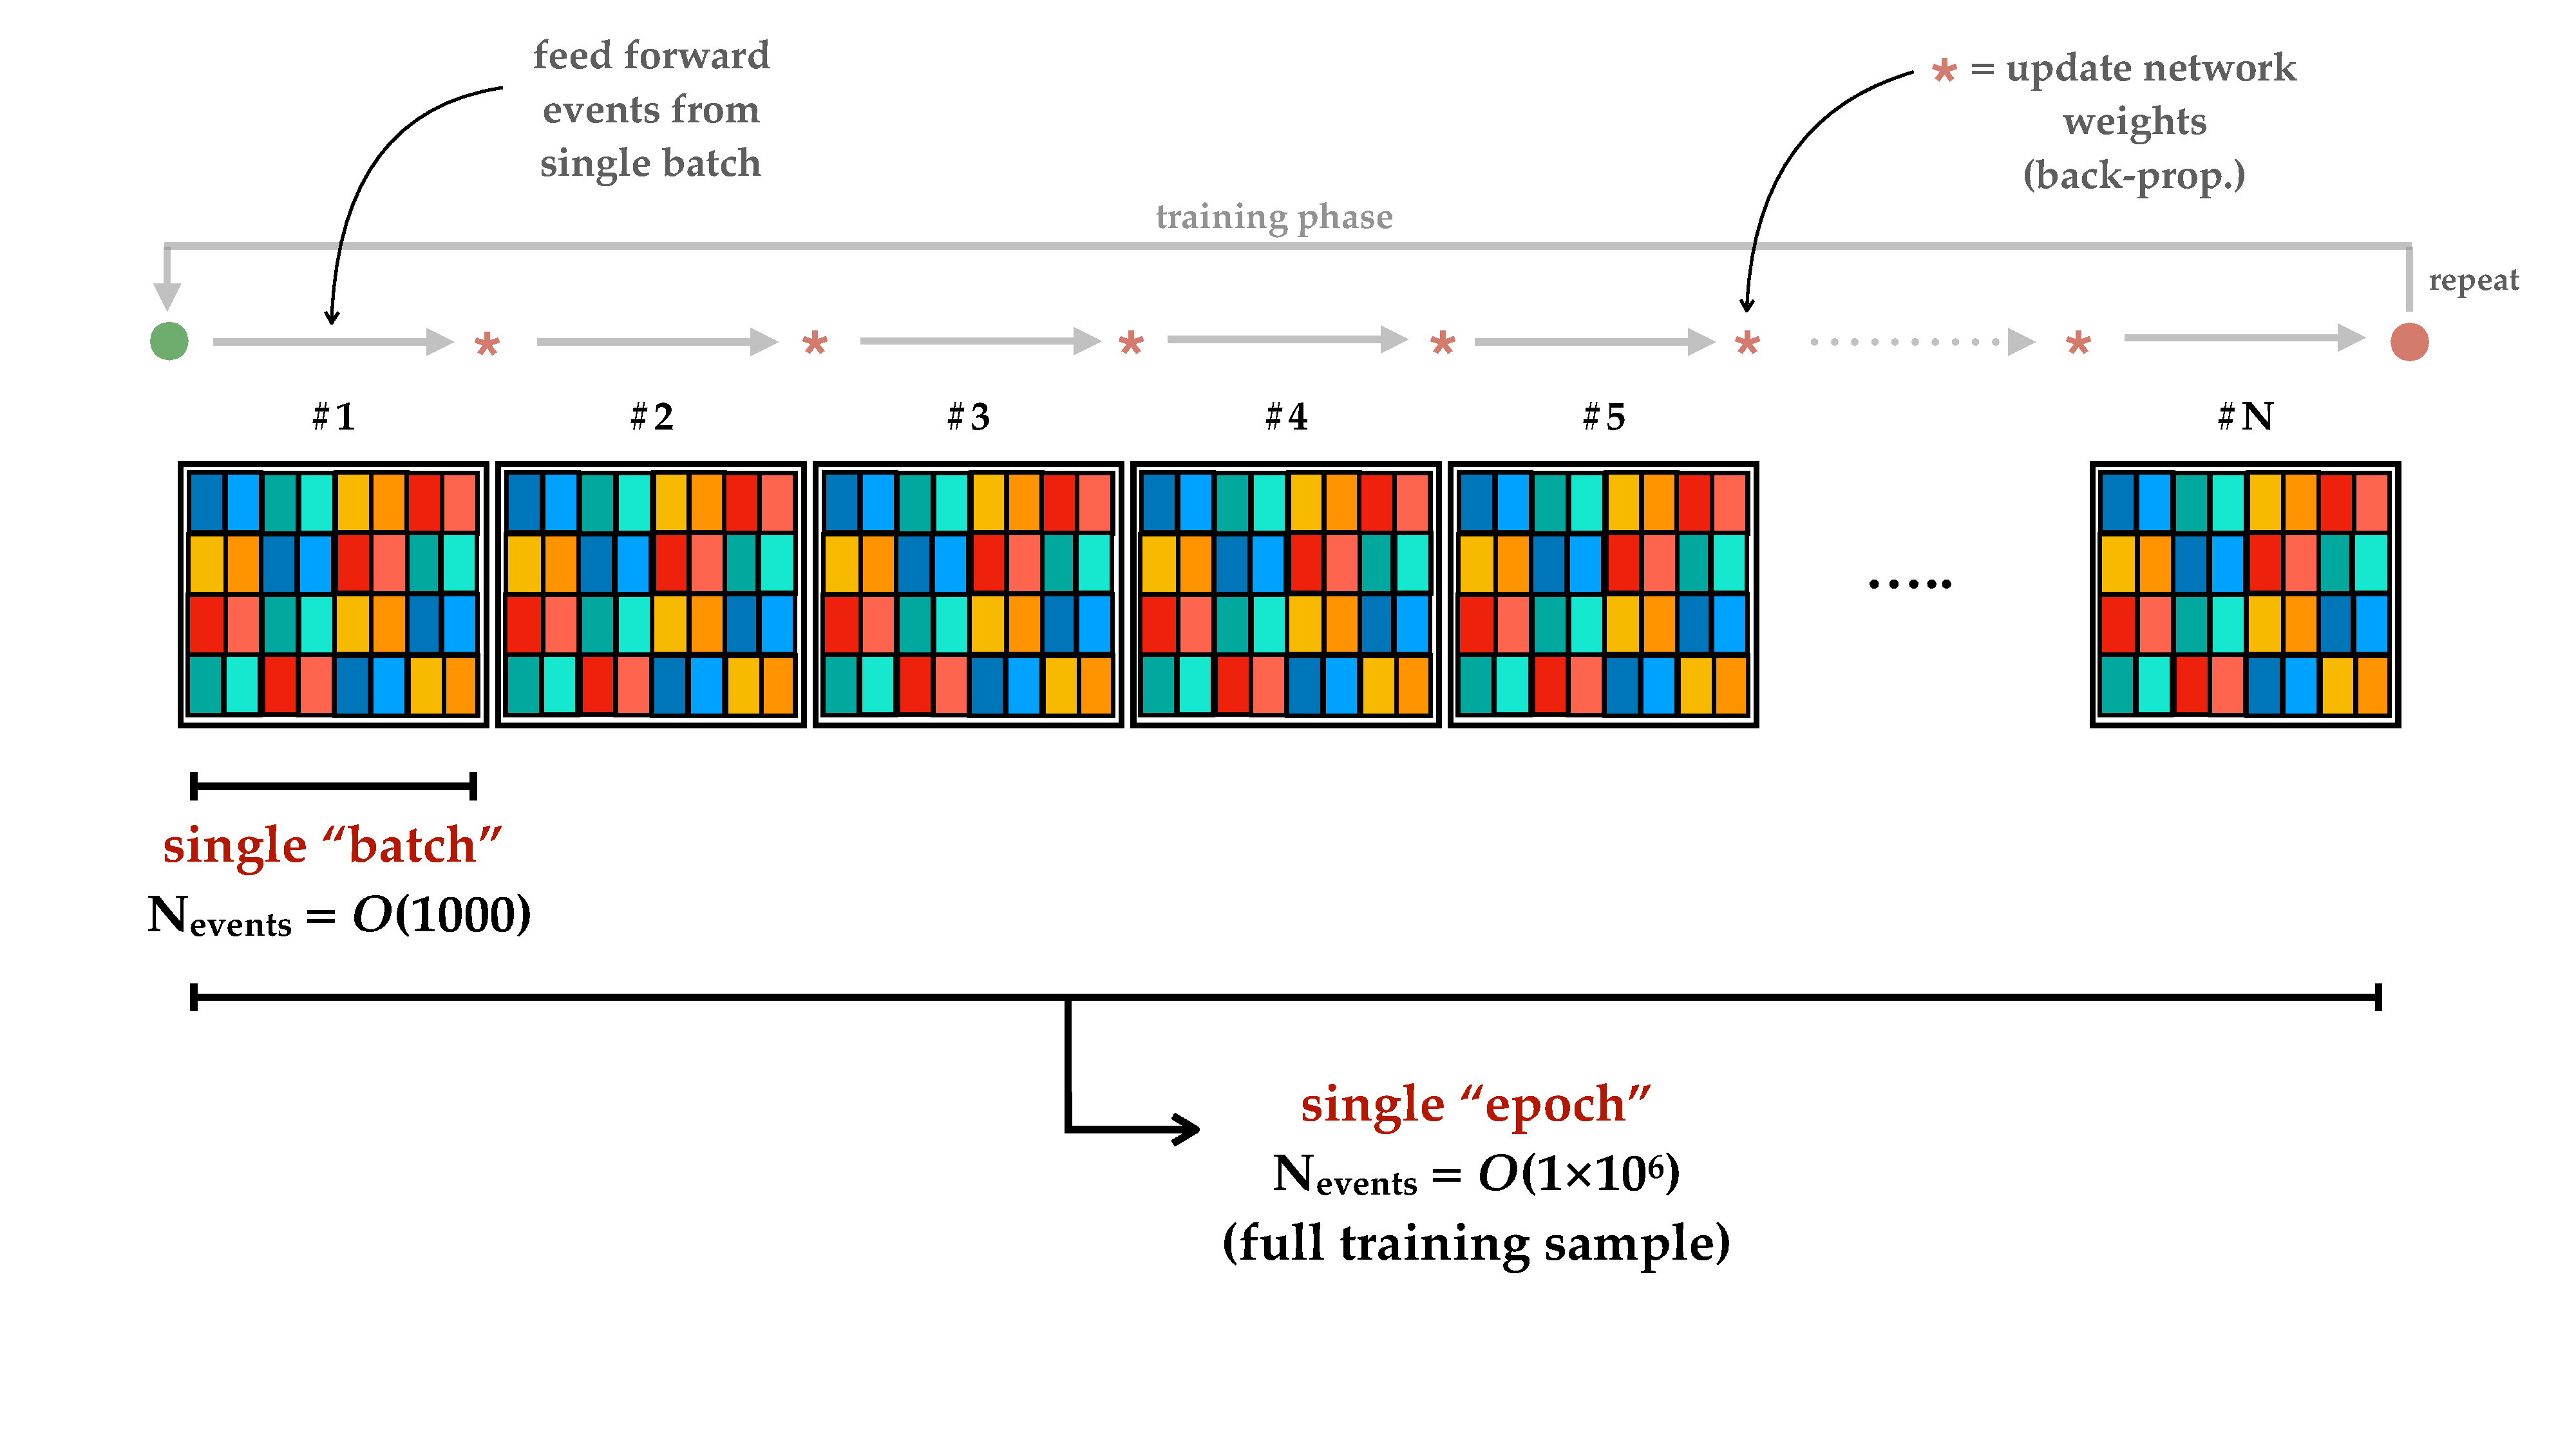
\includegraphics[width=1.0\textwidth]{figures/search_hh/mva/nn_batchesPDF}
        \caption{
            A neural network training sample is broken into many sub-samples referred to as `batches'.
            In the training phase of the neural network, the network parameters (weights and biases)
            are only updated after each batch is fed into the network.
            A training `epoch' refers to the point in the training at which all of the events
            in the entire training sample have been fed forward through the network for training purposes.
            The size of each batch (i.e. the number of events that are in a batch), as well as the number
            epochs to train for, are configurable parameters that must be optimized.
            See Ref.~\cite{GoodFellowBook} for more information.
        }
        \label{fig:nn_batches}
    \end{center}
\end{figure}

\begin{figure}[!htb]
    \begin{center}
        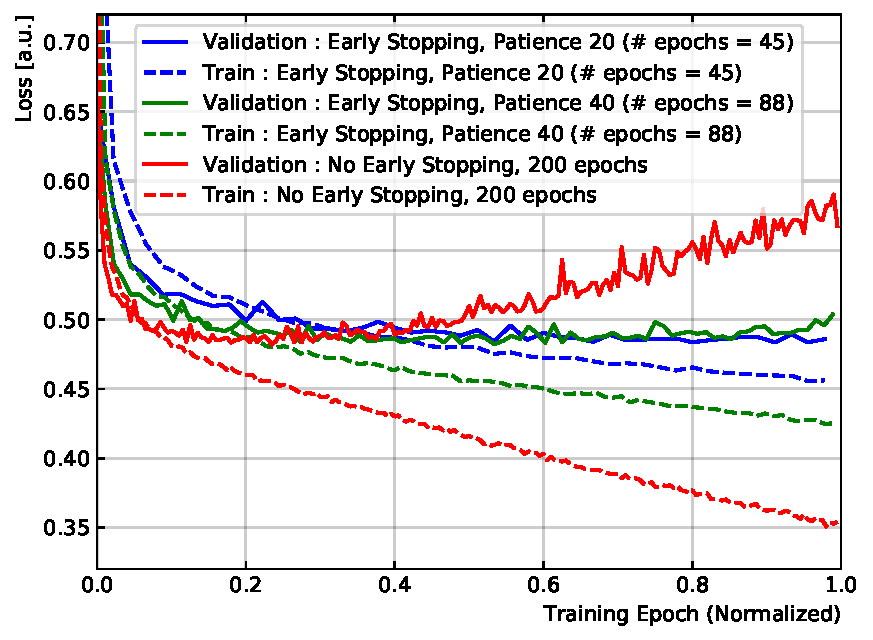
\includegraphics[width=0.48\textwidth]{figures/search_hh/mva/overtrain_check_loss}
        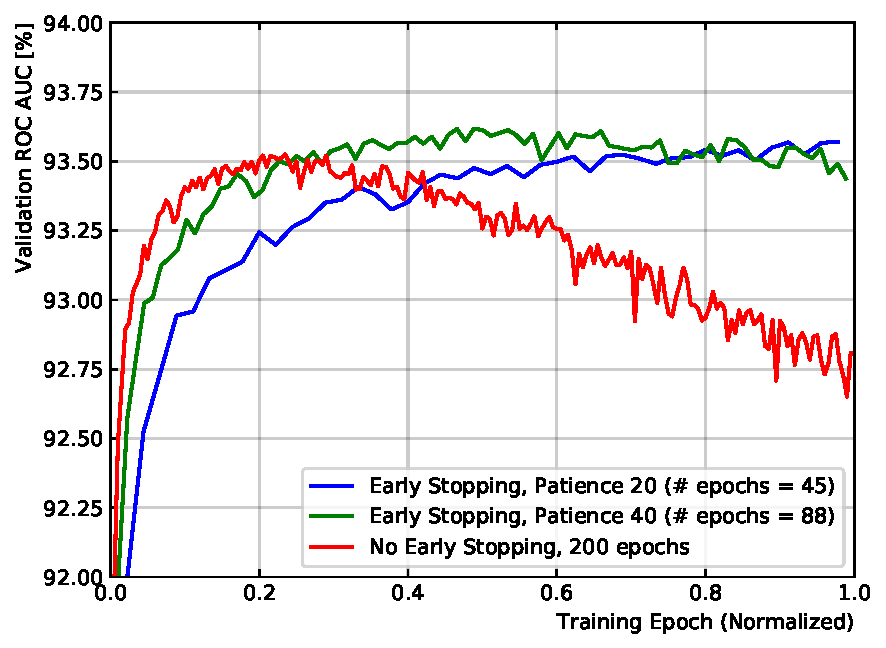
\includegraphics[width=0.48\textwidth]{figures/search_hh/mva/overtrain_check_roc_auc}
        \caption{
            \textit{\textbf{Left}}: The neural network loss as a function of the number of training epochs.
                The solid lines report the loss evaluated on the held-out validation sample of events,
                while the dashed lines report that evaluated using the sample of events used for training.
                The larger discrepancy observed between the validation and training loss observed in the
                cases where the training is allowed to proceed for a larger number of epochs indicate
                larger amounts of overtraining.
            \textit{\textbf{Right}}: Receiver operating characteristic area-under-the-curve (ROC AUC), evaluated using
                the held-out validation sample of events, as a function of the number of training epochs.
                Larger values of ROC AUC indicate better network classification performance.
                The drop in ROC AUC observed in the green and red curves are a result of increased levels
                of overtraining, resulting in the classifier being unable to generalize to data other than
                that used for training.
        }
        \label{fig:nn_epoch_overtrain}
    \end{center}
\end{figure}

%%%%%%%%%%%%%%%%%%%%%%%%%%%%%%%%%%%%%%%%%%%%%%%%%%%%%%%%%%%%%%%%%%%%%%%%%%%%%%%%%%%
%%%%%%%%%%%%%%%%%%%%%%%%%%%%%%%%%%%%%%%%%%%%%%%%%%%%%%%%%%%%%%%%%%%%%%%%%%%%%%%%%%%
%%%%%%%%%%%%%%%%%%%%%%%%%%%%%%%%%%%%%%%%%%%%%%%%%%%%%%%%%%%%%%%%%%%%%%%%%%%%%%%%%%%
%
% NN DISCRIMINANTS
%
%%%%%%%%%%%%%%%%%%%%%%%%%%%%%%%%%%%%%%%%%%%%%%%%%%%%%%%%%%%%%%%%%%%%%%%%%%%%%%%%%%%
%%%%%%%%%%%%%%%%%%%%%%%%%%%%%%%%%%%%%%%%%%%%%%%%%%%%%%%%%%%%%%%%%%%%%%%%%%%%%%%%%%%
%%%%%%%%%%%%%%%%%%%%%%%%%%%%%%%%%%%%%%%%%%%%%%%%%%%%%%%%%%%%%%%%%%%%%%%%%%%%%%%%%%%

\subsection{Classifier Discriminants}
\label{sec:nn_discriminants}

The multi-output classifier described in Section~\ref{sec:nn_arch} provides four outputs for each event
once provided an input feature vector.
In our case, the four outputs are taken to loosely represent the probabilities, or strengths, that the
set of inputs correspond to one of the four labels for which the classifier has been trained to distinguish.
We refer to these outputs, then, as \phh, \ptop, \pzsf, and \pztt
for the $hh$, Top, $Z\rightarrow \{ee,\mu\mu\}$, and $Z\rightarrow \tau\tau$ process labels, respectively.
Representative distributions for each of the $p_i$, for the corresponding signal and background processes,
are shown in Figure~\ref{fig:nn_disc_p}.

From the set of $p_i$, we build a set of four composite discriminants, each of which combines information
contain within them all.
These discriminants are log-ratio discriminants of the output scores, defined in Equation~\ref{eq:nn_disc_def}.
Representative distributions for each of the composite discriminants are shown in Figure~\ref{fig:nn_disc_d}.
The discriminant \dhh is the primary observable around which the SRs, CRs, and VRs are defined
in the present analysis.

\begin{align}
    d_Q = \ln \left( \frac{p_Q}{p_X + p_Y + p_Z} \right)
    \label{eq:nn_disc_def}
\end{align}

\begin{figure}[!htb]
    \begin{center}
        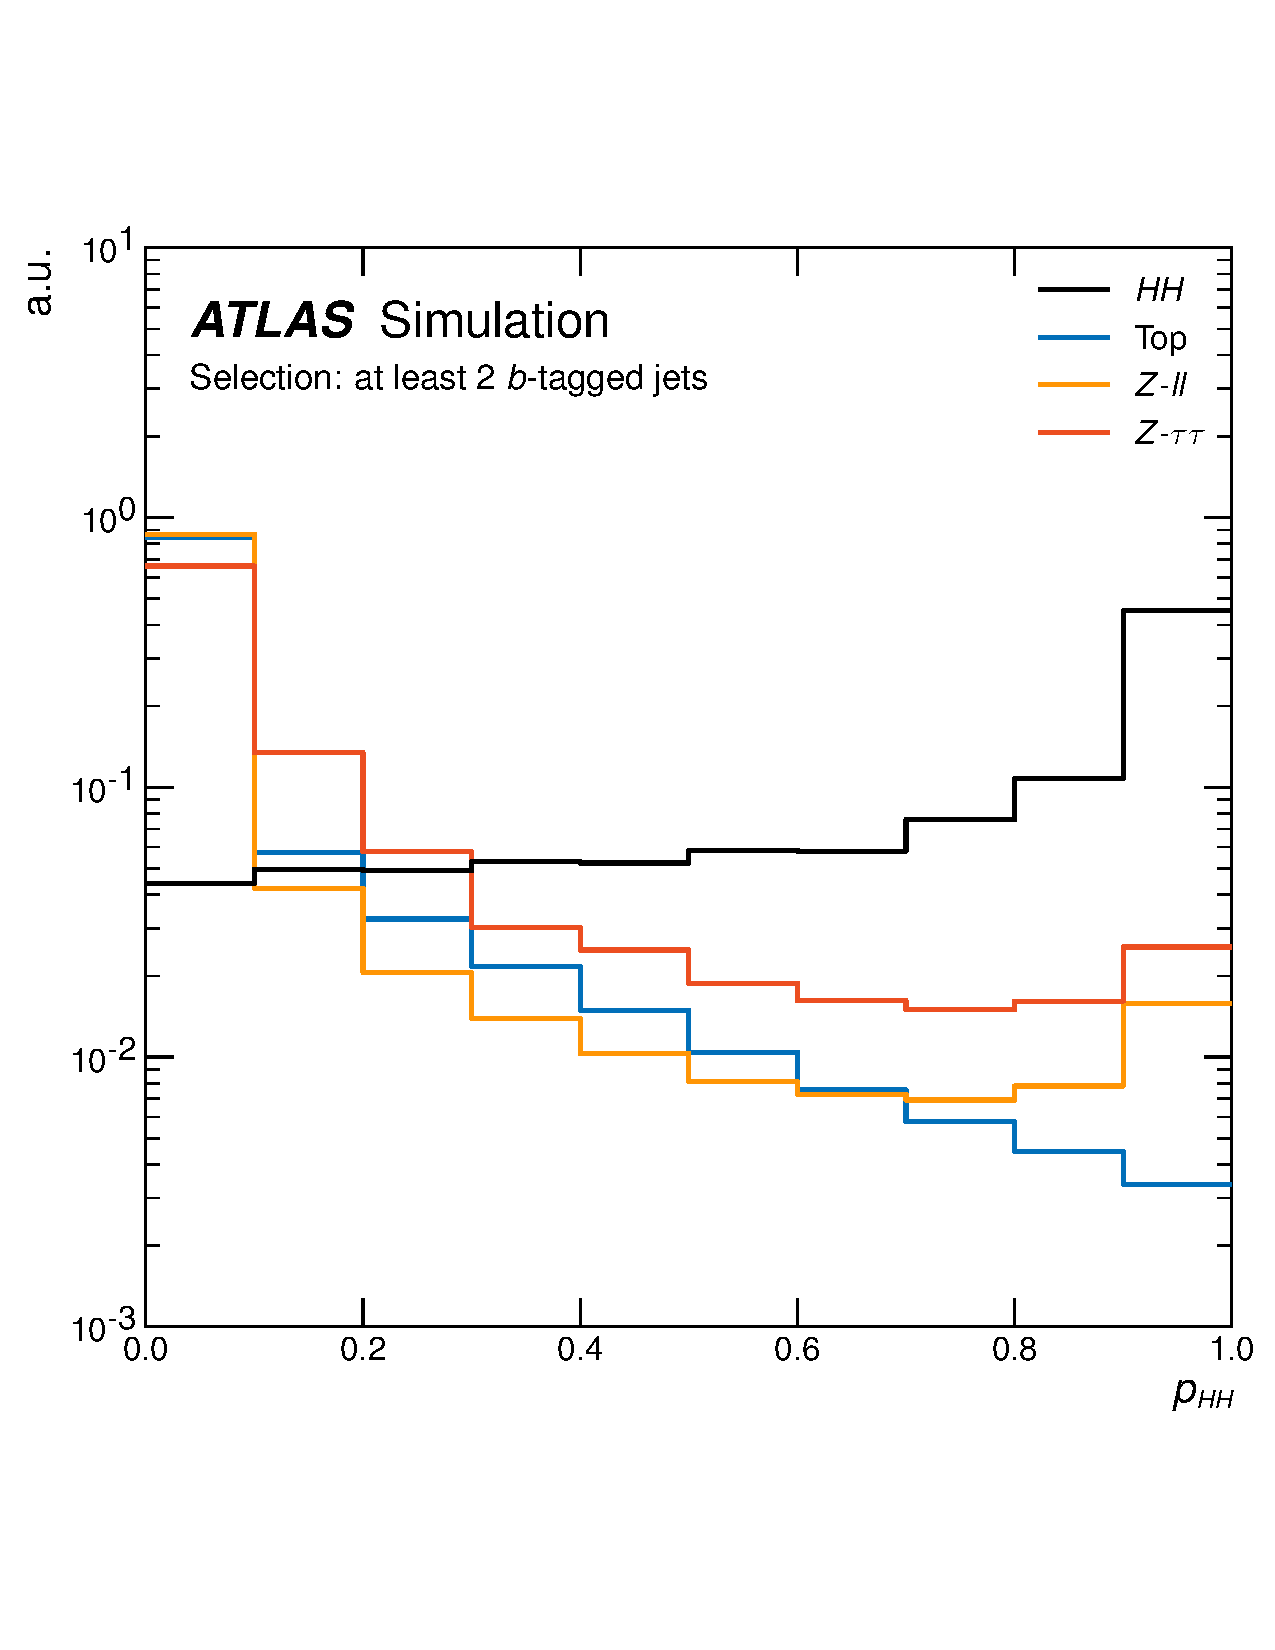
\includegraphics[width=0.48\textwidth]{figures/search_hh/nn_disc/pi_plot_NN_p_hh}
        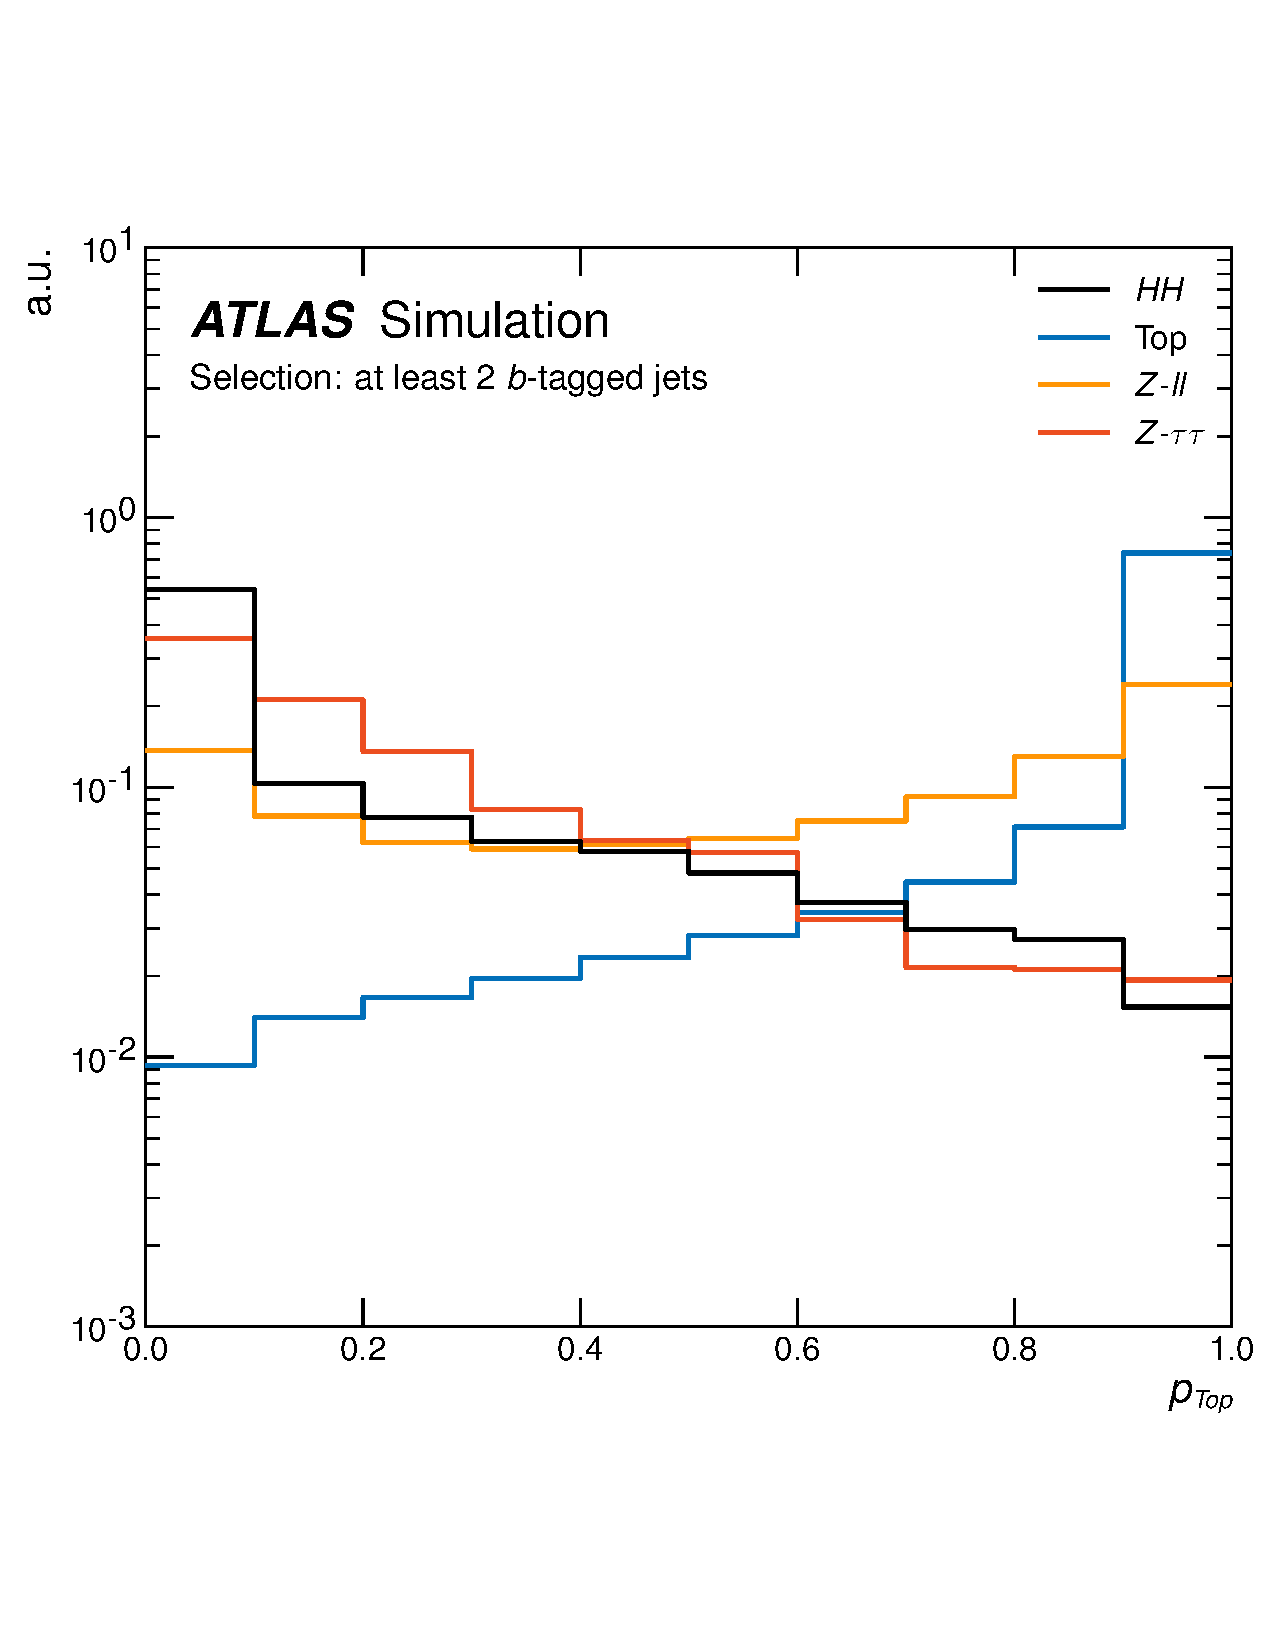
\includegraphics[width=0.48\textwidth]{figures/search_hh/nn_disc/pi_plot_NN_p_top}
        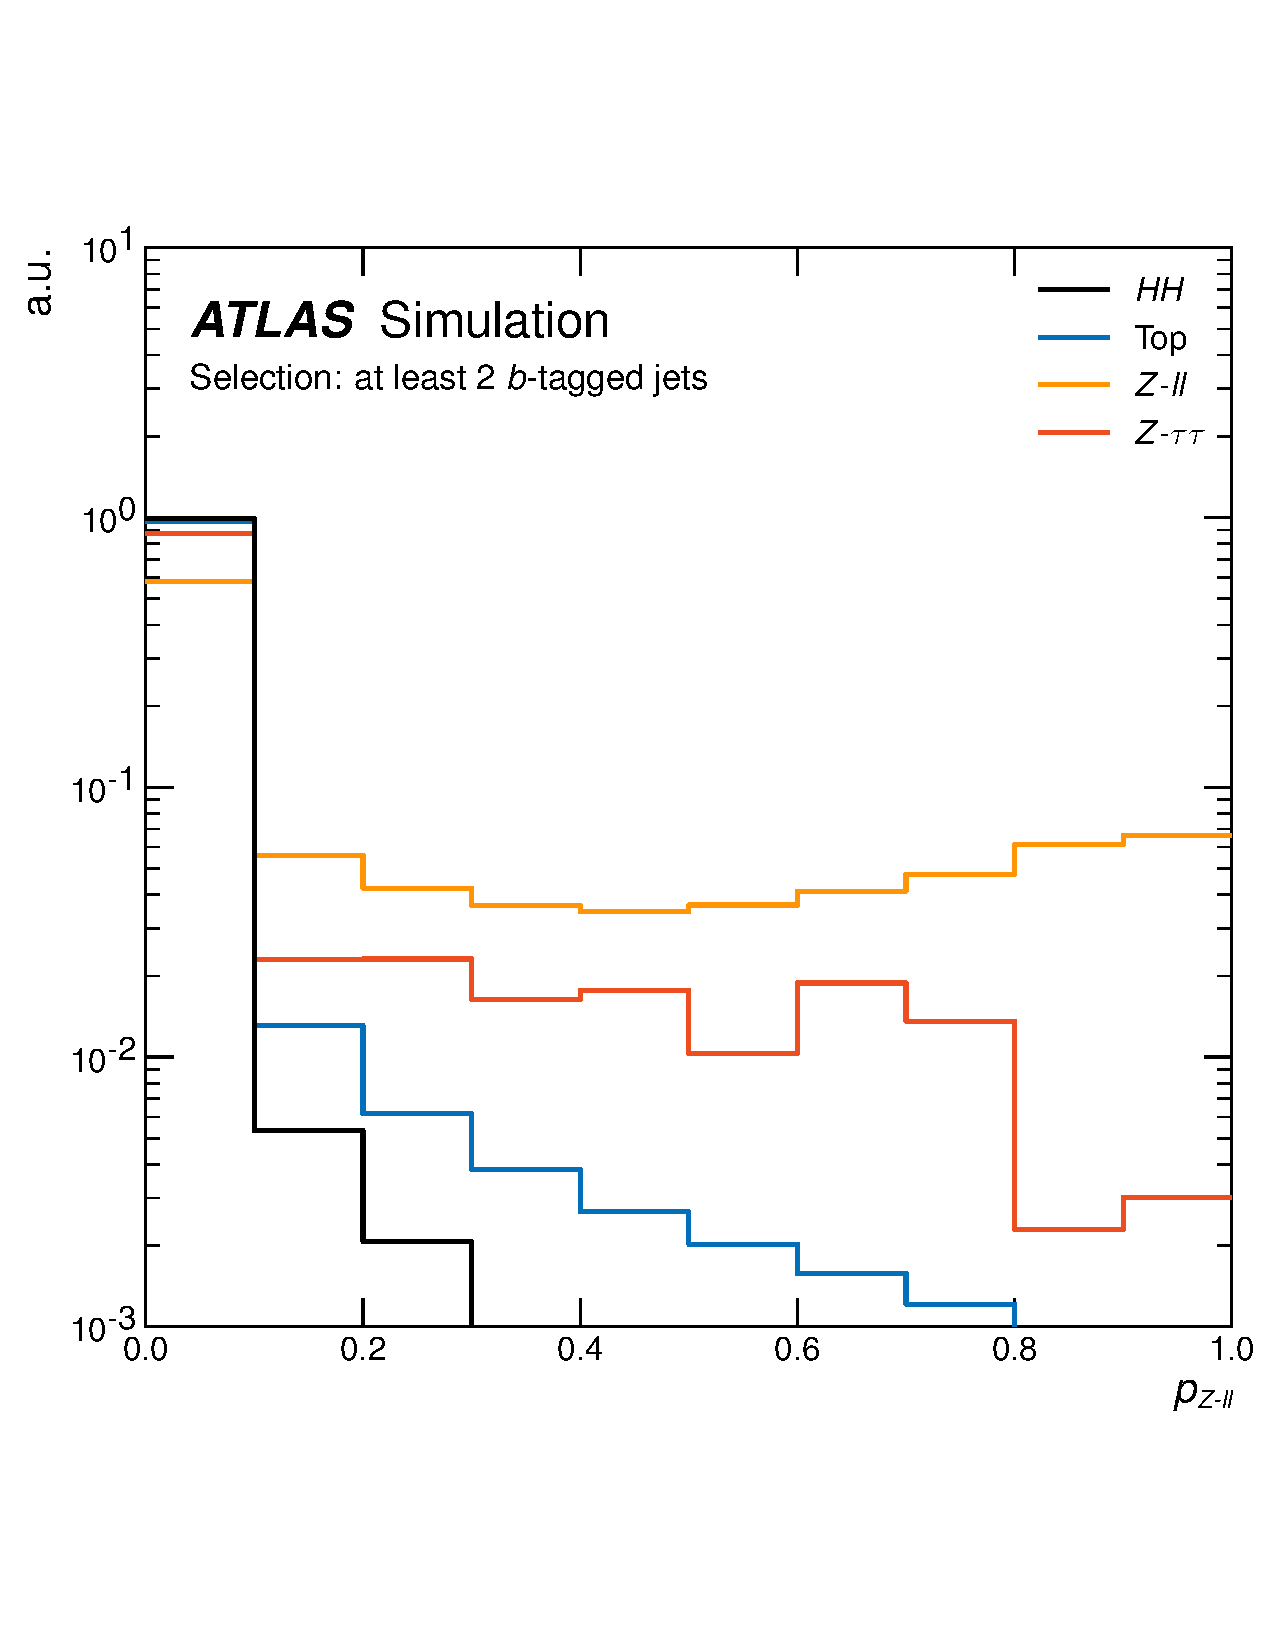
\includegraphics[width=0.48\textwidth]{figures/search_hh/nn_disc/pi_plot_NN_p_zsf}
        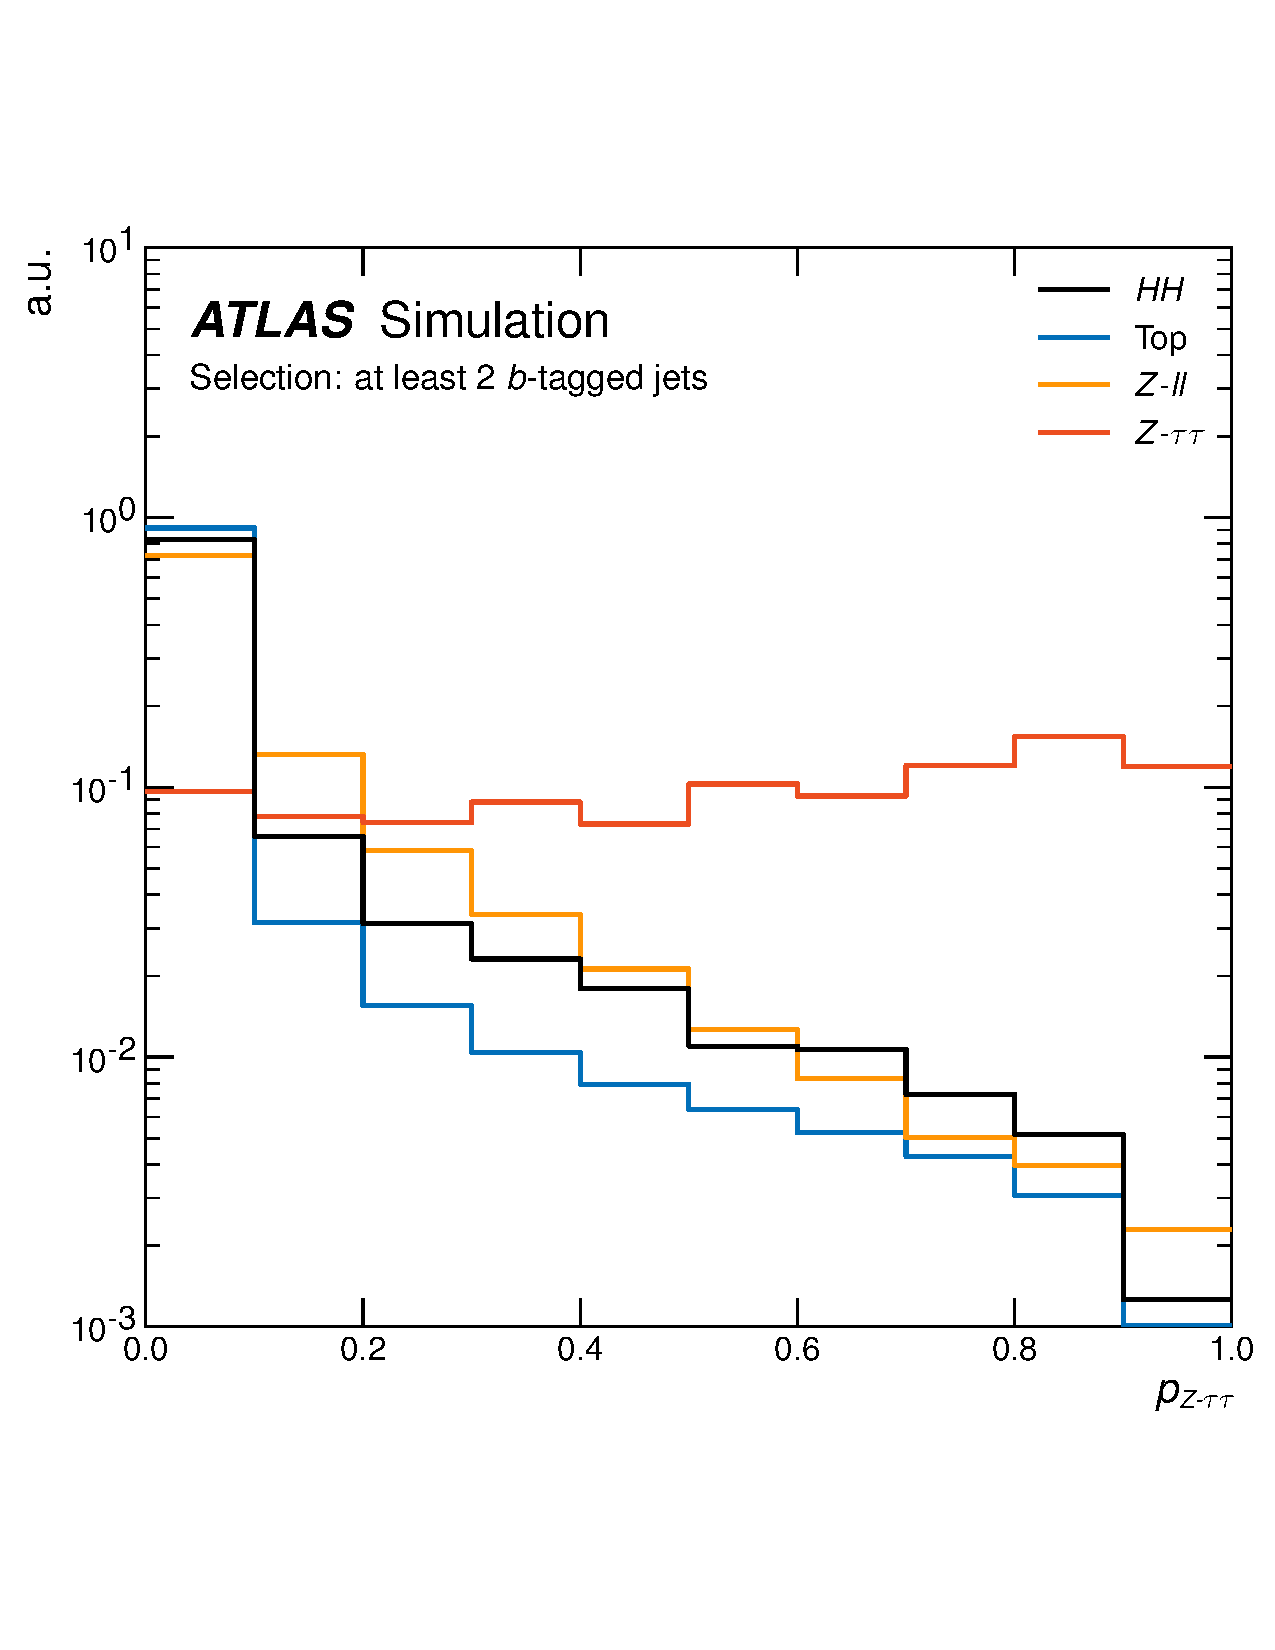
\includegraphics[width=0.48\textwidth]{figures/search_hh/nn_disc/pi_plot_NN_p_ztt}
        \caption{
            Normalized distributions of the four network outputs,
            shown for the dilepton
            $hh \rightarrow \bbww$ signal (black), Top (blue), $Z \rightarrow \{ee,\mu\mu\}$ (yellow),
            and $Z\rightarrow \tau\tau$ (orange) processes.
            From the top left and moving clock-wise: \phh, \ptop, \pztt, and \pzsf.
        }
        \label{fig:nn_disc_p}
    \end{center}
\end{figure}

\begin{figure}[!htb]
    \begin{center}
        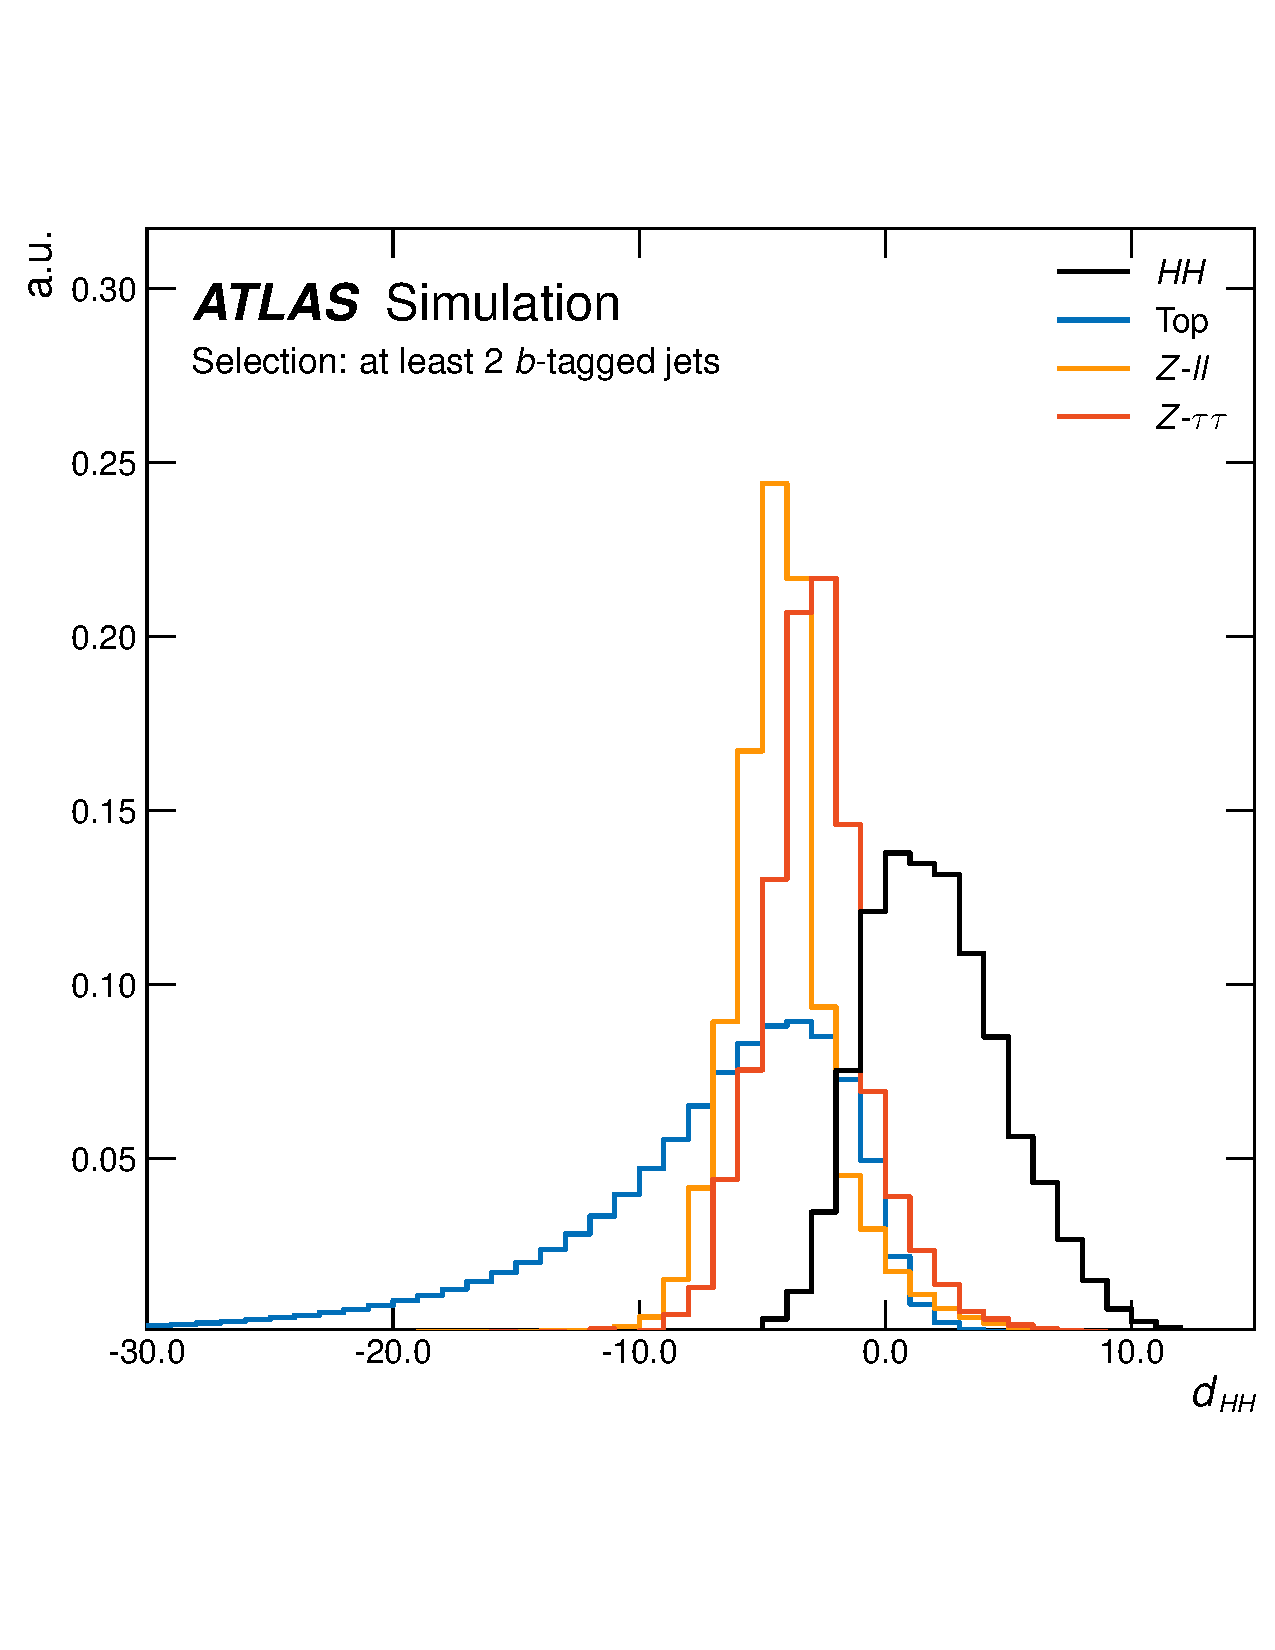
\includegraphics[width=0.48\textwidth]{figures/search_hh/nn_disc/pi_plot_NN_d_hh}
        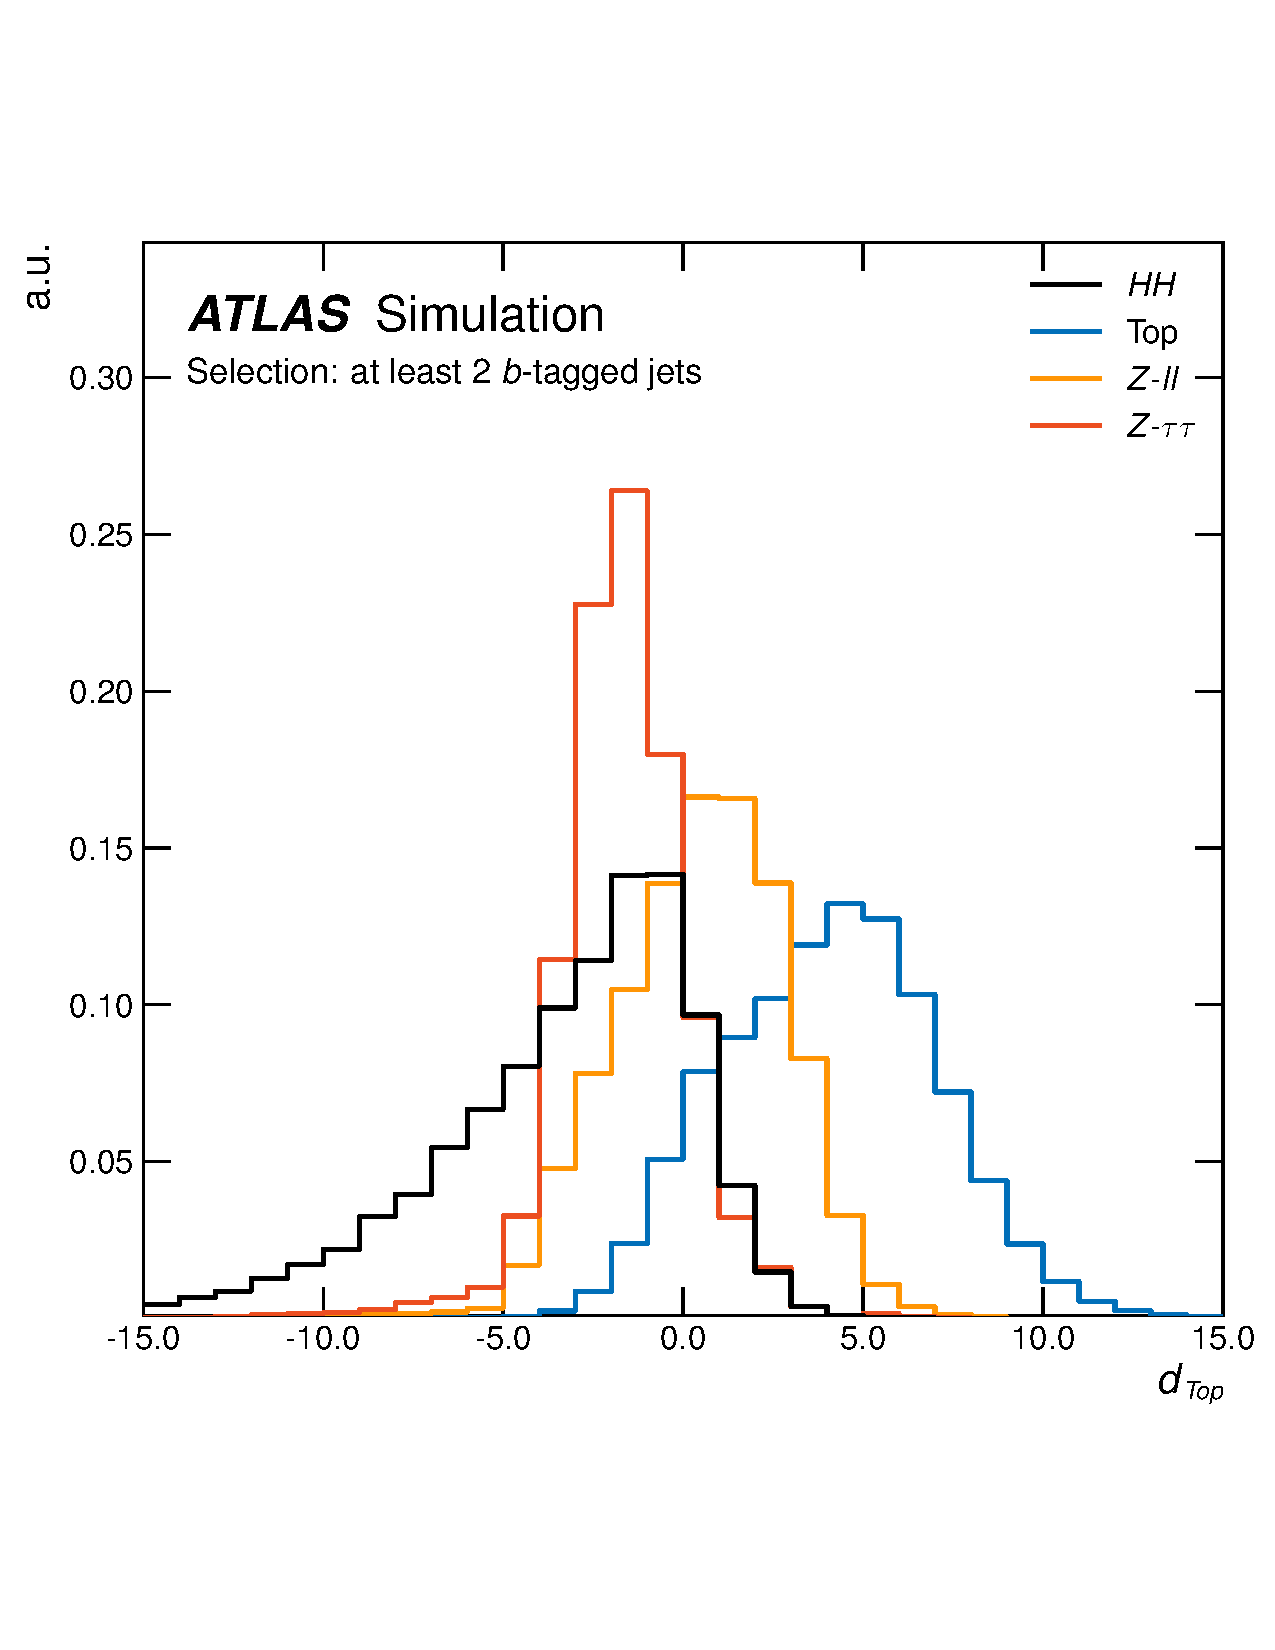
\includegraphics[width=0.48\textwidth]{figures/search_hh/nn_disc/pi_plot_NN_d_top}
        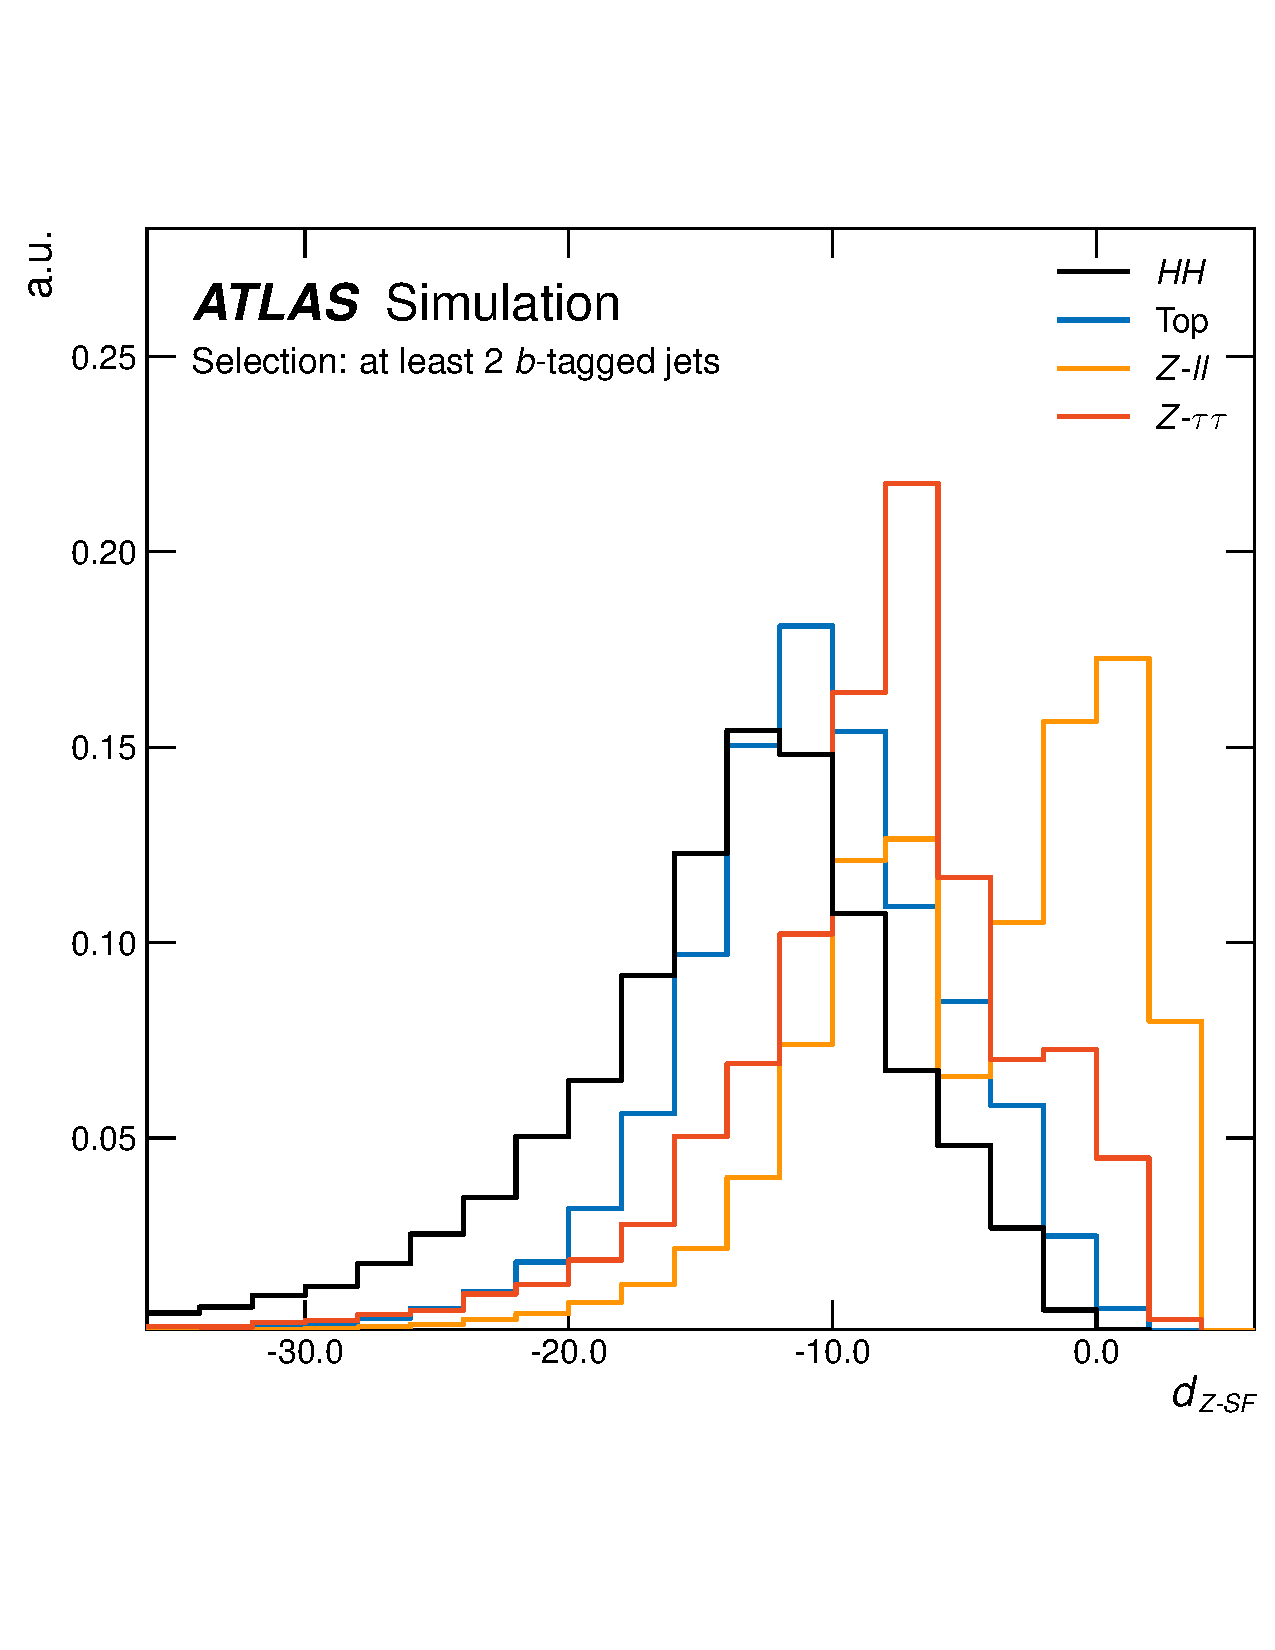
\includegraphics[width=0.48\textwidth]{figures/search_hh/nn_disc/pi_plot_NN_d_zsf}
        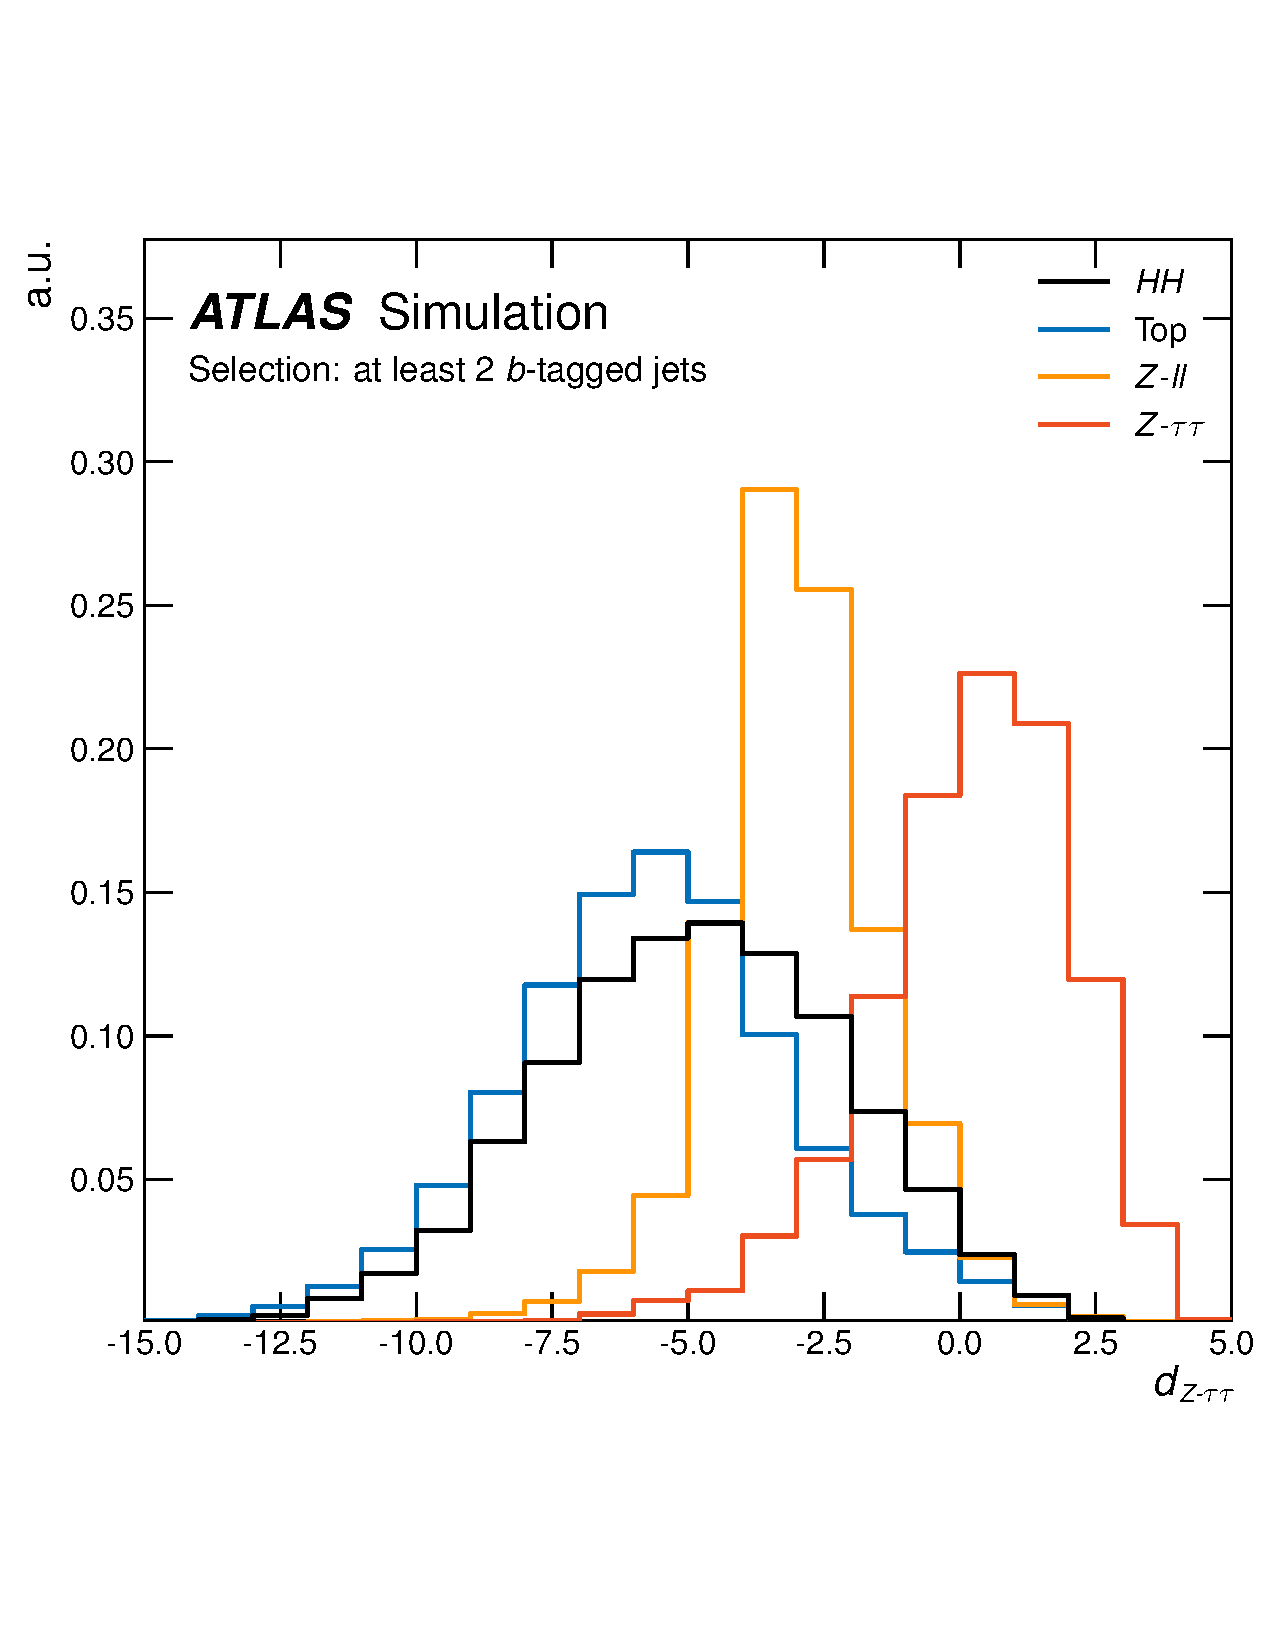
\includegraphics[width=0.48\textwidth]{figures/search_hh/nn_disc/pi_plot_NN_d_ztt}
        \caption{
            Normalized distributions of the four composite discriminants,
            shown for the dilepton
            $hh \rightarrow \bbww$ signal (black), Top (blue), $Z \rightarrow \{ee,\mu\mu\}$ (yellow),
            and $Z\rightarrow \tau\tau$ (orange) processes.
            From the top left and moving clock-wise: \dhh, \dtop, \dztt, and \dzsf.
        }
        \label{fig:nn_disc_d}
    \end{center}
\end{figure}

%%%%%%%%%%%%%%%%%%%%%%%%%%%%%%%%%%%%%%%%%%%%%%%%%%%%%%%%%%%%%%%%%%%%%%%%%%%%%%%%%%%
%%%%%%%%%%%%%%%%%%%%%%%%%%%%%%%%%%%%%%%%%%%%%%%%%%%%%%%%%%%%%%%%%%%%%%%%%%%%%%%%%%%
%%%%%%%%%%%%%%%%%%%%%%%%%%%%%%%%%%%%%%%%%%%%%%%%%%%%%%%%%%%%%%%%%%%%%%%%%%%%%%%%%%%
%
% SR DEFINITION
%
%%%%%%%%%%%%%%%%%%%%%%%%%%%%%%%%%%%%%%%%%%%%%%%%%%%%%%%%%%%%%%%%%%%%%%%%%%%%%%%%%%%
%%%%%%%%%%%%%%%%%%%%%%%%%%%%%%%%%%%%%%%%%%%%%%%%%%%%%%%%%%%%%%%%%%%%%%%%%%%%%%%%%%%
%%%%%%%%%%%%%%%%%%%%%%%%%%%%%%%%%%%%%%%%%%%%%%%%%%%%%%%%%%%%%%%%%%%%%%%%%%%%%%%%%%%

\subsection{Signal Region Definition}
\label{sec:hh_sr_def}

The definitions of the SRs, SR-SF and SR-DF, targeting the dilepton $hh \rightarrow \bbww$ signal process are tabulated
in Table~\ref{tab:hh_sr_def} and are as follows.
The dominant expected backgrounds in the analysis are those for which separate output labels
have been defined in the construction of the neural network classifier described in the previous sections:
SM top-quark processes (\ttbar~and single-top $Wt$) and $Z$+jets processes.
The top-quark processes are flavor symmetric, however the $Z$+jets processes tend primarily to populate
only the same-flavor dilepton final states, with a smaller component in the different-flavor dilepton
final state due to the leptonic $\tau$ decays in the $Z\rightarrow \tau \tau$ process.
For this reason, we define two classes of SR: one requiring SF dilepton events and the
other requiring DF dilepton events.
The SR events are additionally required to have at least two $b$-tagged jets, with
the invariant mass of the two leading $b$-tagged jets having an invariant mass consistent with the
mass of the Higgs boson, $m_{bb} \in [110, 140]$ GeV.
Taking advantage of the lepton correlations, illustrated by Figure~\ref{fig:hh_kin_1},
we further require that the dilepton invariant mass of the SR events be relatively low: $m_{\ell \ell} < 60$ GeV.
This requirement on $m_{\ell \ell}$ effectively acts to remove the majority of background events
arising from $Z$-boson processes.

The SR definitions further rely on placing a cut on the $d_{hh}$ discriminant.
The specific choice of cut, in both SR-SF and SR-DF, are determined by computing the expected 95\% CL cross-section upper-limit
with the selections described in the previous paragraph applied while scanning over varying selections
made on the $d_{hh}$ discriminant.
The cut thresholds on the $d_{hh}$ discriminant in both SR-SF and SR-DF that minimize the cross-section
upper-limit value are chosen as the final values to define SR-SF and SR-DF, and are indicated in Table~\ref{tab:hh_sr_def}.


\begin{table}[!htb]
    \begin{center}
        \caption{
            SRs for the search for the dilepton $hh \rightarrow \bbww$ process.
        }
        \label{tab:hh_sr_def}
        \begin{tabular}{l | c c}
        \hline
        \hline
                & \multicolumn{2}{c}{\textbf{Region}} \\
            \cline{2-3}
            \textbf{Observable} & \textbf{SR-SF} & \textbf{SR-DF} \\
            \hline
            Dilepton Flavor & $ee$ or $\mu\mu$ & $e\mu$ or $\mu e$ \\
            $b$-tagged jet multiplicity & $\ge 2$ & $\ge 2 $ \\
            $bb$-system invariant mass, $m_{bb}$ [GeV] & $\in [110, 140]$ & $\in [110, 140]$ \\
            Dilepton invariant mass, $m_{\ell \ell}$ [GeV] & $<60$ & $<60$ \\
            \dhh & $>5.45$ & $>5.55$ \\
        \hline
        \hline
        \end{tabular}
    \end{center}
\end{table}

\section{Estimation of the Standard Model Backgrounds}
\label{sec:stop_background_estimate}

In this section, we describe the methods used for the estimation of the SM background
contamination in the SRs.
By Table~\ref{tab:stop_exp_sr_yield}, it can be seen that the expected SM background
contamination to the SRs in the \bWN search is primarily composed of events
from the \ttbar~and diboson processes.
Given that these are the dominant backgrounds for the analysis, their estimation is performed
using the control region method, described in Section~\ref{sec:control_region_method}.
That is, dedicated CRs and VRs are defined for each of the two processes in order
to provide a normalisation correction for their MC prediction in the SRs.
All other background processes, being subdominant, have their predicted contribution
to the SR background taken directly from the MC simulation.
The estimation of the contribution of sources leading to fake and non-prompt leptons
is performed using the Matrix Method, described in Section~\ref{sec:matrix_method}.

Sections~\ref{sec:stop_ttbar_estimate} and \ref{sec:stop_vv_estimate} describe
the background estimate for the \ttbar~and diboson processes, respectively.

The CR and VR definitions for both the \ttbar~and diboson background are based on the
SR definitions given in the previous section.
The CRs are defined primarily by inverting the two-dimensional selection
made in the $(\cosb, \dpb)$-plane, and maintaining similar selections as in the SRs for the other variables.
The VRs, on the other hand, are defined by inverting the selections on the non-angular variables relative to those
made in the SRs.

\begin{figure}[!htb]
    \begin{center}
        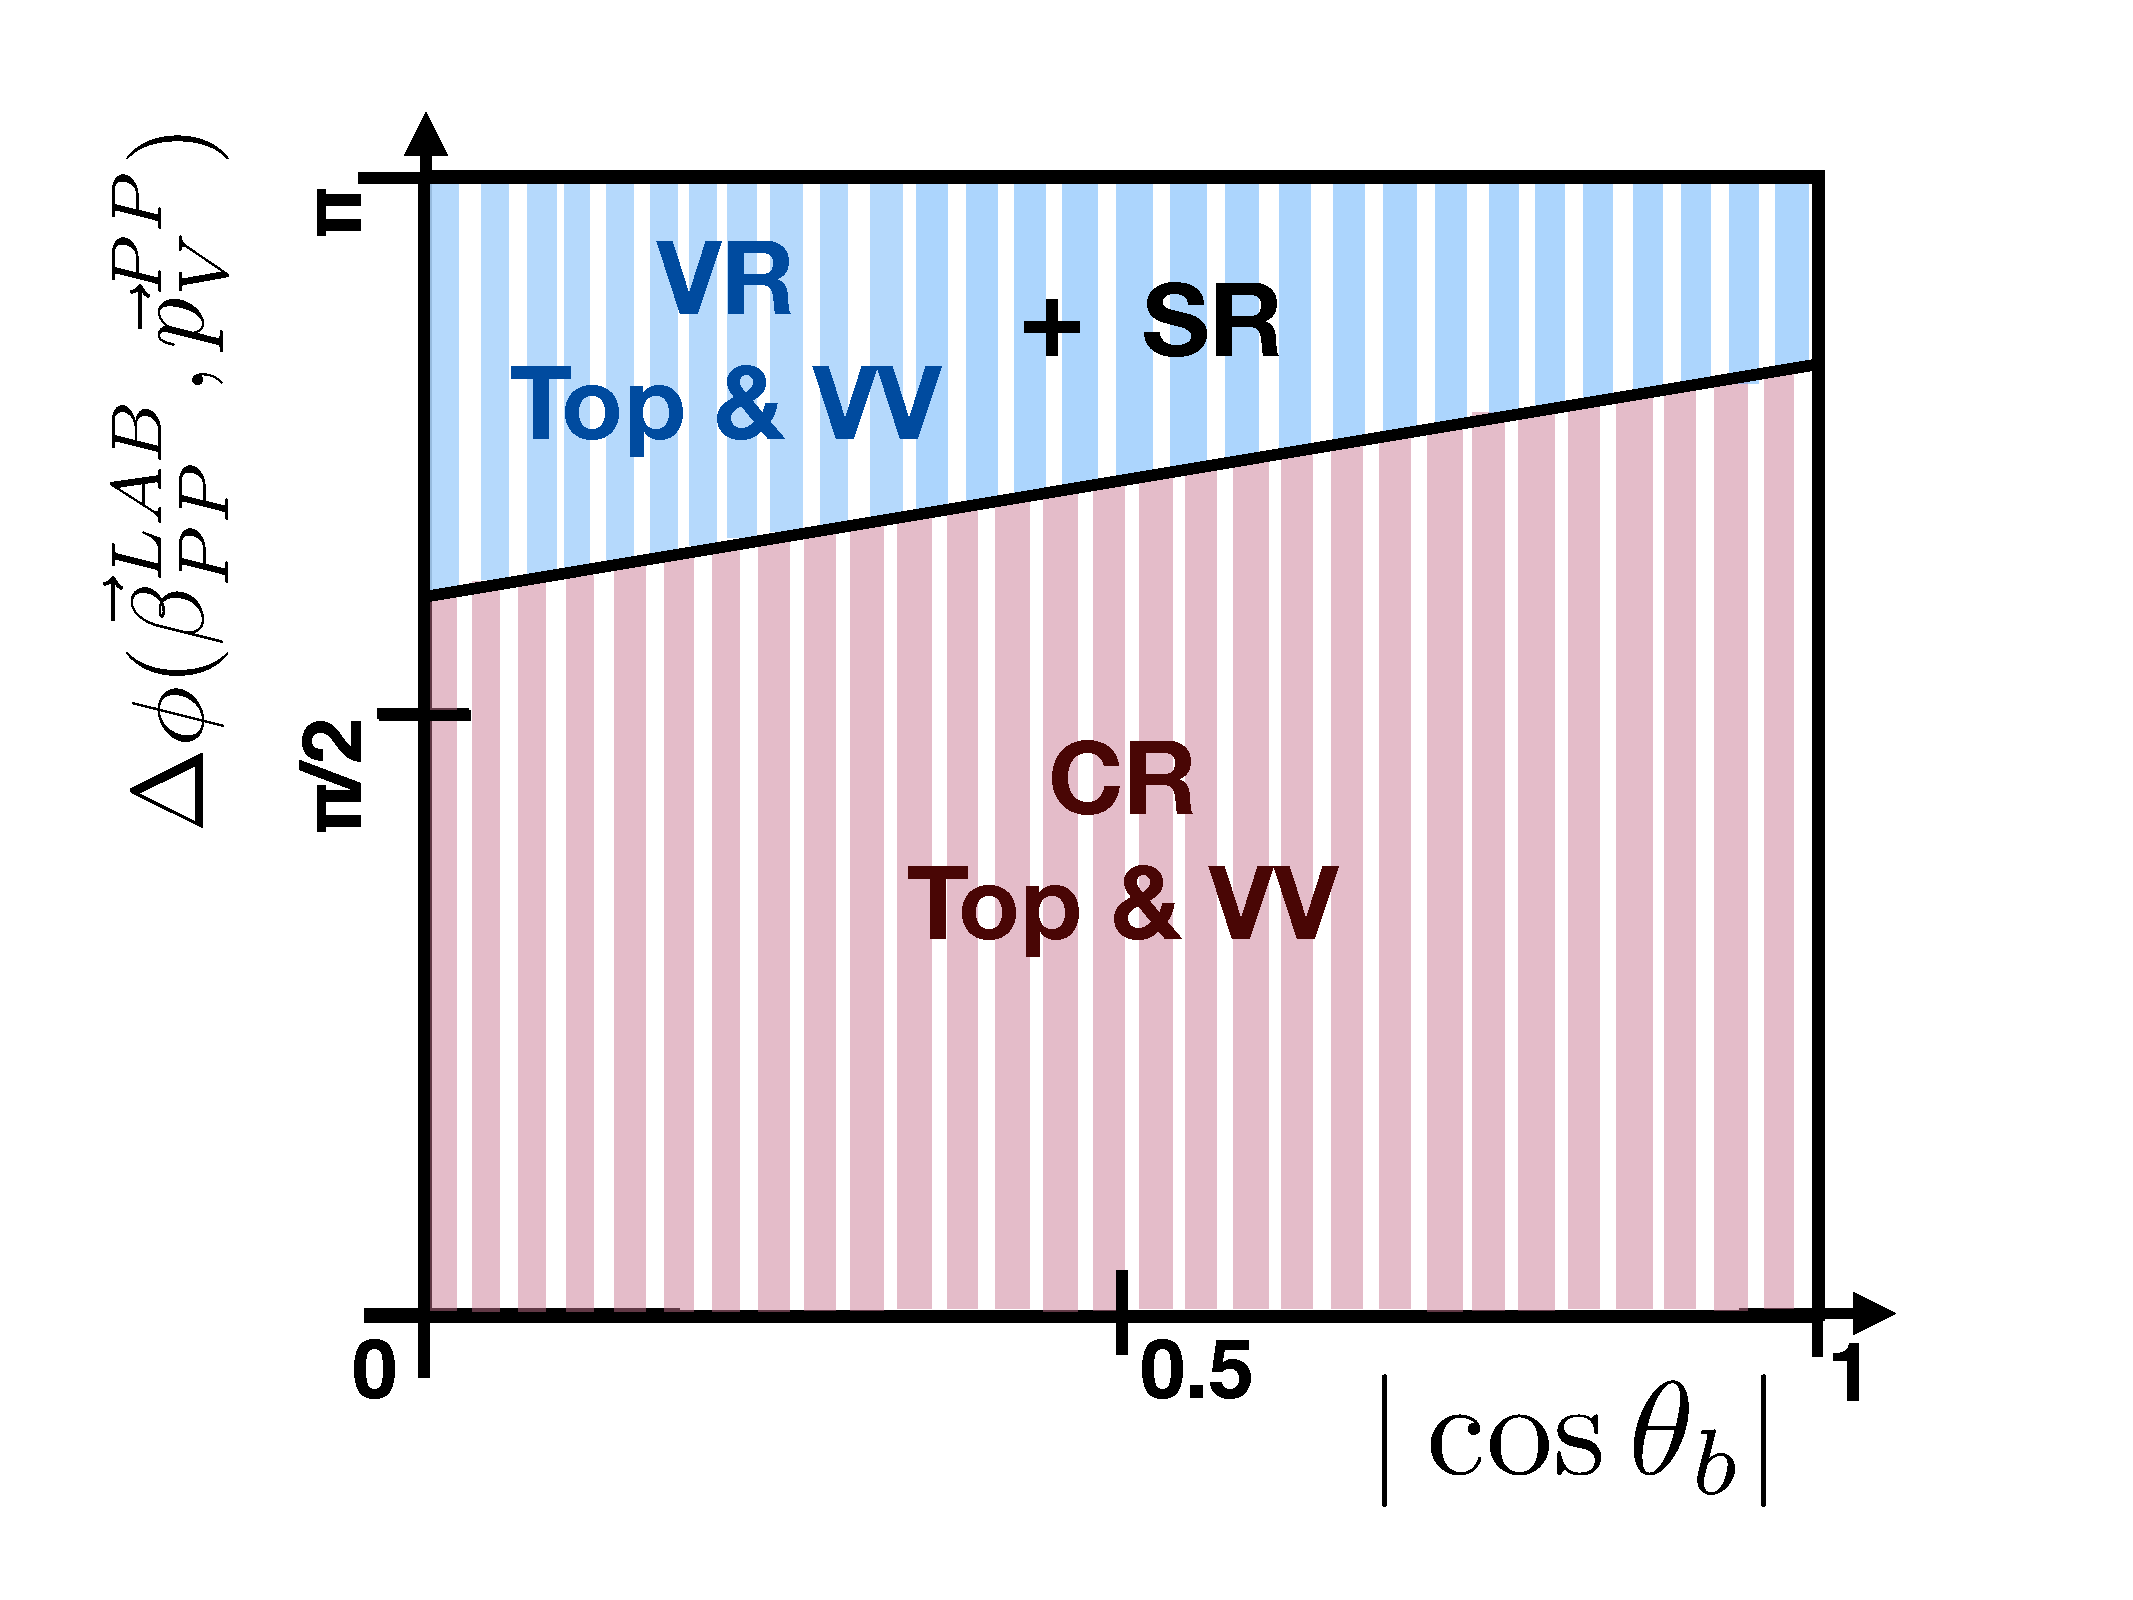
\includegraphics[width=0.7\textwidth]{figures/search_stop2l/bkg_est/crvrmotivation}
        \caption{
            Illustration of the CR and VR strategy used in the \bWN search.
            The defining characteristic for the definition of these regions is
            based on the region in the $(\cosb, \dpb)$-plane that they select.
            The CR inverts the requirements on these quantities relative to the SRs,
            while the VR has the same requirements as in the SRs but inverts
            selections made on the other observables.
        }
        \label{fig:stop_crvr_motivation}
    \end{center}
\end{figure}

\FloatBarrier
%%%%%%%%%%%%%%%%%%%%%%%%%%%%%%%%%%%%%%%%%%%%%%%%%%%%%%%%%%%%%%%%%%%%%%%%%%%%%%%%%%%%%%%%%%%%
%%%%%%%%%%%%%%%%%%%%%%%%%%%%%%%%%%%%%%%%%%%%%%%%%%%%%%%%%%%%%%%%%%%%%%%%%%%%%%%%%%%%%%%%%%%%
%%%%%%%%%%%%%%%%%%%%%%%%%%%%%%%%%%%%%%%%%%%%%%%%%%%%%%%%%%%%%%%%%%%%%%%%%%%%%%%%%%%%%%%%%%%%
%
% TOP BKG
%
%%%%%%%%%%%%%%%%%%%%%%%%%%%%%%%%%%%%%%%%%%%%%%%%%%%%%%%%%%%%%%%%%%%%%%%%%%%%%%%%%%%%%%%%%%%%
%%%%%%%%%%%%%%%%%%%%%%%%%%%%%%%%%%%%%%%%%%%%%%%%%%%%%%%%%%%%%%%%%%%%%%%%%%%%%%%%%%%%%%%%%%%%
%%%%%%%%%%%%%%%%%%%%%%%%%%%%%%%%%%%%%%%%%%%%%%%%%%%%%%%%%%%%%%%%%%%%%%%%%%%%%%%%%%%%%%%%%%%%

\subsection{Top-quark pair production}
\label{sec:stop_ttbar_estimate}

The CRs and VRs designed to derive and validate the semi-data-driven
normalisation correction factor for the \ttbar~background process are called
CR-Top and VR-Top, respectively, and are defined in Table~\ref{tab:stop_top_crvr}.
The strategy for the CR and VR selections in the $(\cosb, \dpb)$ plane are described
in the previous section.
Several of the selections on the kinematic quantities relative to those in the SRs (c.f. Table~\ref{tab:stop_sr_def})
are relaxed.
In both CR-Top and VR-Top, the \mdr requirement is relaxed to $\mdr > 80$\,GeV and the requirement on the
\gaminv quantity is removed.
In VR-Top, the \rpt requirement is inverted relative to that used in the SRs.
Given that the \ttbar~background is flavor symmetric, only different-flavor events
are allowed to populate CR-Top and VR-Top, in order to avoid contamination from $Z$-boson processes.
As a result, no additional requirement on $m_{\ell\ell}$ is made in these regions.
For increased purity, CR-Top requires that there be at least one $b$-tagged jet,
while VR-Top applies a veto in order to be orthogonal to CR-Top.

VR-Top is defined to have zero $b$-tagged jets, while CR-Top requires at least one.
In dedicated studies, it has been verified that the \ttbar~normalisation correction derived
in the $b$-jet rich region CR-Top is well extrapolated to separate validation regions, and is rather
independent of the $b$-tagged jet multiplicity.
This gives confidence that VR-Top can be used as an appropriate check on the \ttbar~normalisation
correct factor and that it's extrapolation to the SRs, which have differing requirements on the
$b$-tagged jet multiplicity, is reasonable.

Distributions of several key observables in CR-Top are shown in Figures~\ref{fig:crt_0}-\ref{fig:crt_1}.

\begin{table}[!htb]
    \begin{center}
        \begin{scriptsize}
        \caption{
            Definitions of the CR and VR for the \ttbar~background process for the
            \bWN search.
        }
        \label{tab:stop_top_crvr}
        \begin{tabular}{l | c c}
            \hline
            \hline
                & \multicolumn{2}{c}{\textbf{Regions}} \\
            \hline
            \textbf{Variable} & \textbf{CR-Top} & \textbf{VR-Top} \\
            \hline
            Dilepton Flavor & DF & DF \\
            $m_{\ell\ell}$ [GeV]    & no req. & no req. \\
            Lead lepton \pT~[GeV] & $>25$ & $>25$ \\
            Sub-lead lepton \pT~[GeV] & $>20$ & $>20$ \\
            $b$-tagged jet multiplicity & $>0$ & Exactly 0 \\
            \mdr [GeV] & $>80$ & $>80$ \\
            \rpt & $>0.7$ & $<0.7$ \\
            \gaminv & no req. & no req. \\
            $(\cosb, \dpb)$ & \multicolumn{1}{c}{\small{$\dpb < 0.9 \times | \cosb | + 1.6$}} & \multicolumn{1}{c}{\small{$\dpb> 0.9 \times | \cosb | + 1.6$}} \\
            \hline
            \hline
        \end{tabular}
        \end{scriptsize}
    \end{center}
\end{table}

\subsubsection{Kinematic Distributions in CR-Top}

\begin{figure}[!htb]
    \begin{center}
        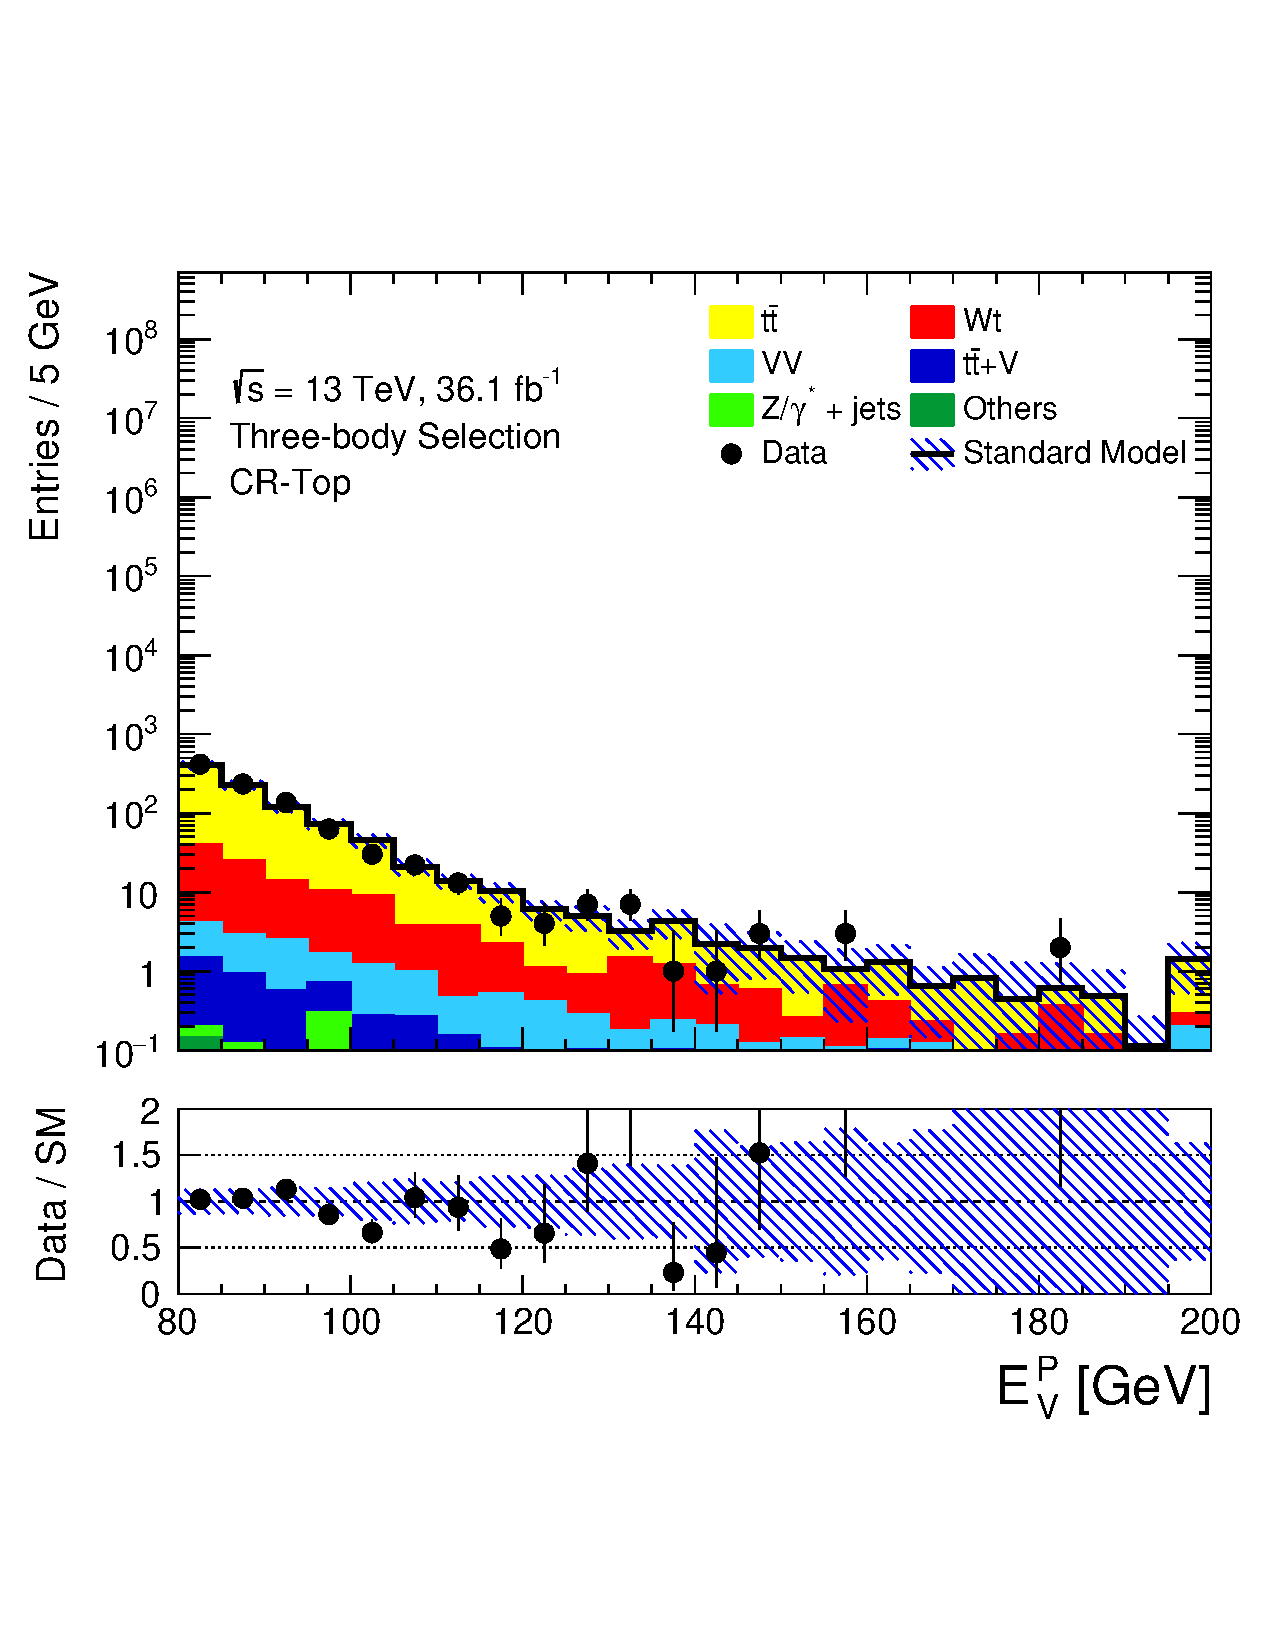
\includegraphics[width=0.48\textwidth]{figures/search_stop2l/bkg_est/crtop/crt_MDR}
        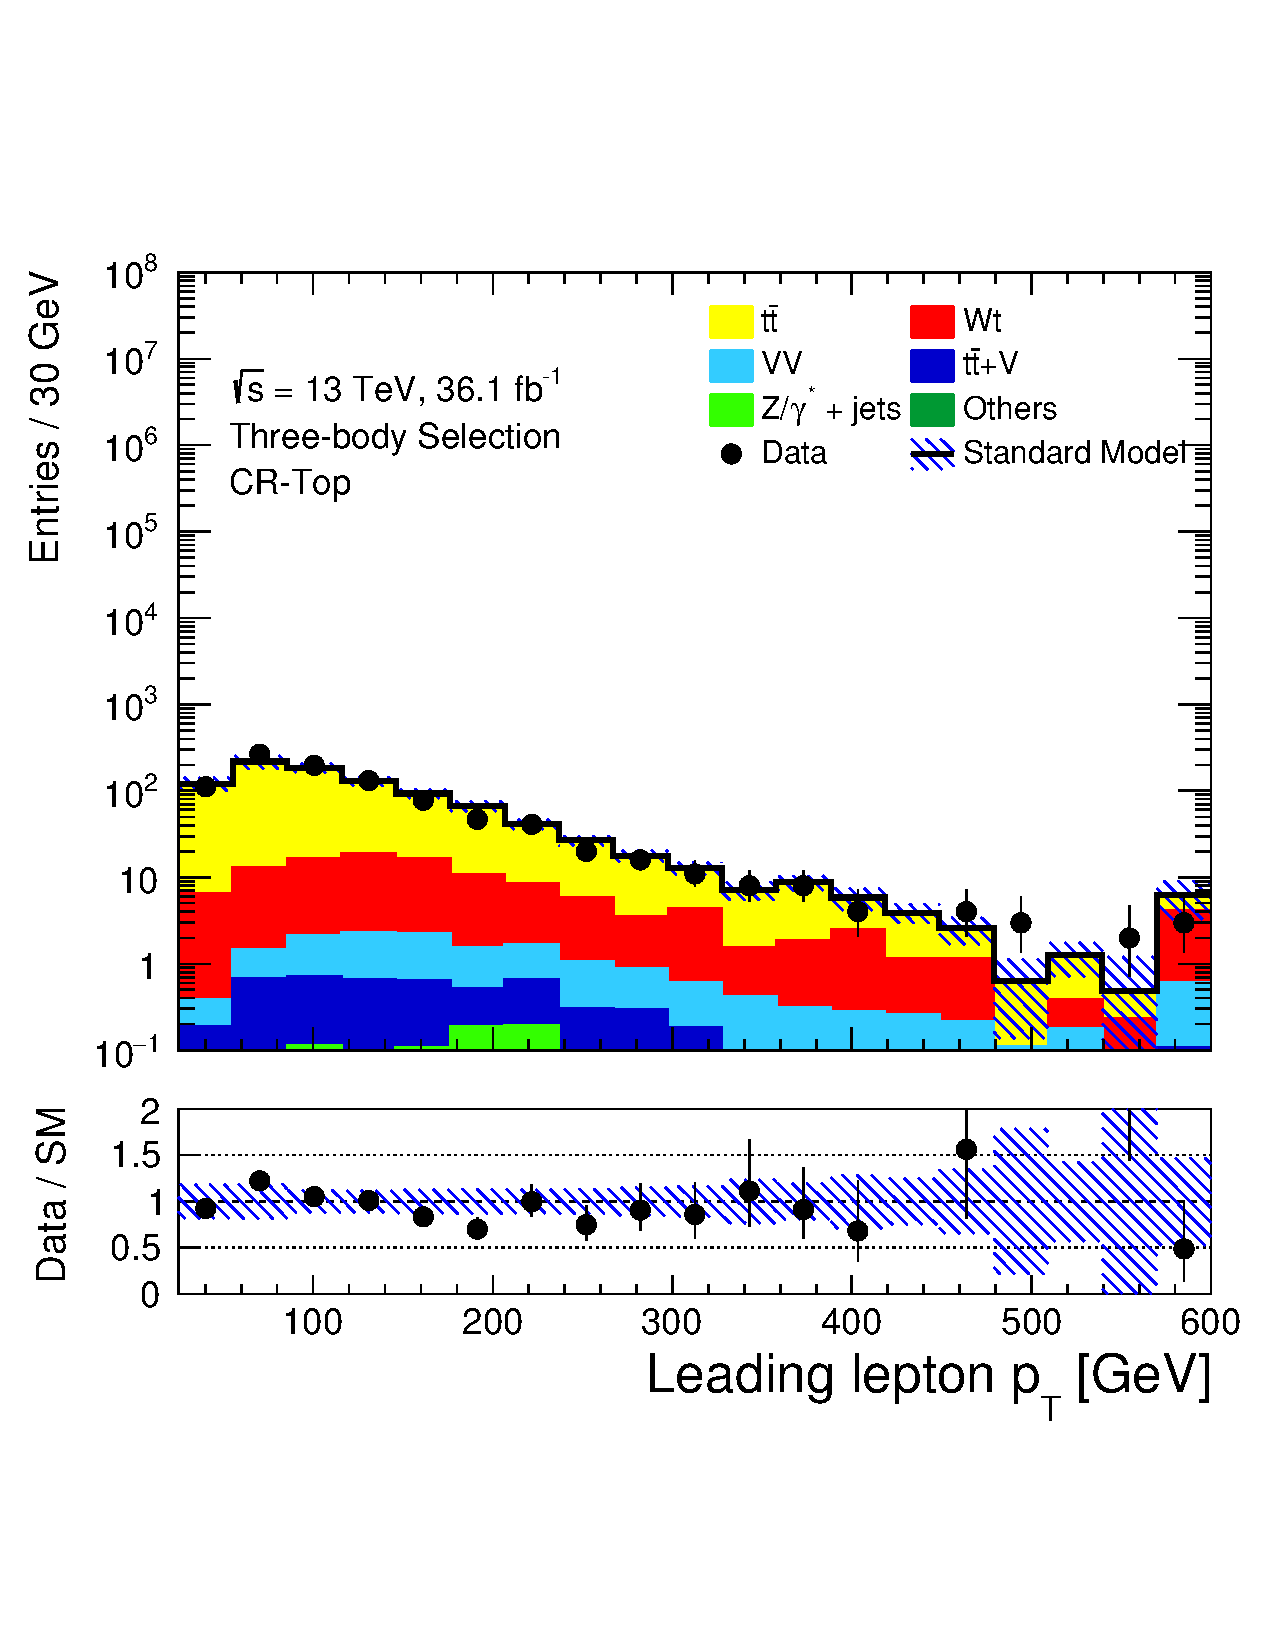
\includegraphics[width=0.48\textwidth]{figures/search_stop2l/bkg_est/crtop/crt_l_pt0}
        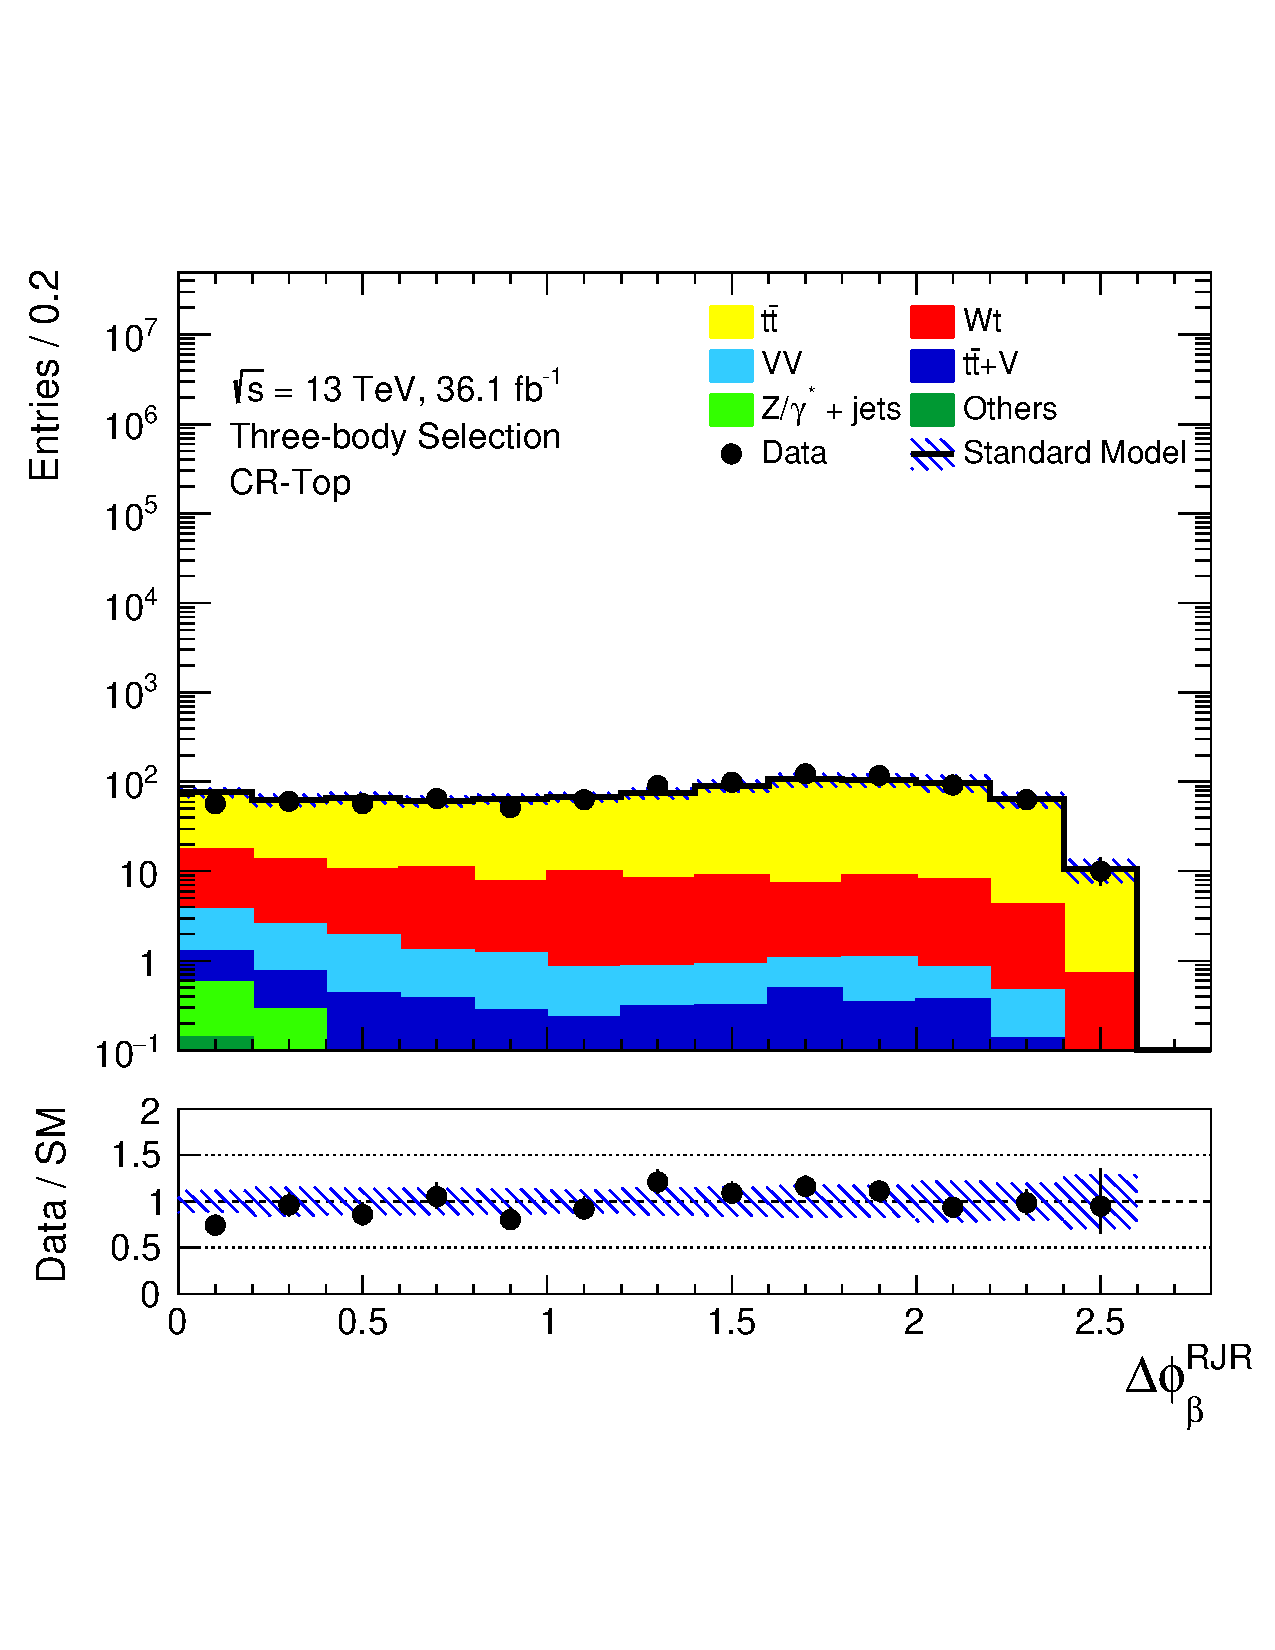
\includegraphics[width=0.48\textwidth]{figures/search_stop2l/bkg_est/crtop/crt_DPB_vSS}
        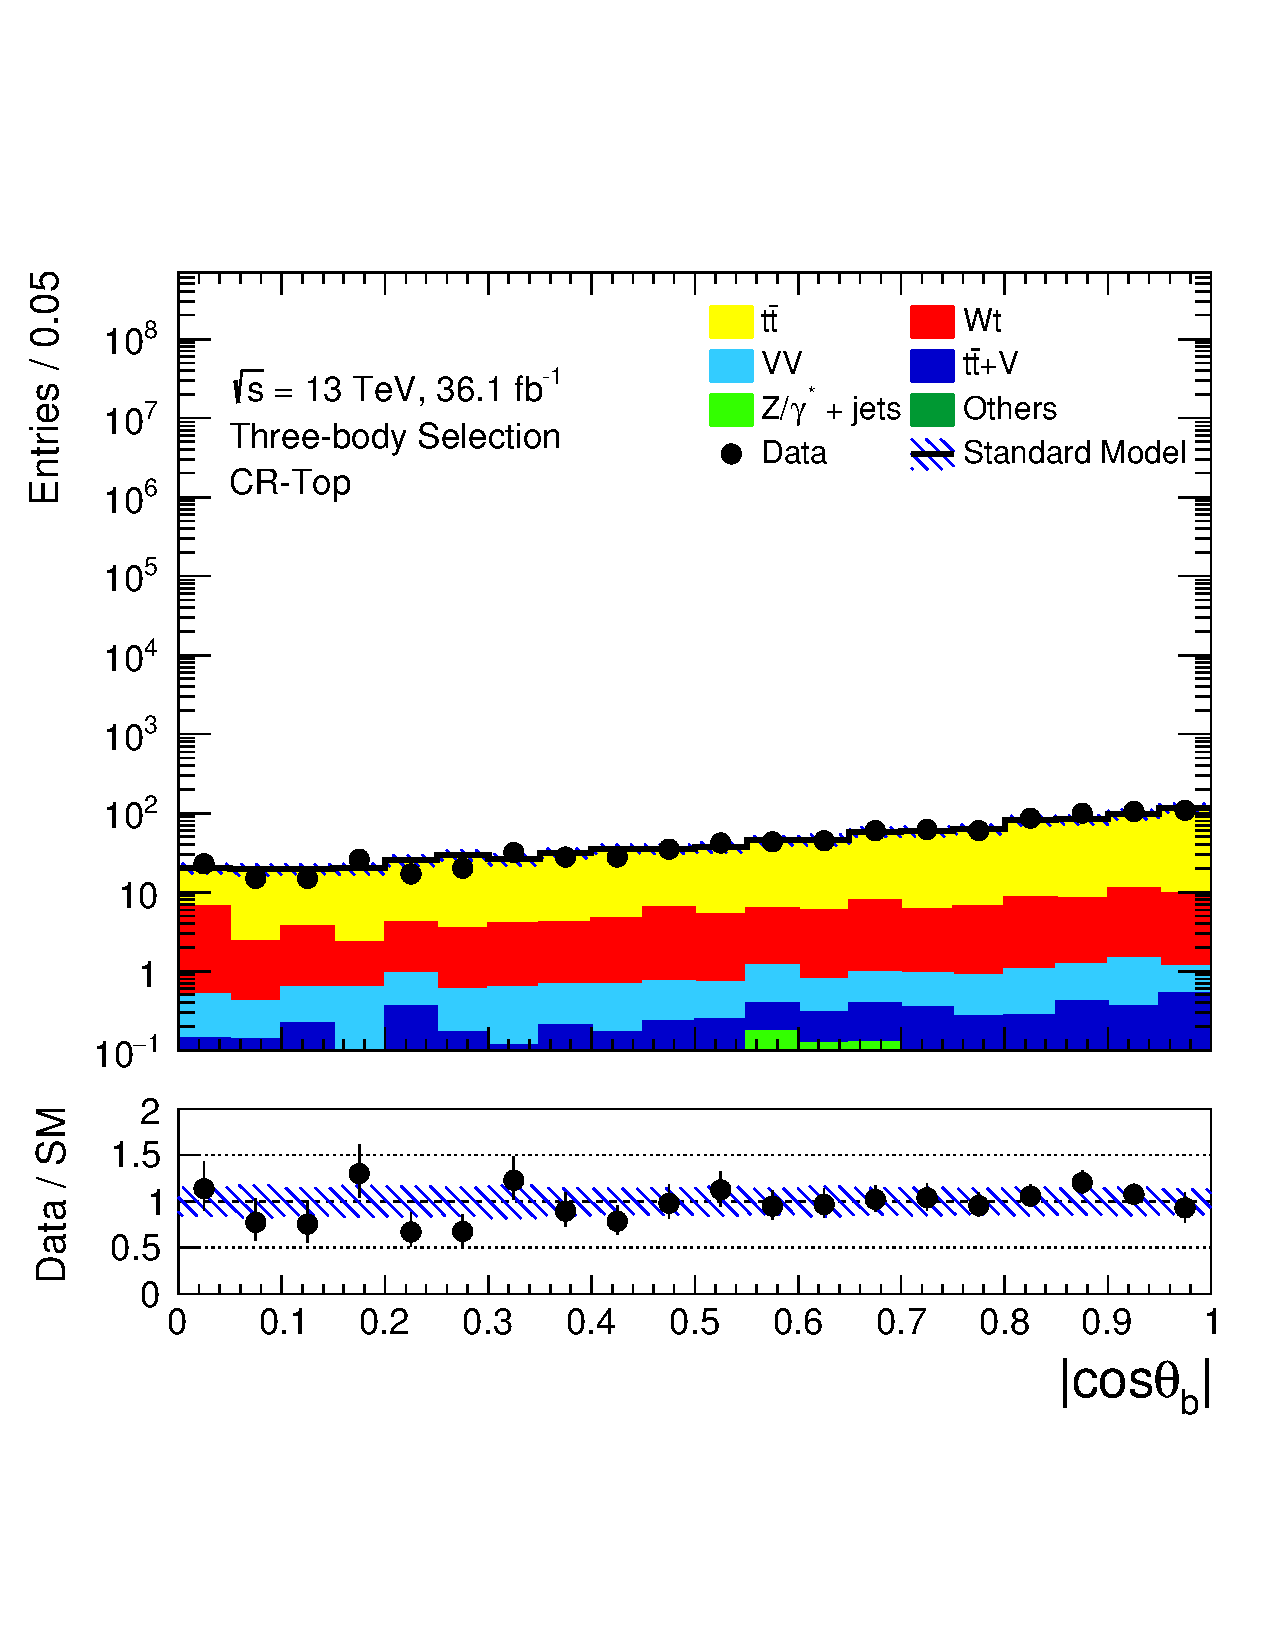
\includegraphics[width=0.48\textwidth]{figures/search_stop2l/bkg_est/crtop/crt_cosThetaB}
        \caption{
            Distributions of \mdr (\textit{\textbf{upper left}}), leading lepton \pT~(\textit{\textbf{upper right}}),
            \dpb (\textit{\textbf{lower left}}), and $|\cosb|$ (\textit{\textbf{lower right}}) in the \ttbar CR,
            CR-Top.
            The error on the SM processes includes statistical and systematic uncertainties.
            The post-fit normalization correction factors for the \ttbar and diboson processes
            have been applied.
        }
        \label{fig:crt_0}
    \end{center}
\end{figure}
\begin{figure}[!htb]
    \begin{center}
        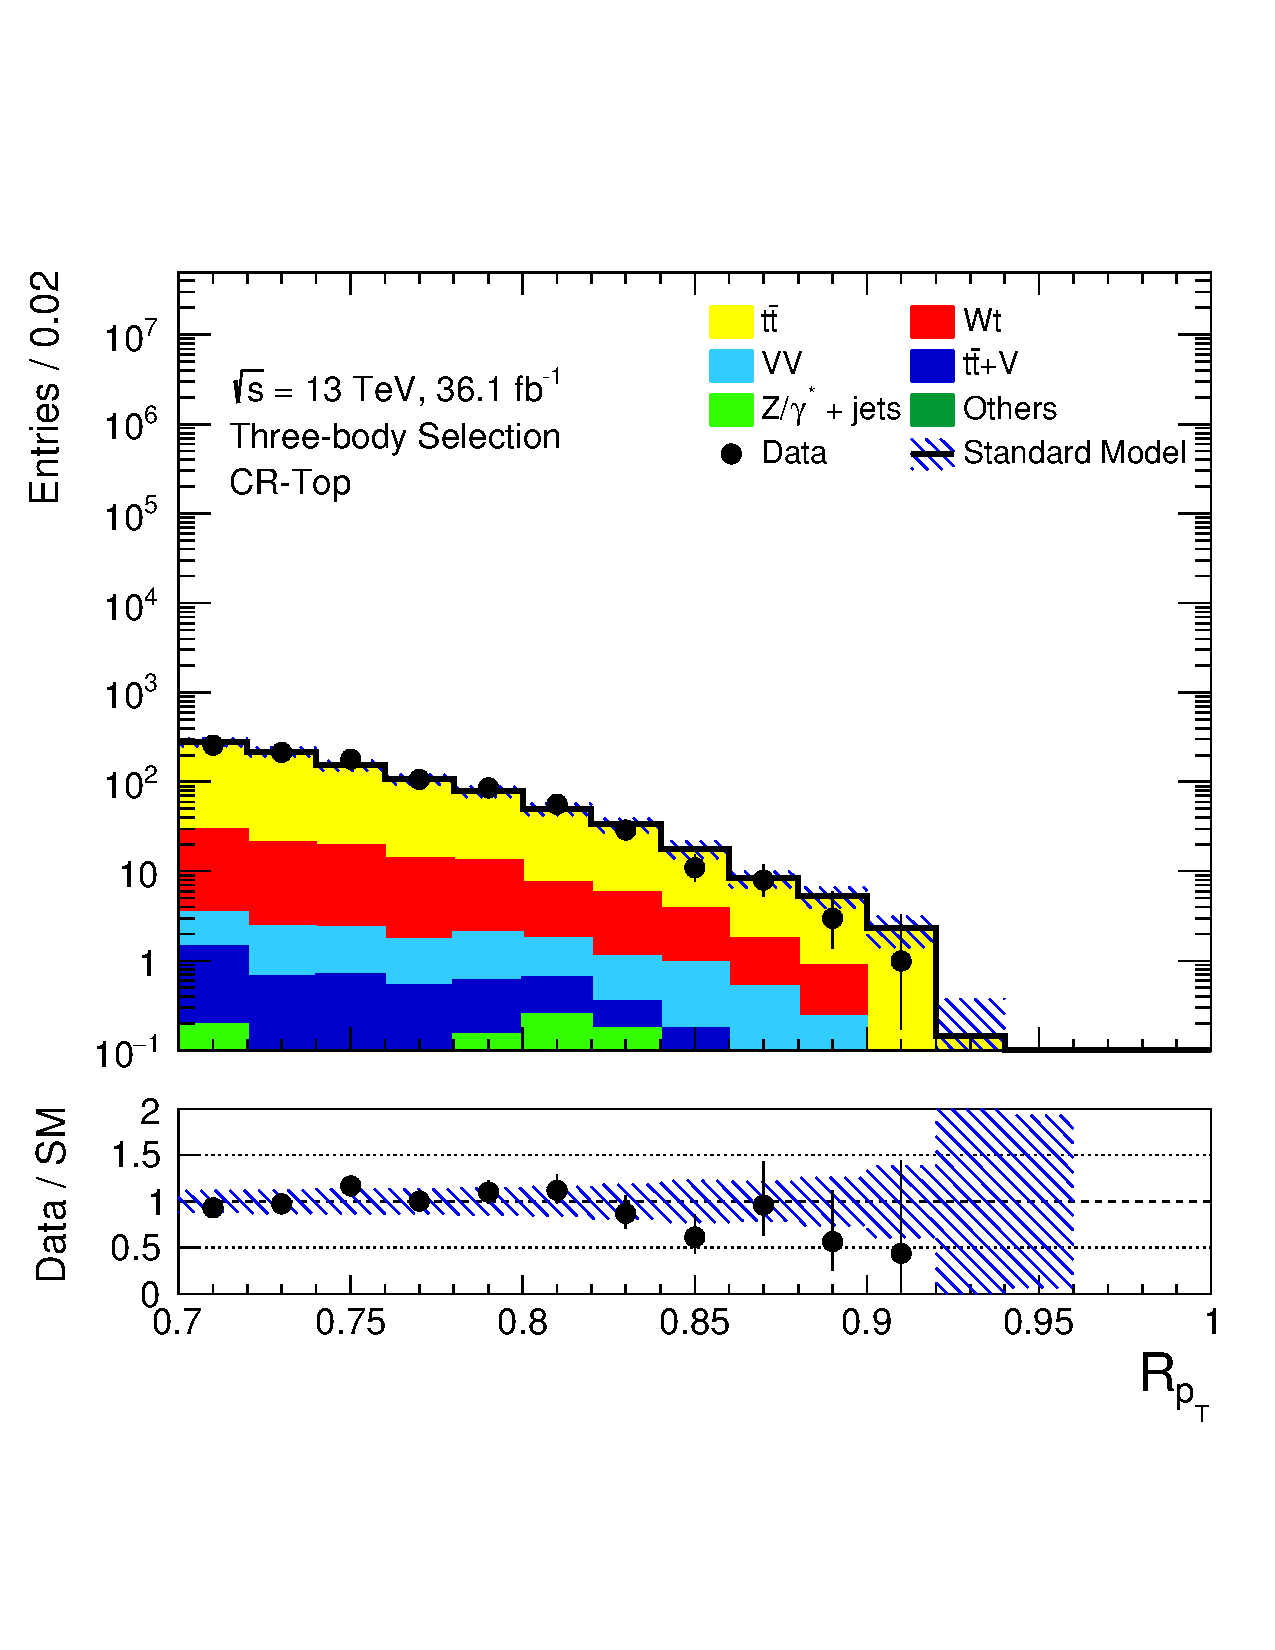
\includegraphics[width=0.48\textwidth]{figures/search_stop2l/bkg_est/crtop/crt_RPT}
        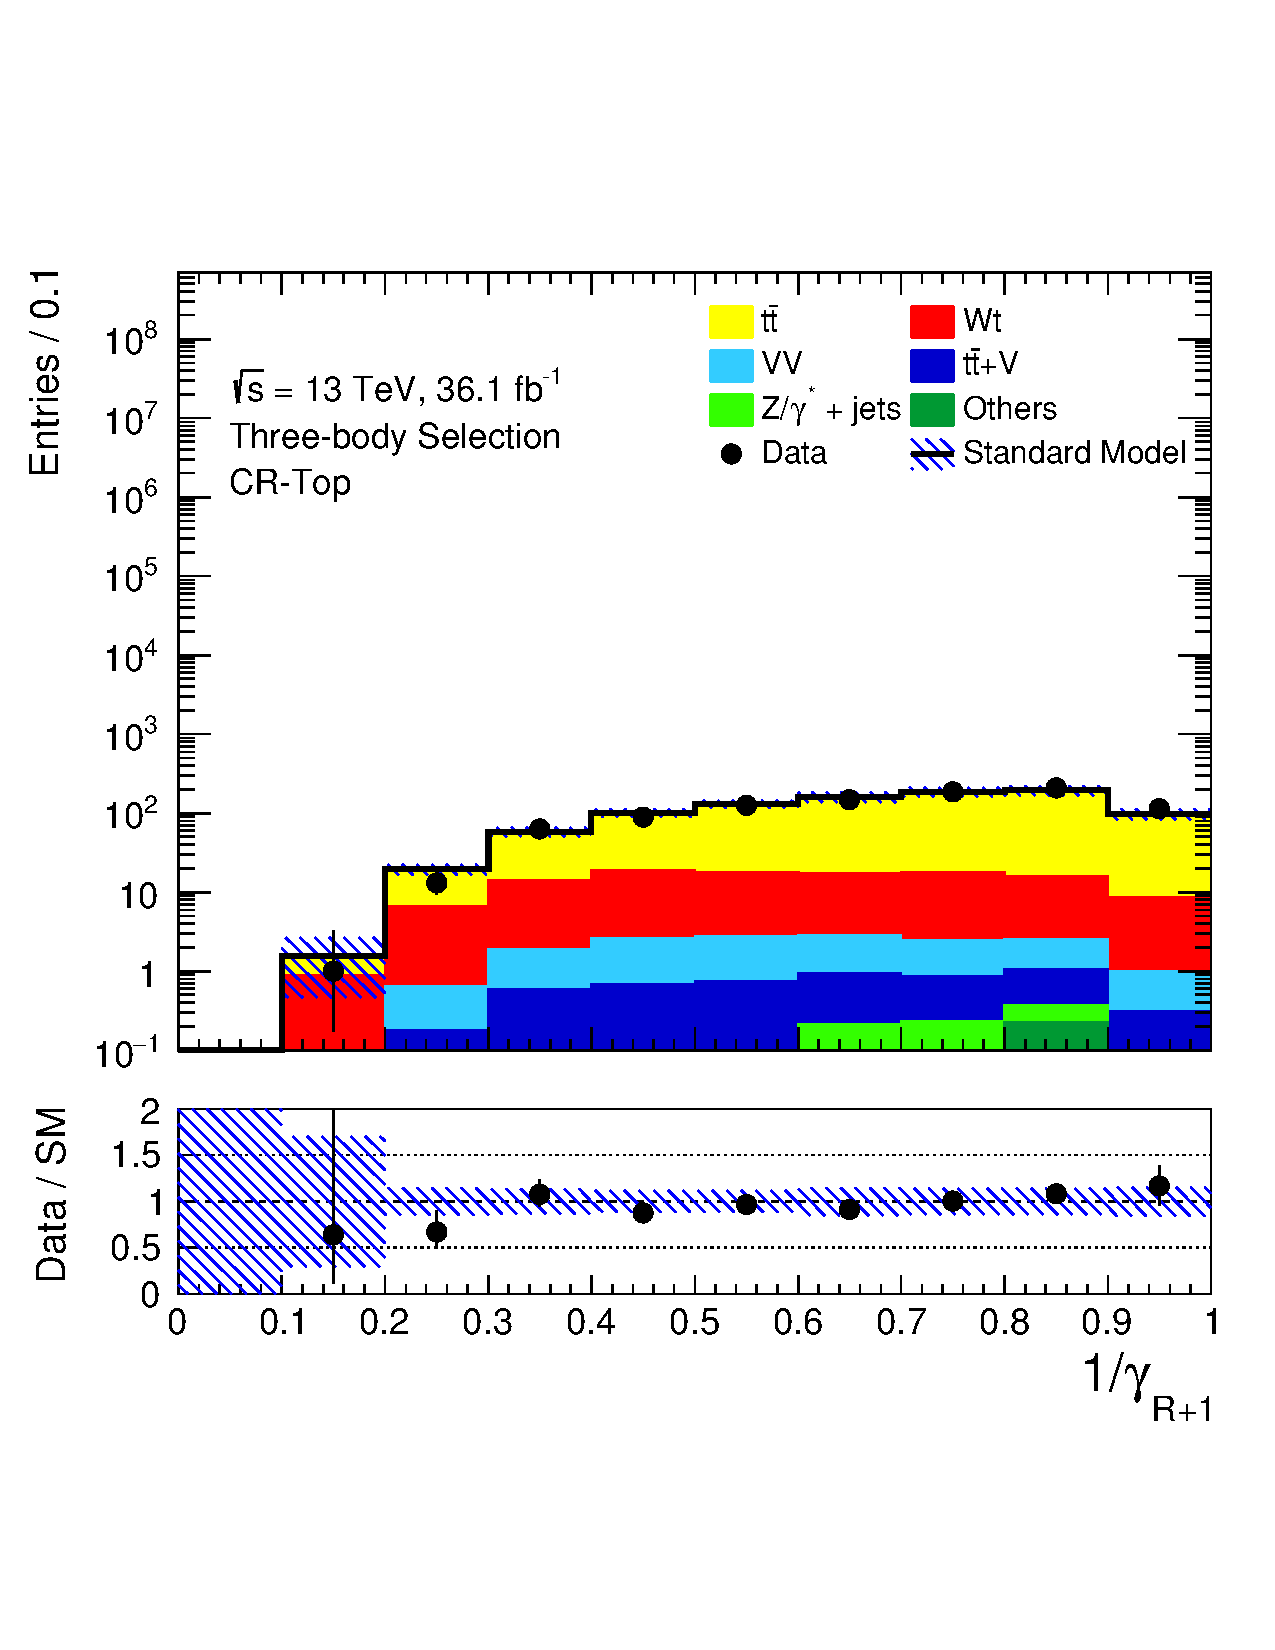
\includegraphics[width=0.48\textwidth]{figures/search_stop2l/bkg_est/crtop/crt_gamInvRp1}
        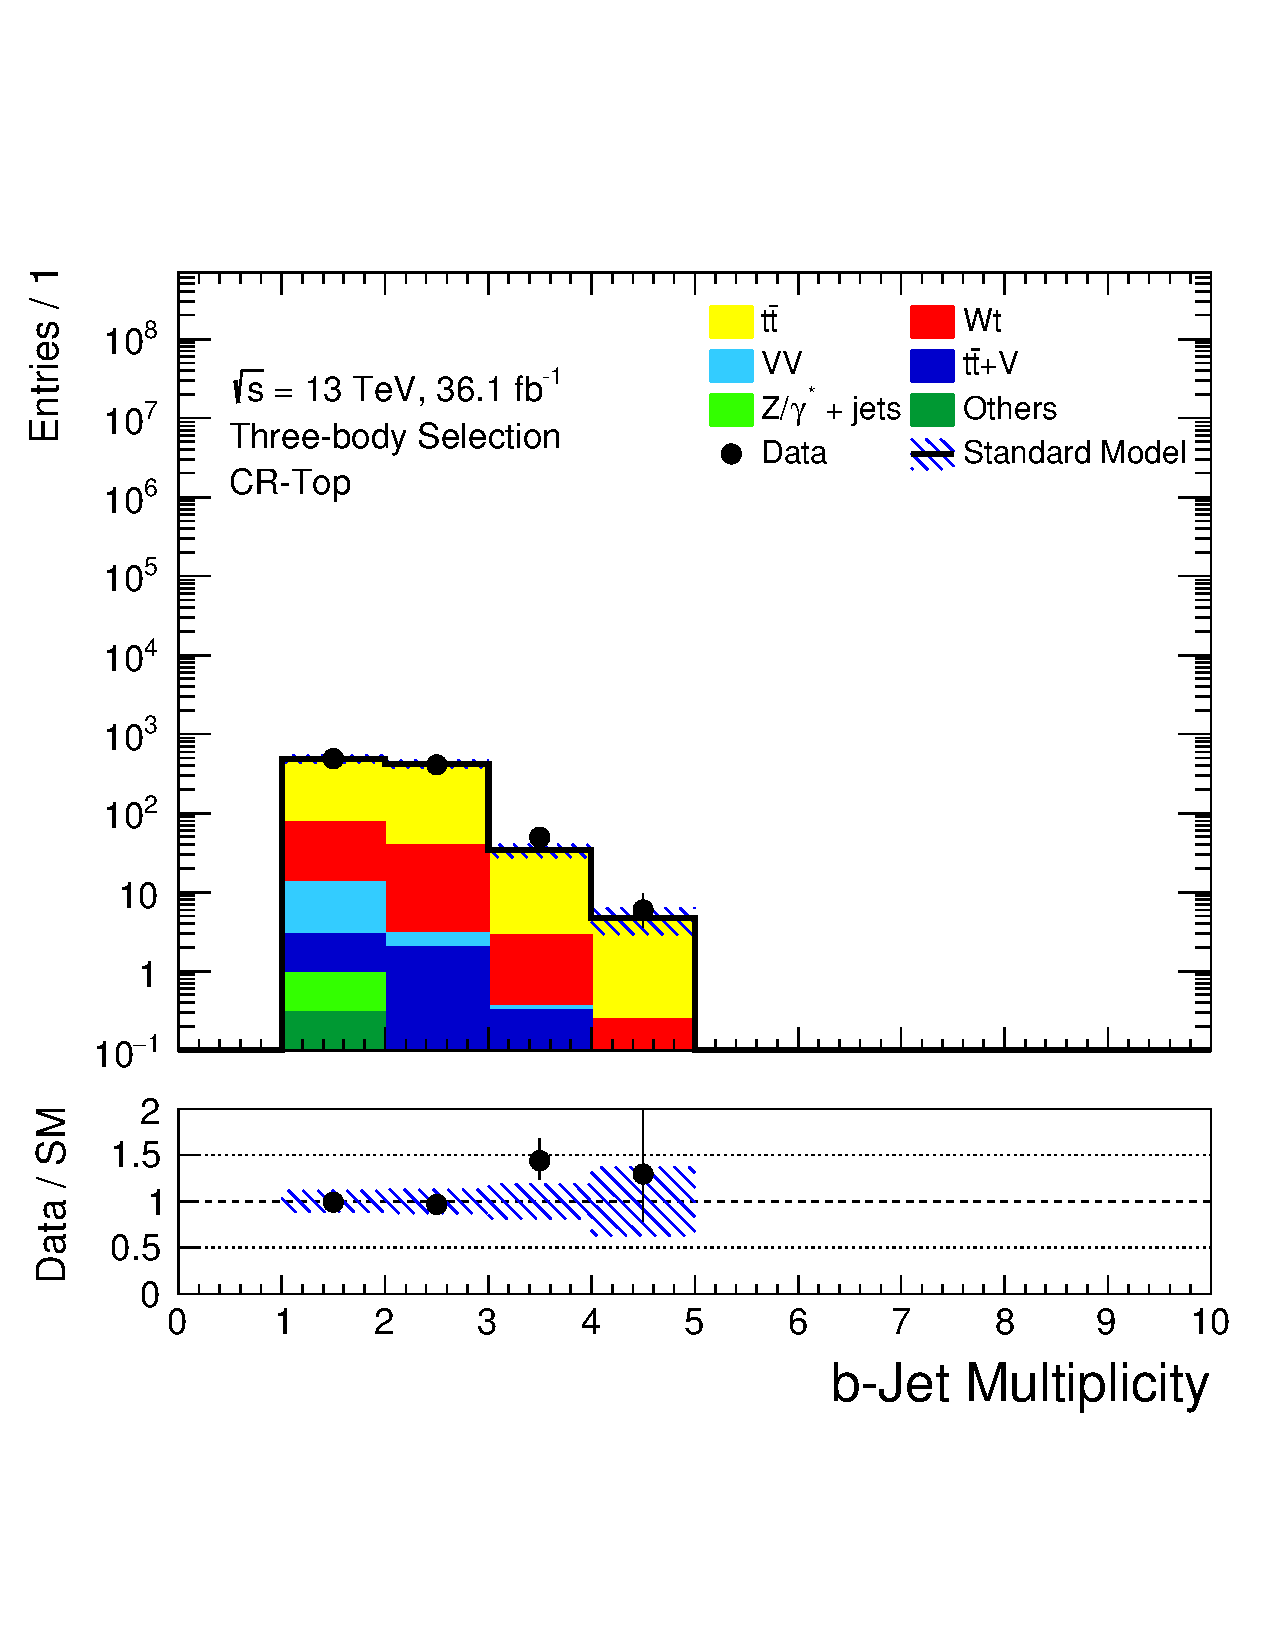
\includegraphics[width=0.48\textwidth]{figures/search_stop2l/bkg_est/crtop/crt_nBJets}
        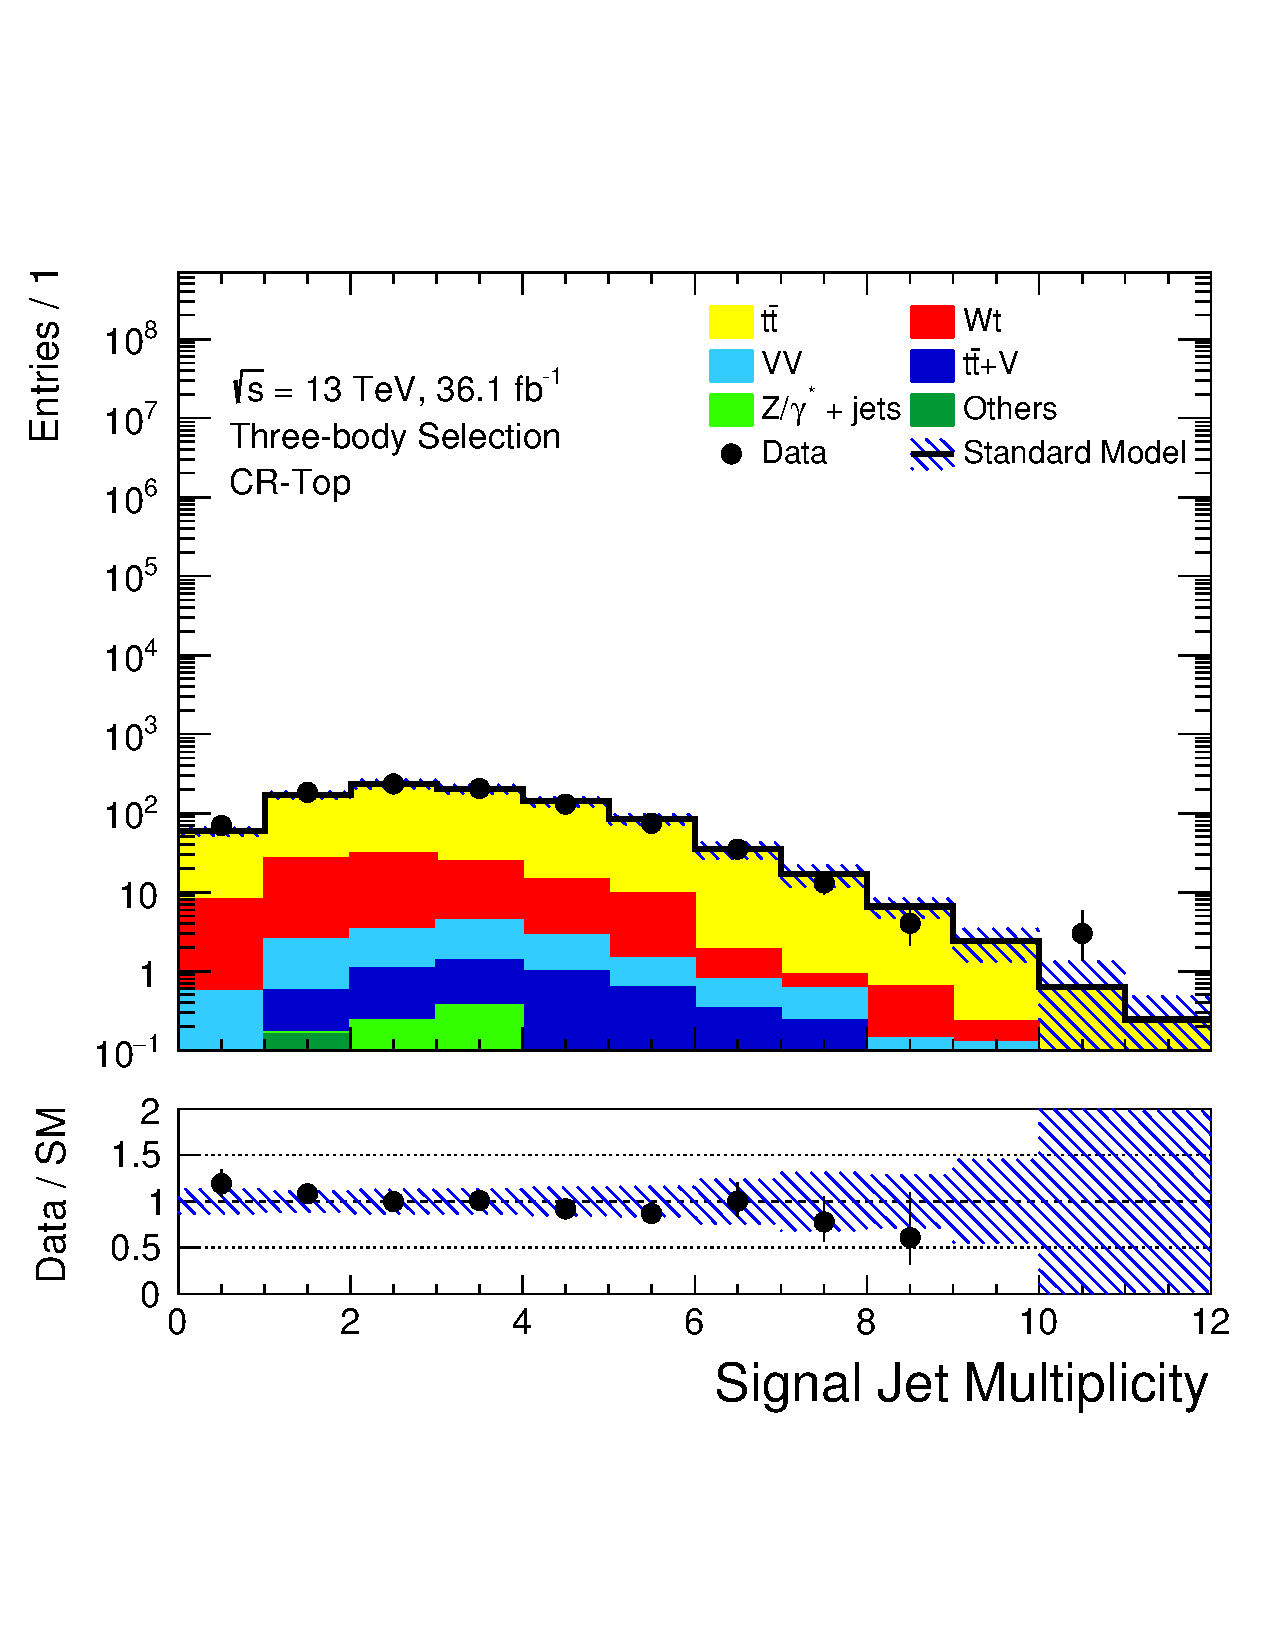
\includegraphics[width=0.48\textwidth]{figures/search_stop2l/bkg_est/crtop/crt_nSJets}
        \caption{
            Distributions of \rpt (\textit{\textbf{upper left}}), leading lepton \gaminv~(\textit{\textbf{upper right}}),
            $b$-tagged jet multiplicity (\textit{\textbf{lower left}}), and non-$b$-tagged jet multiplicity(\textit{\textbf{lower right}}) in the \ttbar CR,
            CR-Top.
            The error on the SM processes includes statistical and systematic uncertainties.
            The post-fit normalization correction factors for the \ttbar and diboson processes
            have been applied.
        }
        \label{fig:crt_1}
    \end{center}
\end{figure}



%%%%%%%%%%%%%%%%%%%%%%%%%%%%%%%%%%%%%%%%%%%%%%%%%%%%%%%%%%%%%%%%%%%%%%%%%%%%%%%%%%%%%%%%%%%%
%%%%%%%%%%%%%%%%%%%%%%%%%%%%%%%%%%%%%%%%%%%%%%%%%%%%%%%%%%%%%%%%%%%%%%%%%%%%%%%%%%%%%%%%%%%%
%%%%%%%%%%%%%%%%%%%%%%%%%%%%%%%%%%%%%%%%%%%%%%%%%%%%%%%%%%%%%%%%%%%%%%%%%%%%%%%%%%%%%%%%%%%%
%
% VV BKG
%
%%%%%%%%%%%%%%%%%%%%%%%%%%%%%%%%%%%%%%%%%%%%%%%%%%%%%%%%%%%%%%%%%%%%%%%%%%%%%%%%%%%%%%%%%%%%
%%%%%%%%%%%%%%%%%%%%%%%%%%%%%%%%%%%%%%%%%%%%%%%%%%%%%%%%%%%%%%%%%%%%%%%%%%%%%%%%%%%%%%%%%%%%
%%%%%%%%%%%%%%%%%%%%%%%%%%%%%%%%%%%%%%%%%%%%%%%%%%%%%%%%%%%%%%%%%%%%%%%%%%%%%%%%%%%%%%%%%%%%

\subsection{Diboson Production}
\label{sec:stop_vv_estimate}

The SM diboson processes are composed of $WW$, $ZW+WZ$, and $ZZ$ production.
The dominant process for the \bWN SRs is $WW$, as discussed in the text.
In order to constrain the $WW$ component, in addition to those components with a $Z$ boson,
the diboson CRs are split into two, one targeting the different-flavor enriched component
of the diboson background (predominantly $WW$) and one in which the same-flavor component ($ZW+WZ$ and $ZZ$)
is enriched.

The same-flavor and different-flavor diboson CRs (VRs), CR-VV-SF and CR-VV-DF (VR-VV-SF and VR-VV-DF), respectively,
are defined in Table~\ref{tab:stop_vv_crvr}.
All of the regions apply a $b$-tagged jet veto.
Although there are SRs that are inclusive of $b$-tagged jets (SRt-SF and SRt-DF), the diboson background
is negligible in them and so the normalisation correction factors derived in the diboson CRs
can be extrapolated with confidence into the SRs with a $b$-tagged jet veto (SRw-SF and SRw-DF).
There is no difference between the same-flavor and different-flavor CRs, apart from the dilepton flavor
requirements and $Z$-veto.
The diboson VRs have the same, or inclusive, \rpt and \gaminv  selections as the CRs but have orthogonal
\mdr requirements that move them closer the SR selections.

Distributions of several key observables in CR-VV-SF (CR-VV-DF) are shown in Figures~\ref{fig:crvvSF_0}-\ref{fig:crvvSF_1}
(Figures~\ref{fig:crvvDF_0}-\ref{fig:crvvDF_1}).

\begin{table}[!htb]
    \begin{center}
        \begin{scriptsize}
        \caption{
            Definitions of the CR and VR for the diboson~background processes for the
            \bWN search.
        }
        \label{tab:stop_vv_crvr}
        \begin{tabular}{l | c c c c}
            \hline
            \hline
                & \multicolumn{4}{c}{\textbf{Regions}} \\
            \hline
            \textbf{Variable} & \textbf{CR-VV-DF} & \textbf{CR-VV-SF} & \textbf{VR-VV-DF} & \textbf{VR-VV-SF} \\
            \hline
            Dilepton Flavor & DF & SF & DF & SF \\
            $m_{\ell\ell}$ [GeV]    & no req. & $|m_{\ell\ell} - 91.2| > 10$ & no req. & $|m_{\ell\ell} - 91.2| > 10$ \\
            Lead lepton \pT~[GeV] & $>25$ & $>25$ & $>25$ & $>25$ \\
            Sub-lead lepton \pT~[GeV] & $>20$ & $>20$ & $>20$ & $>20$ \\
            $b$-tagged jet multiplicity & Exactly 0 & Exactly 0 & Exactly 0 & Exactly 0 \\
            \mdr [GeV] & $>50$ & $>70$ & $\in(50,95)$ & $\in(60,95)$ \\
            \rpt & $<0.5$ & $<0.5$ & $<0.7$ & $<0.4$ \\
            \gaminv &  $>0.7$ & $>0.7$ & $>0.7$ & $>0.7$ \\
            $(\cosb, \dpb)$ & \multicolumn{2}{c}{\small{$\dpb < 0.9 \times | \cosb | + 1.6$}} & \multicolumn{2}{c}{\small{$\dpb> 0.9 \times | \cosb | + 1.6$}} \\
            \hline
            \hline
        \end{tabular}
        \end{scriptsize}
    \end{center}
\end{table}

\begin{figure}[!htb]
    \begin{center}
        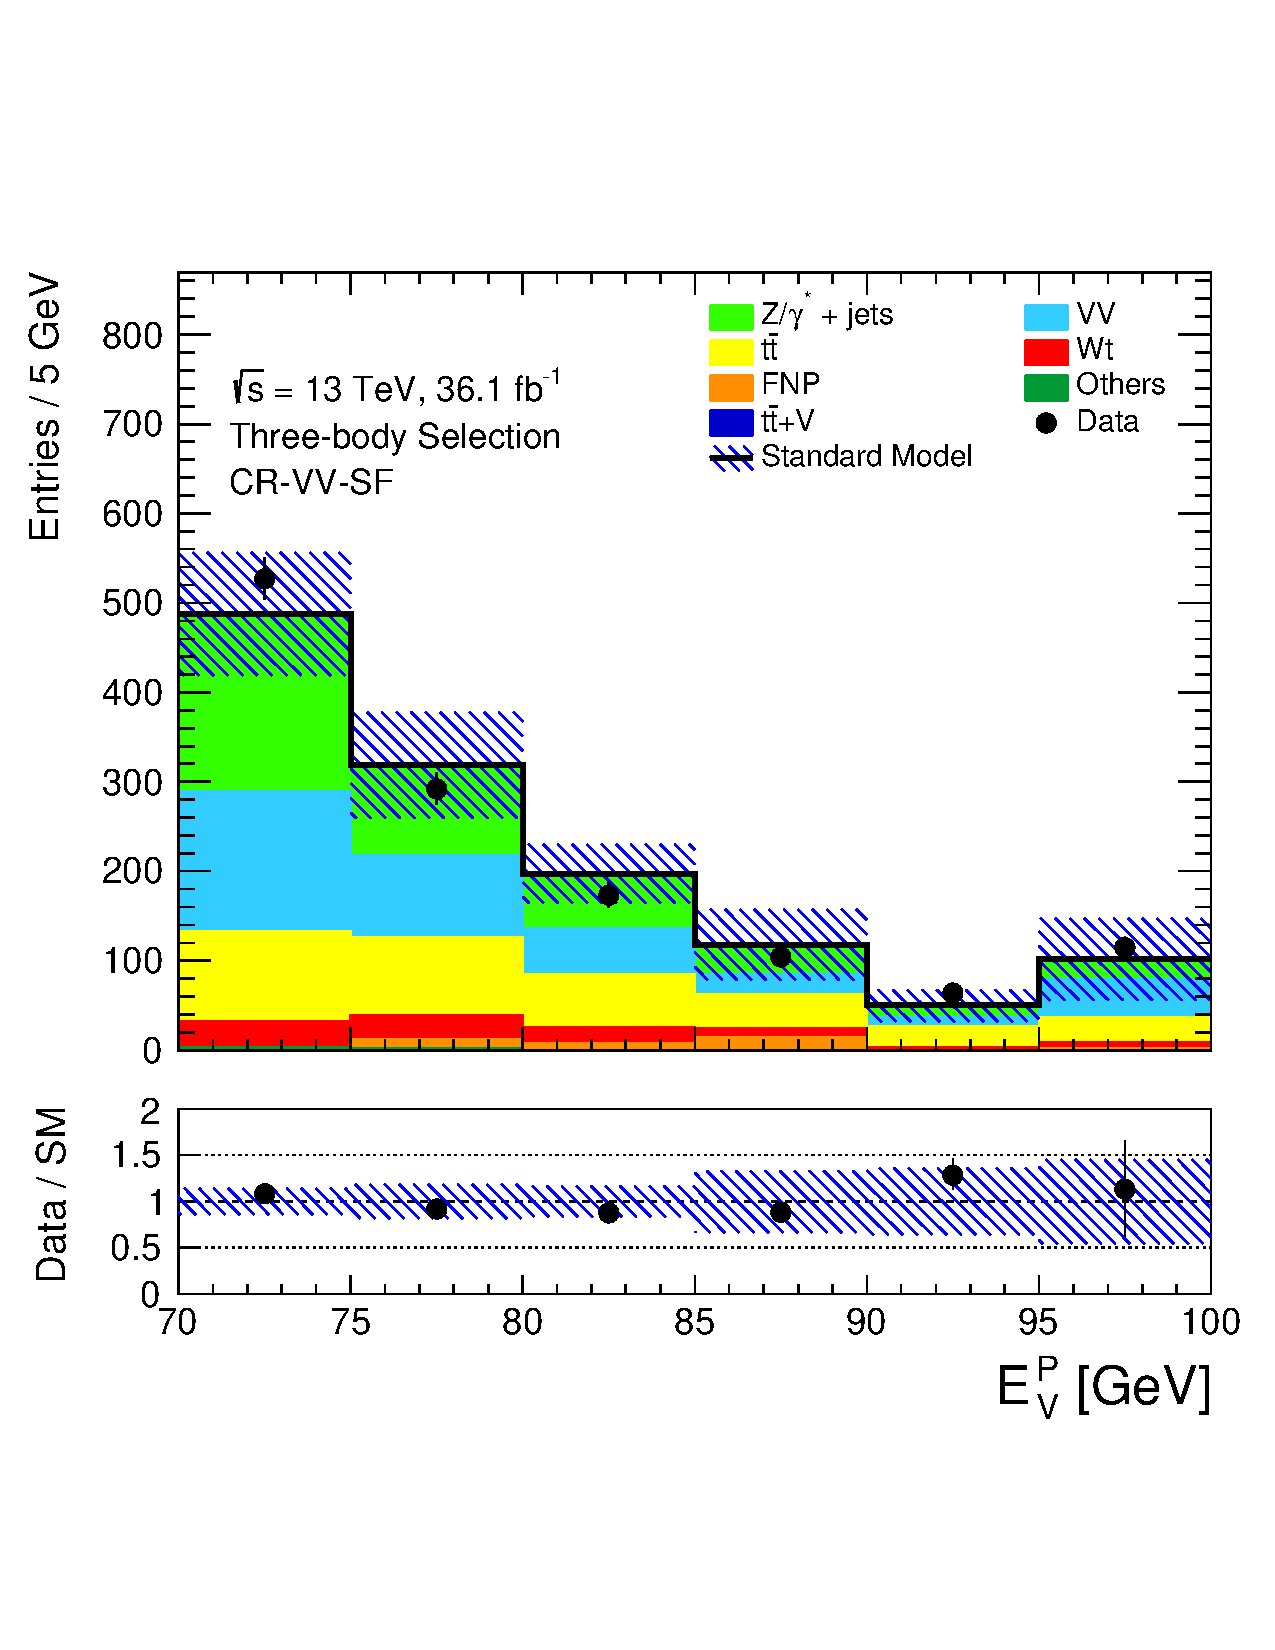
\includegraphics[width=0.48\textwidth]{figures/search_stop2l/bkg_est/crvsf/crvSF_MDR}
        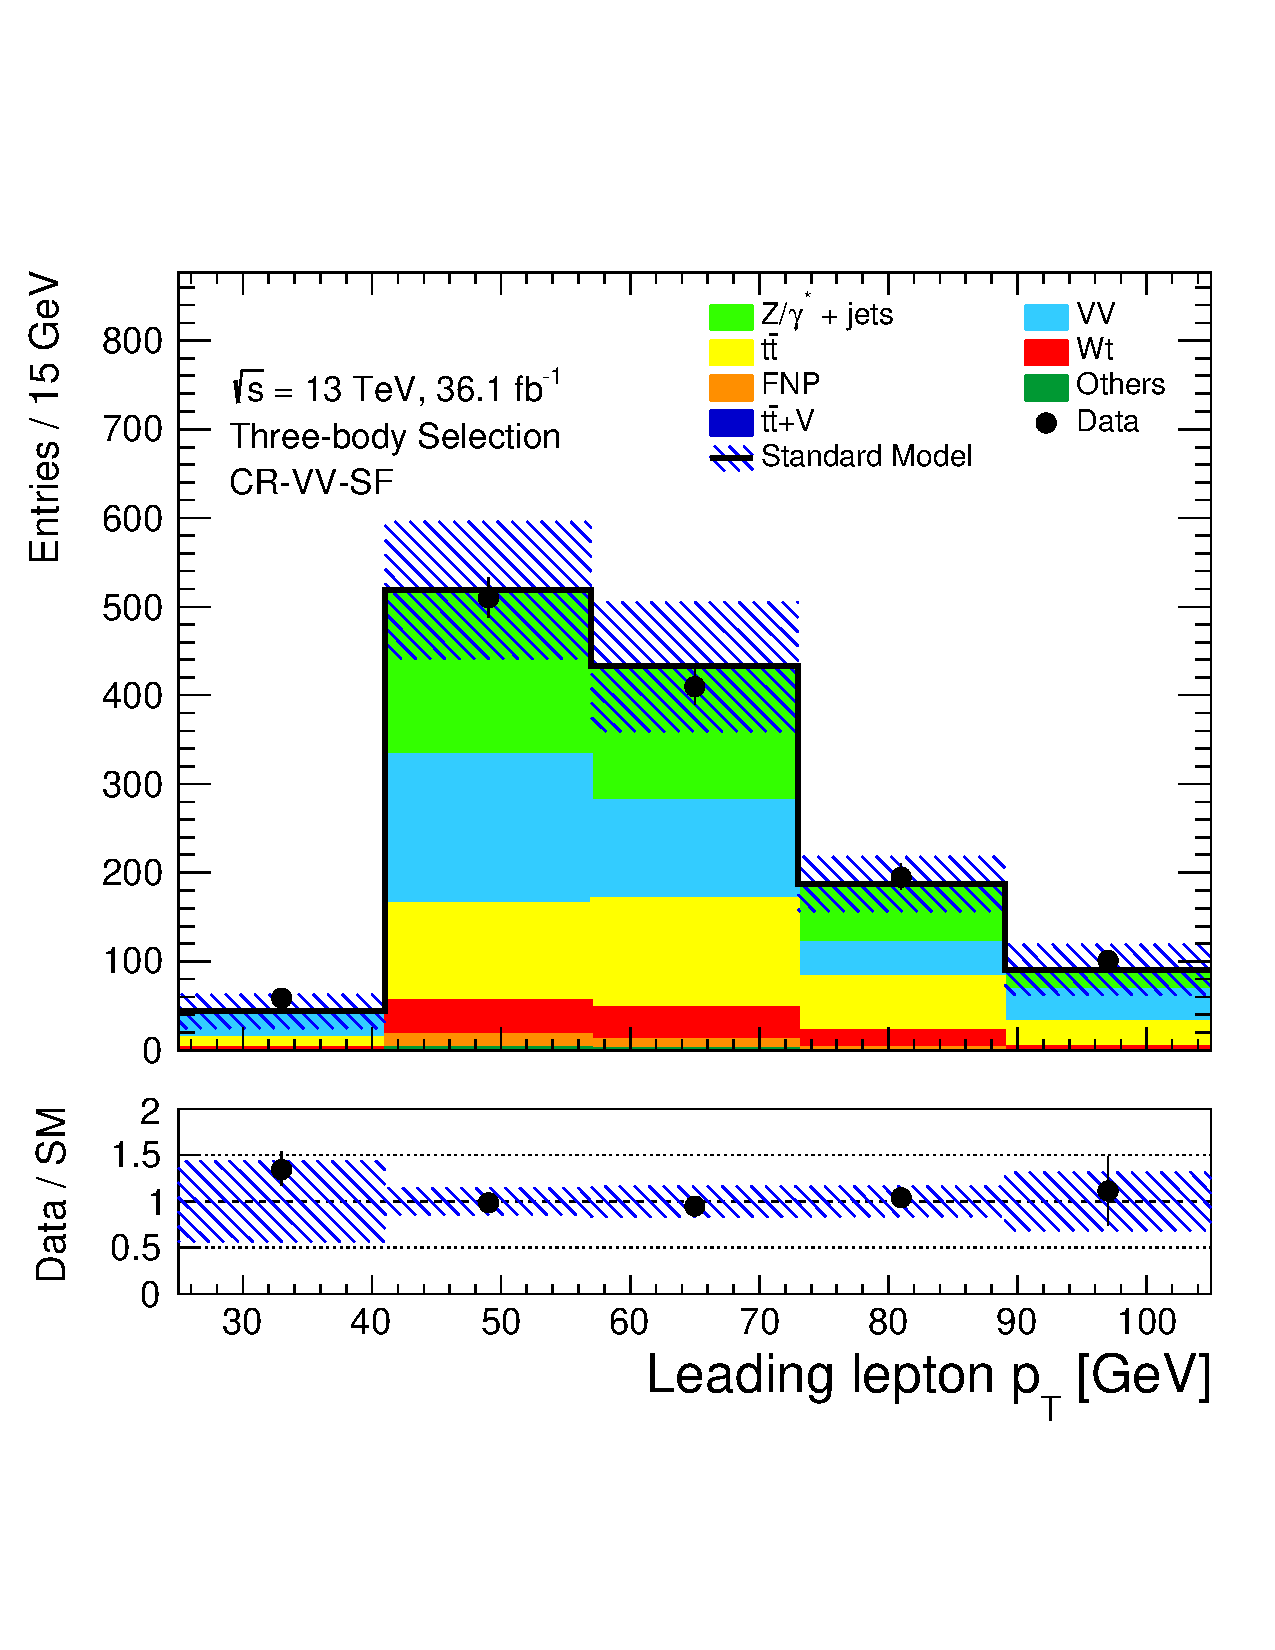
\includegraphics[width=0.48\textwidth]{figures/search_stop2l/bkg_est/crvsf/crvSF_l_pt0}
        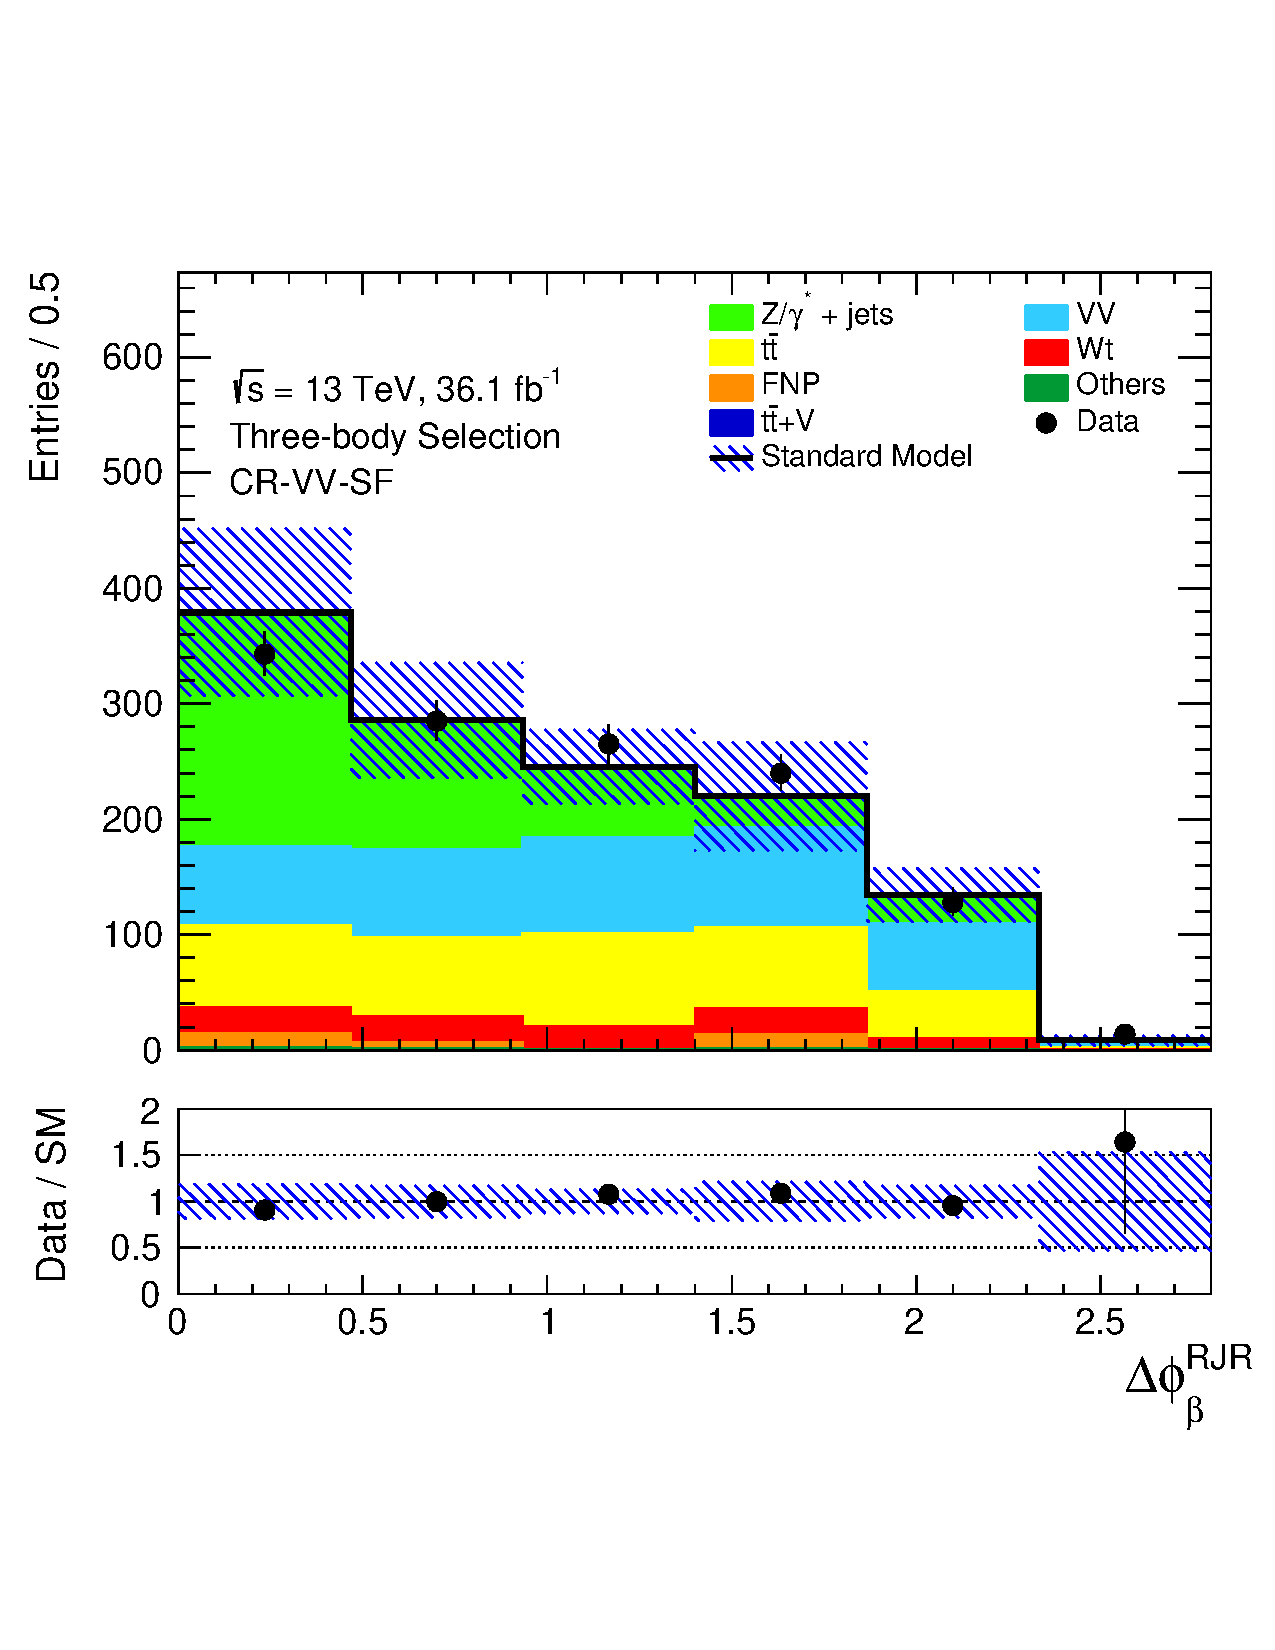
\includegraphics[width=0.48\textwidth]{figures/search_stop2l/bkg_est/crvsf/crvSF_DPB_vSS}
        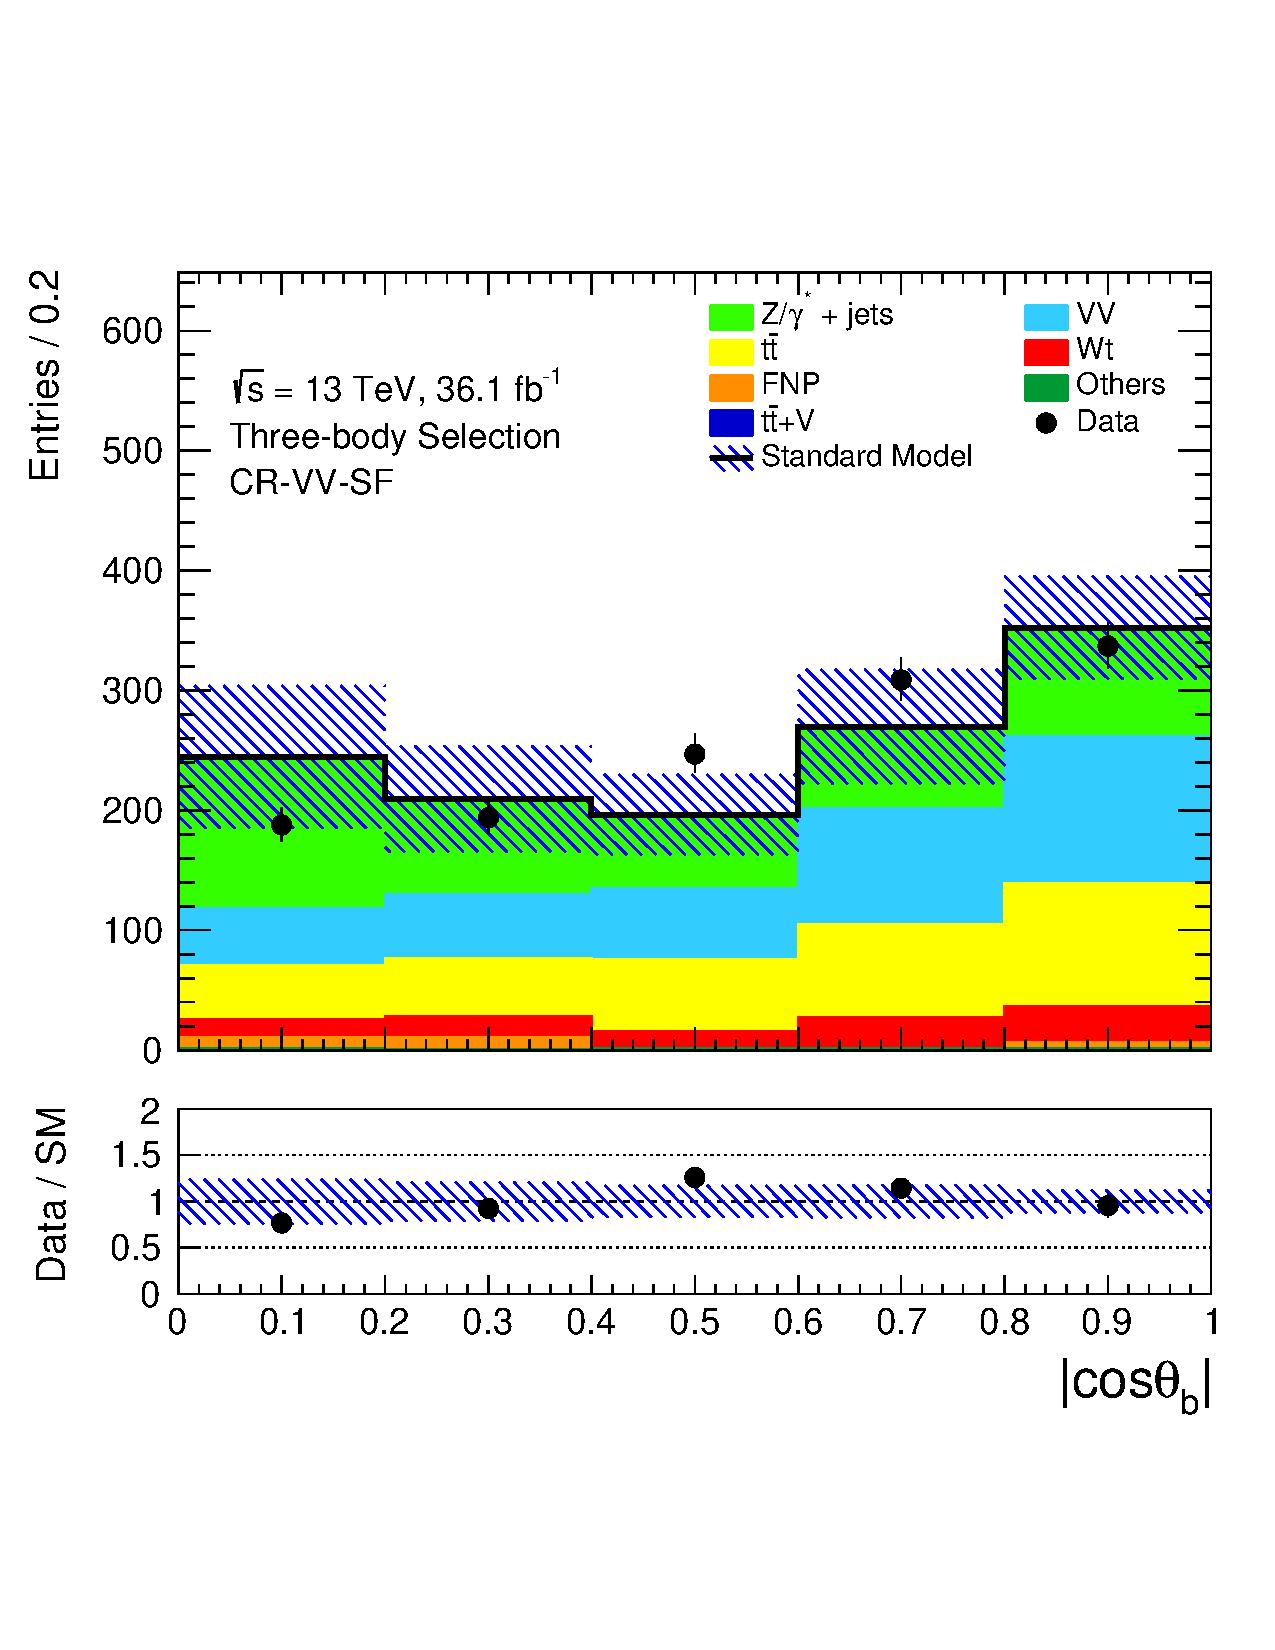
\includegraphics[width=0.48\textwidth]{figures/search_stop2l/bkg_est/crvsf/crvSF_cosThetaB}
        \caption{
            Distributions of \mdr (\textit{\textbf{upper left}}), leading lepton \pT~(\textit{\textbf{upper right}}),
            \dpb (\textit{\textbf{lower left}}), and $|\cosb|$ (\textit{\textbf{lower right}}) in the same-flavor diboson CR,
            CR-VV-SF.
            The error on the SM processes includes statistical and systematic uncertainties.
            The post-fit normalization correction factors for the \ttbar and diboson processes
            have been applied.
        }
        \label{fig:crvvSF_0}
    \end{center}
\end{figure}
\begin{figure}[!htb]
    \begin{center}
        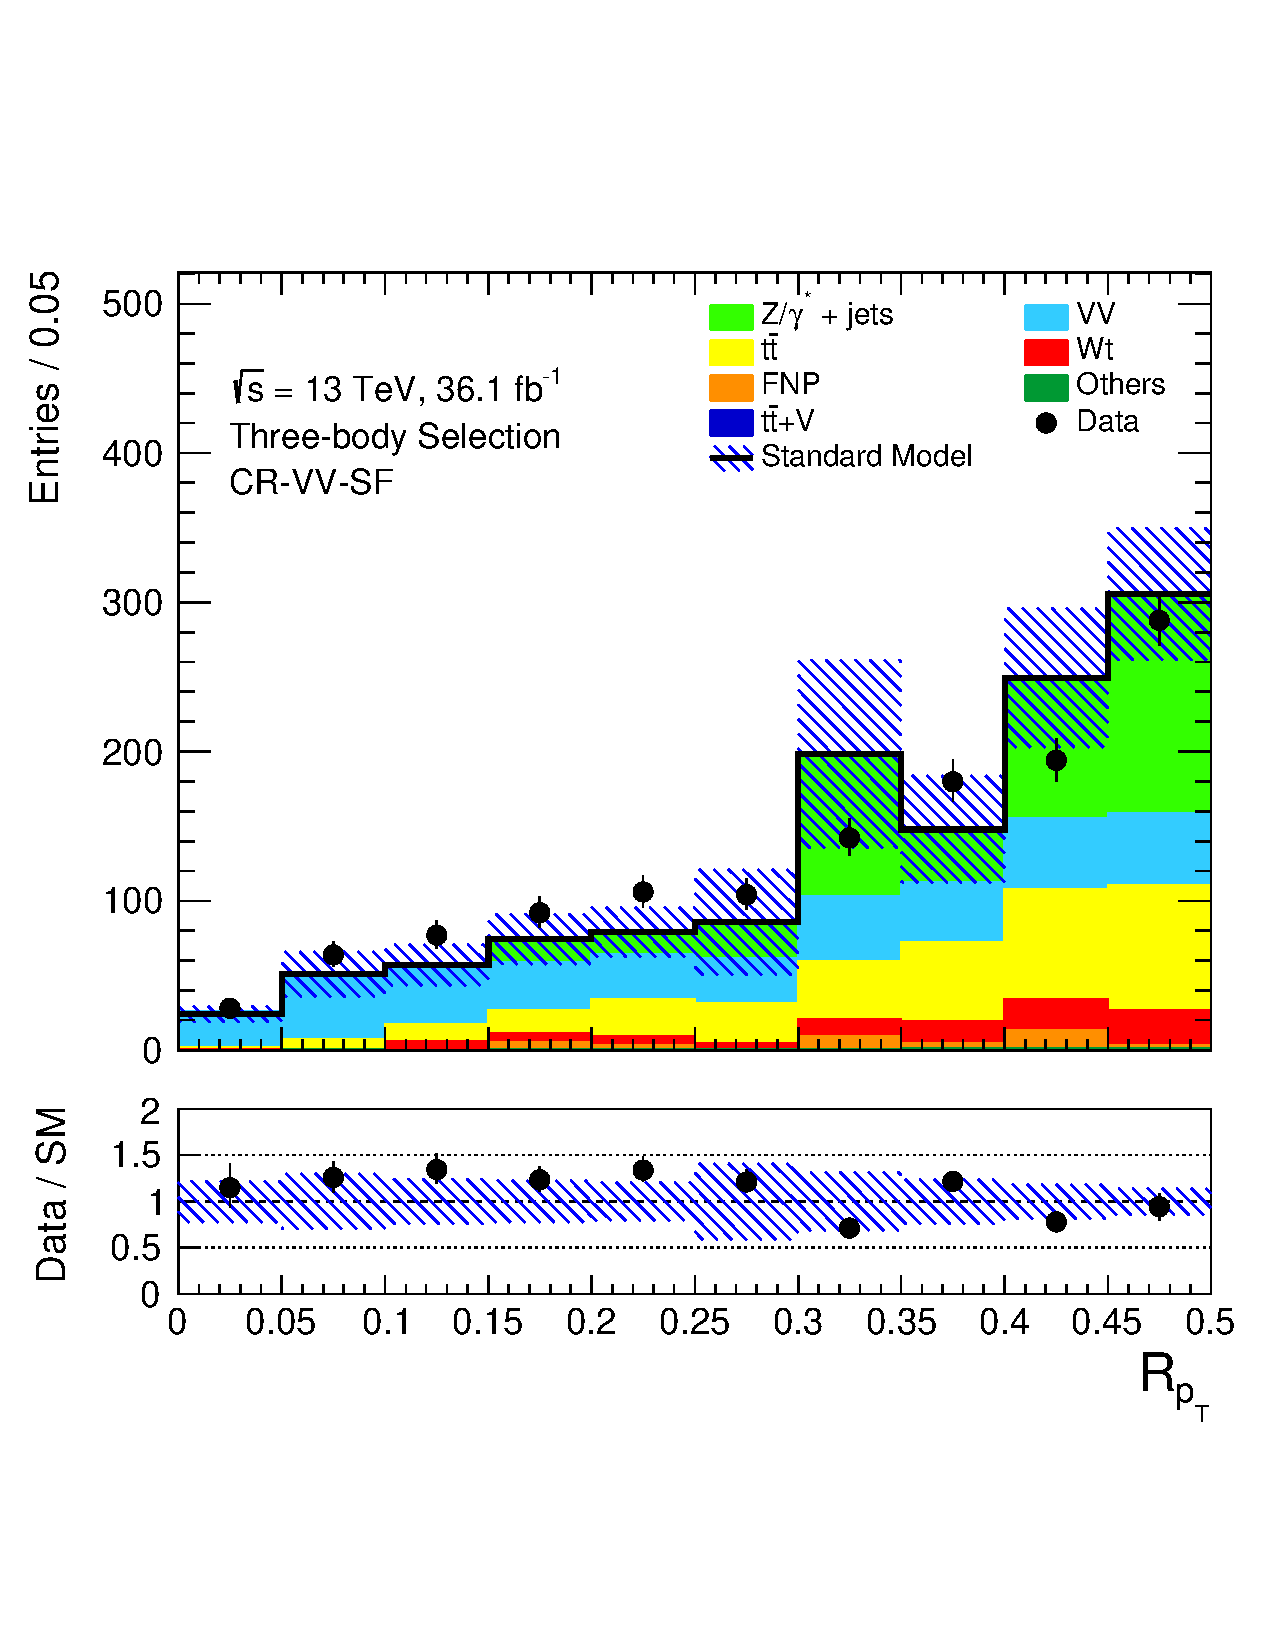
\includegraphics[width=0.48\textwidth]{figures/search_stop2l/bkg_est/crvsf/crvSF_RPT}
        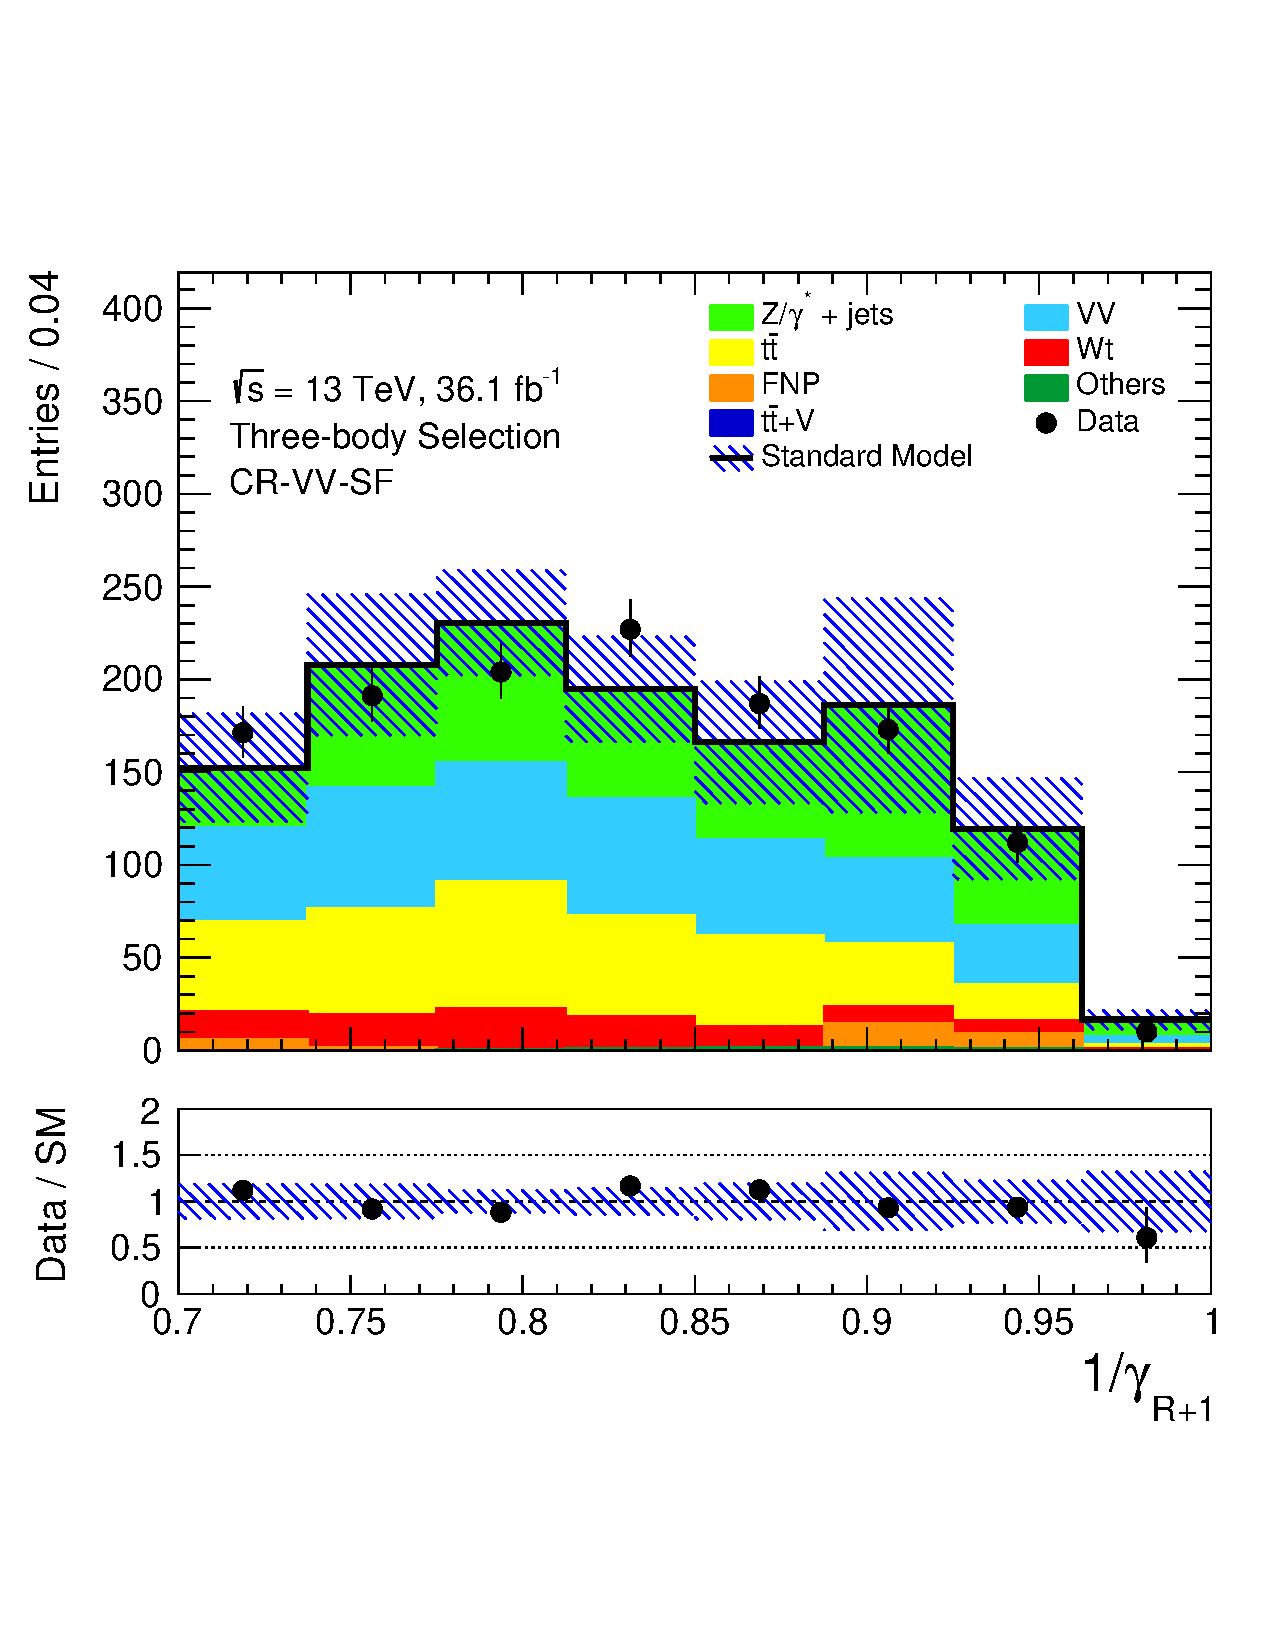
\includegraphics[width=0.48\textwidth]{figures/search_stop2l/bkg_est/crvsf/crvSF_gamInvRp1}
        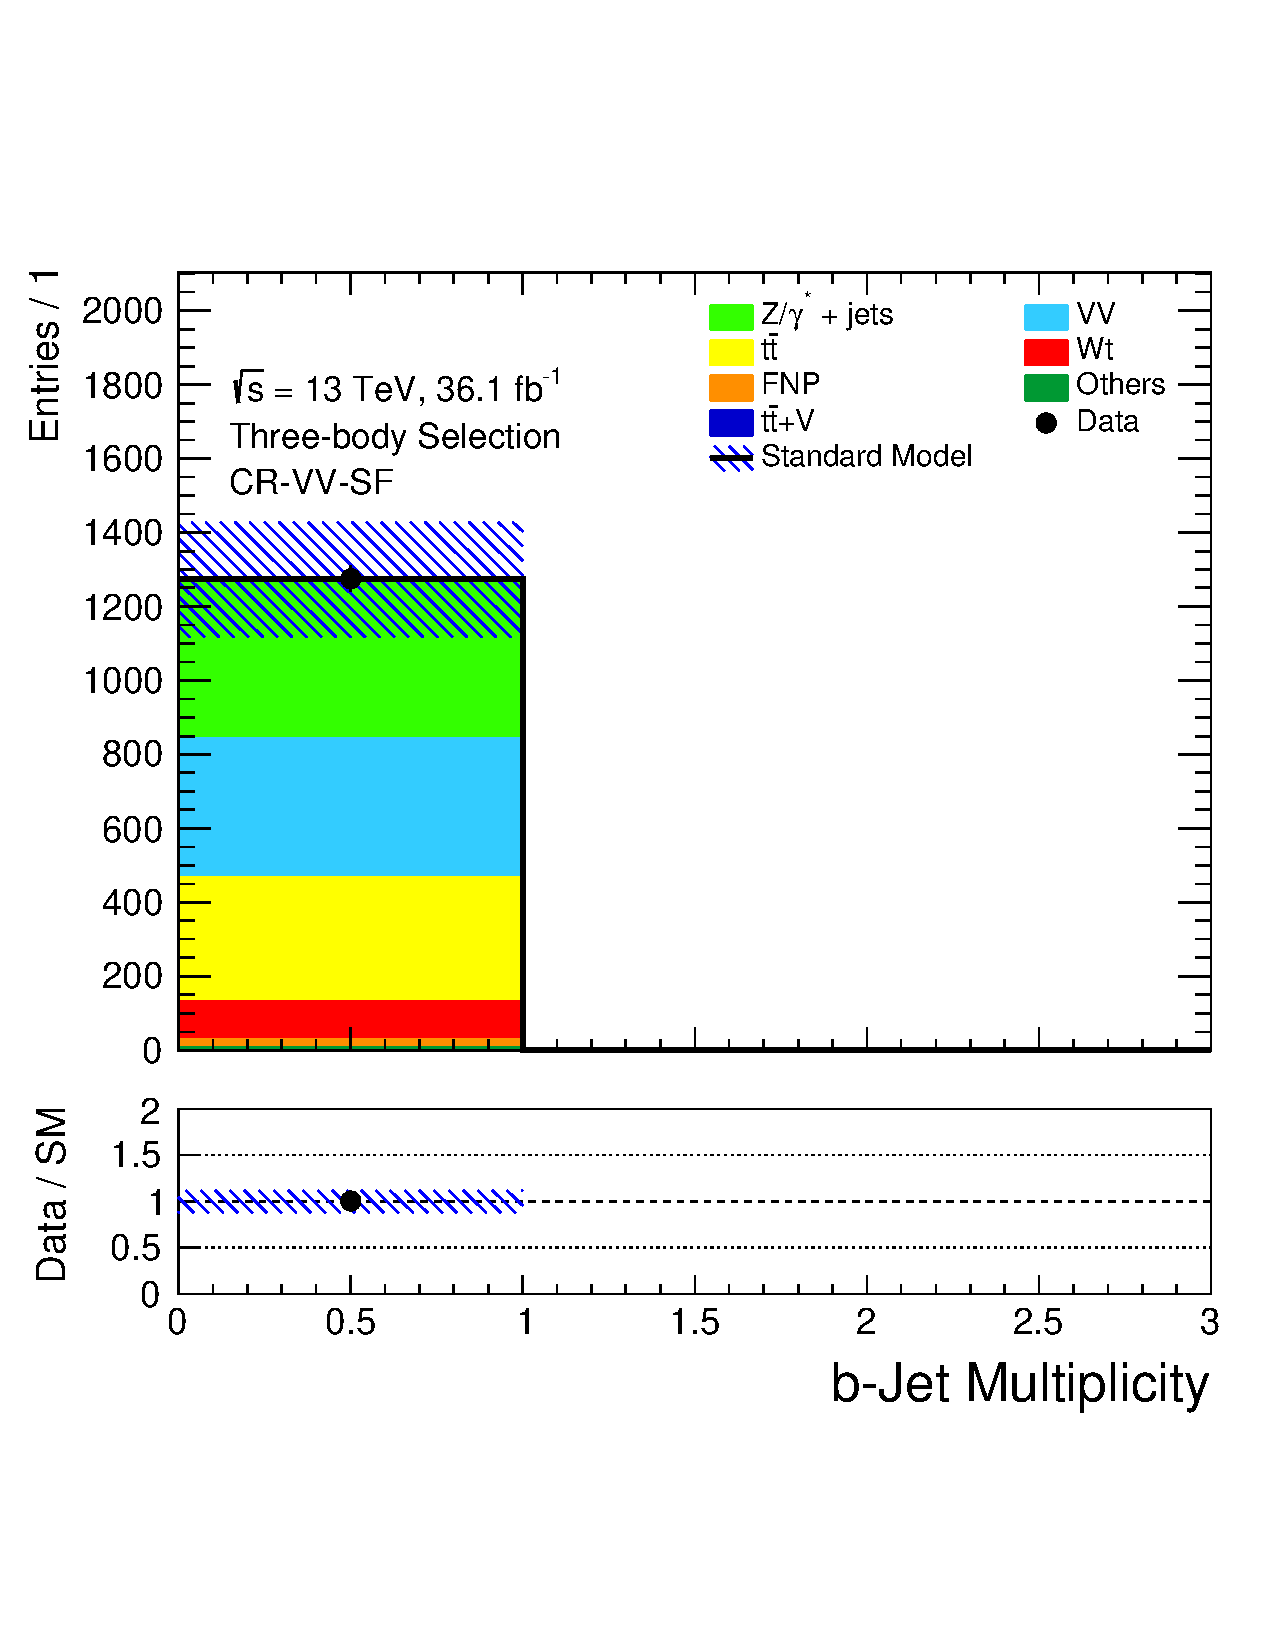
\includegraphics[width=0.48\textwidth]{figures/search_stop2l/bkg_est/crvsf/crvSF_nBJets}
        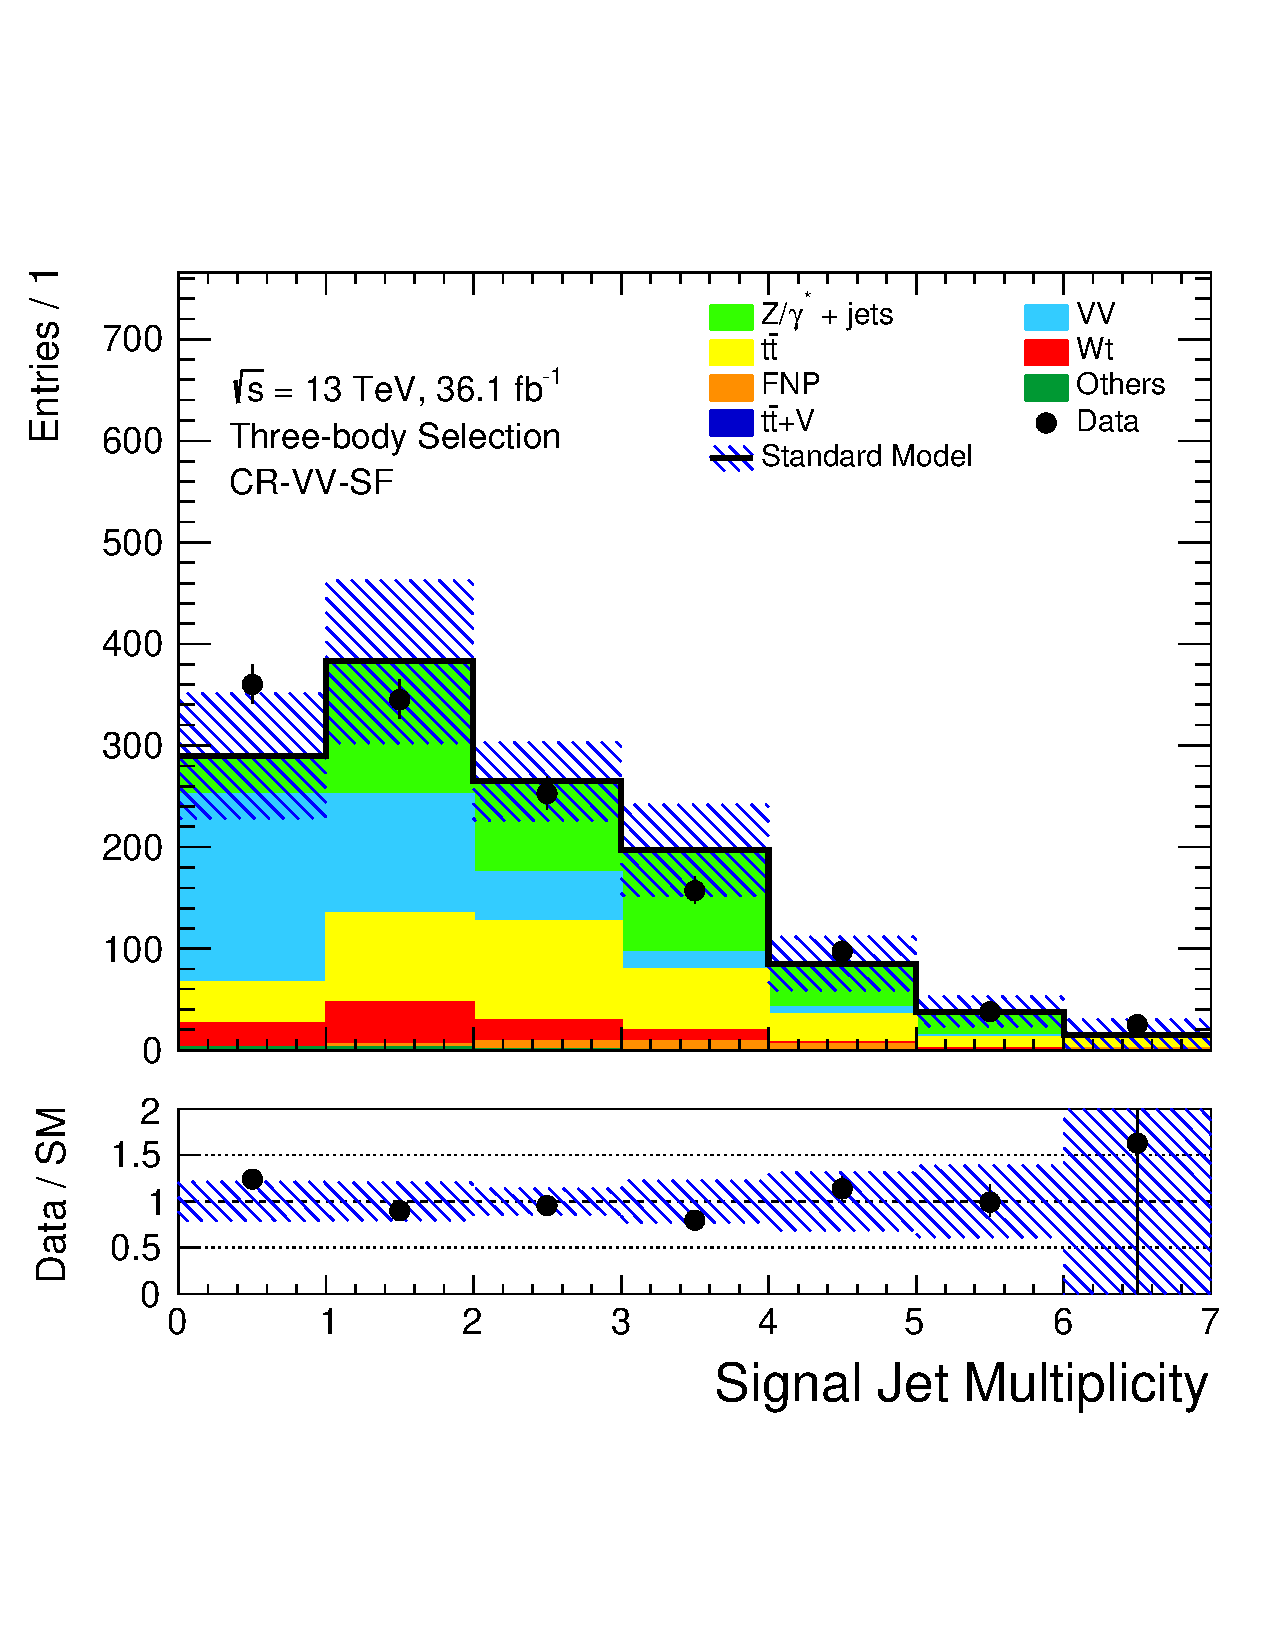
\includegraphics[width=0.48\textwidth]{figures/search_stop2l/bkg_est/crvsf/crvSF_nSJets}
        \caption{
            Distributions of \rpt (\textit{\textbf{upper left}}), leading lepton \gaminv~(\textit{\textbf{upper right}}),
            $b$-tagged jet multiplicity (\textit{\textbf{lower left}}), and non-$b$-tagged jet multiplicity(\textit{\textbf{lower right}}) in the same-flavor diboson CR,
            CR-VV-SF.
            The error on the SM processes includes statistical and systematic uncertainties.
            The post-fit normalization correction factors for the \ttbar and diboson processes
            have been applied.
        }
        \label{fig:crvvSF_1}
    \end{center}
\end{figure}

\begin{figure}[!htb]
    \begin{center}
        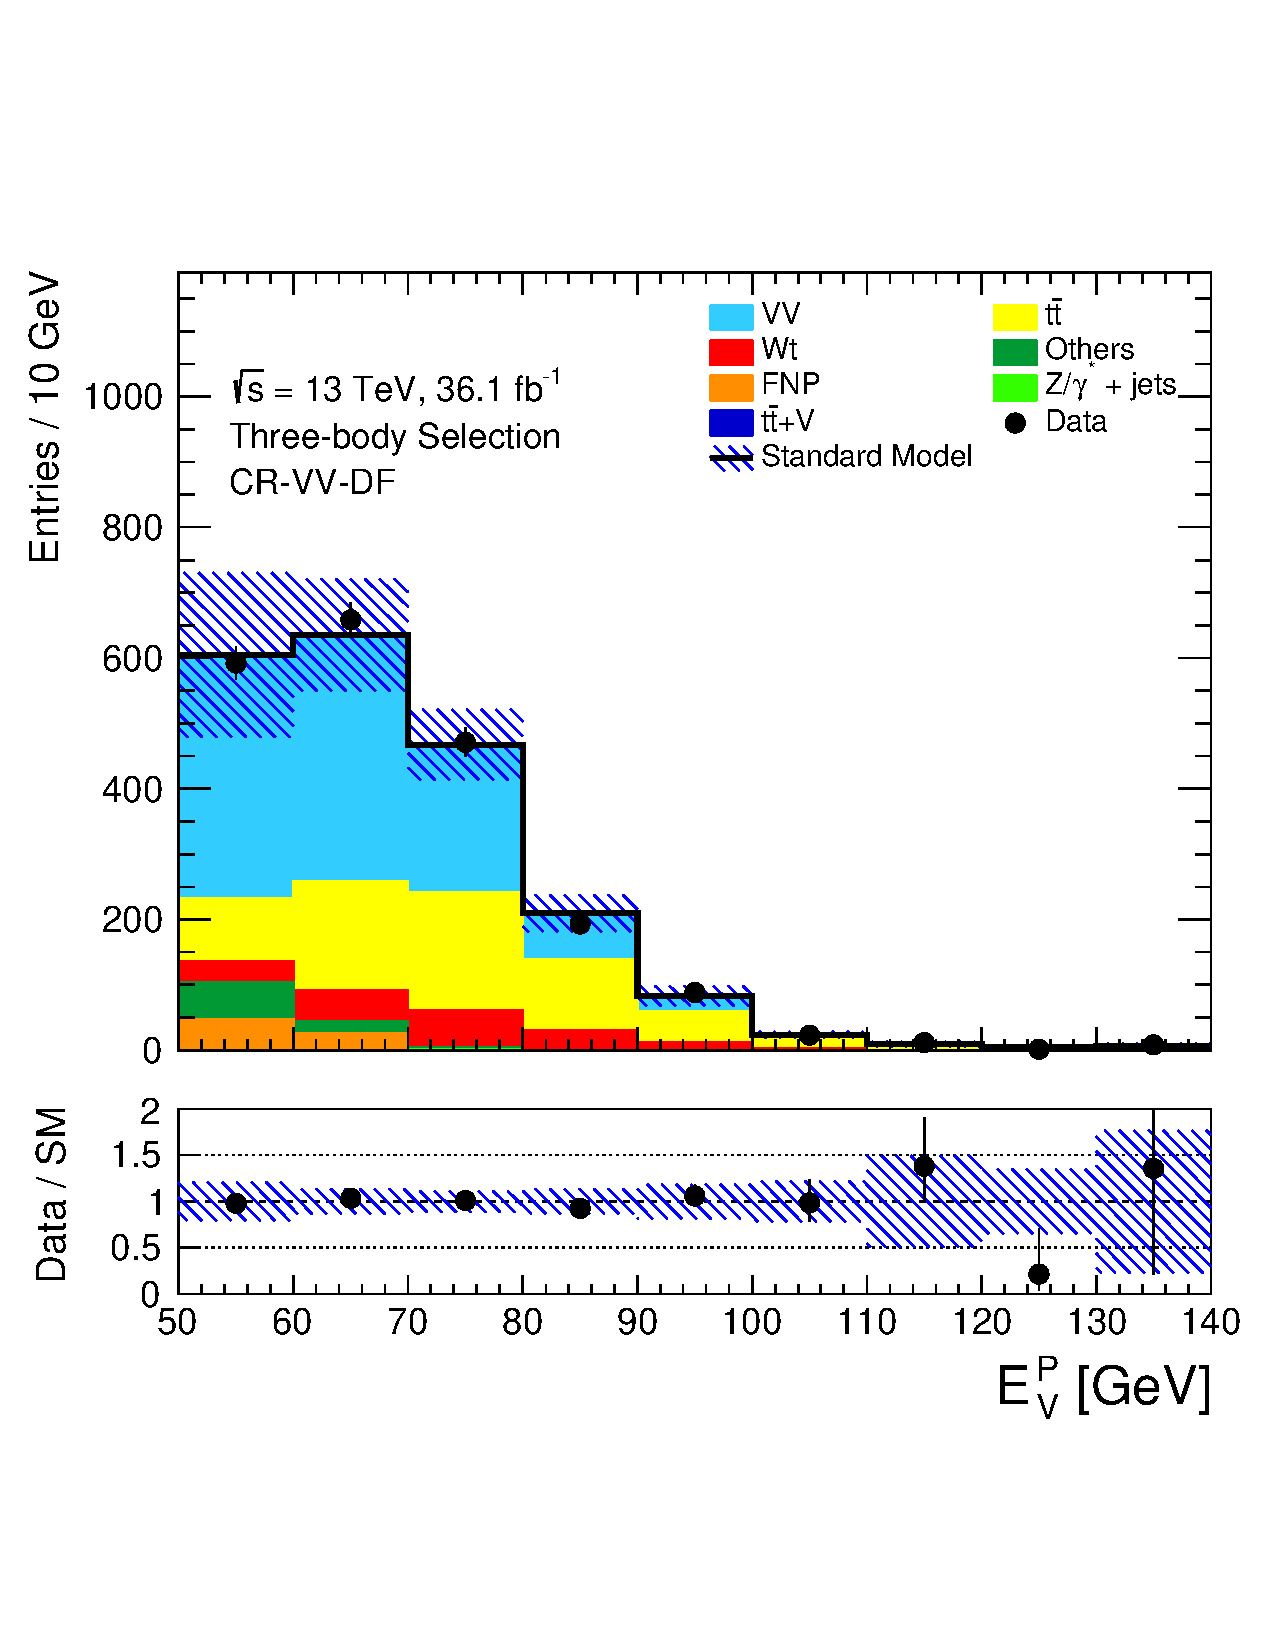
\includegraphics[width=0.48\textwidth]{figures/search_stop2l/bkg_est/crvdf/crv_MDR}
        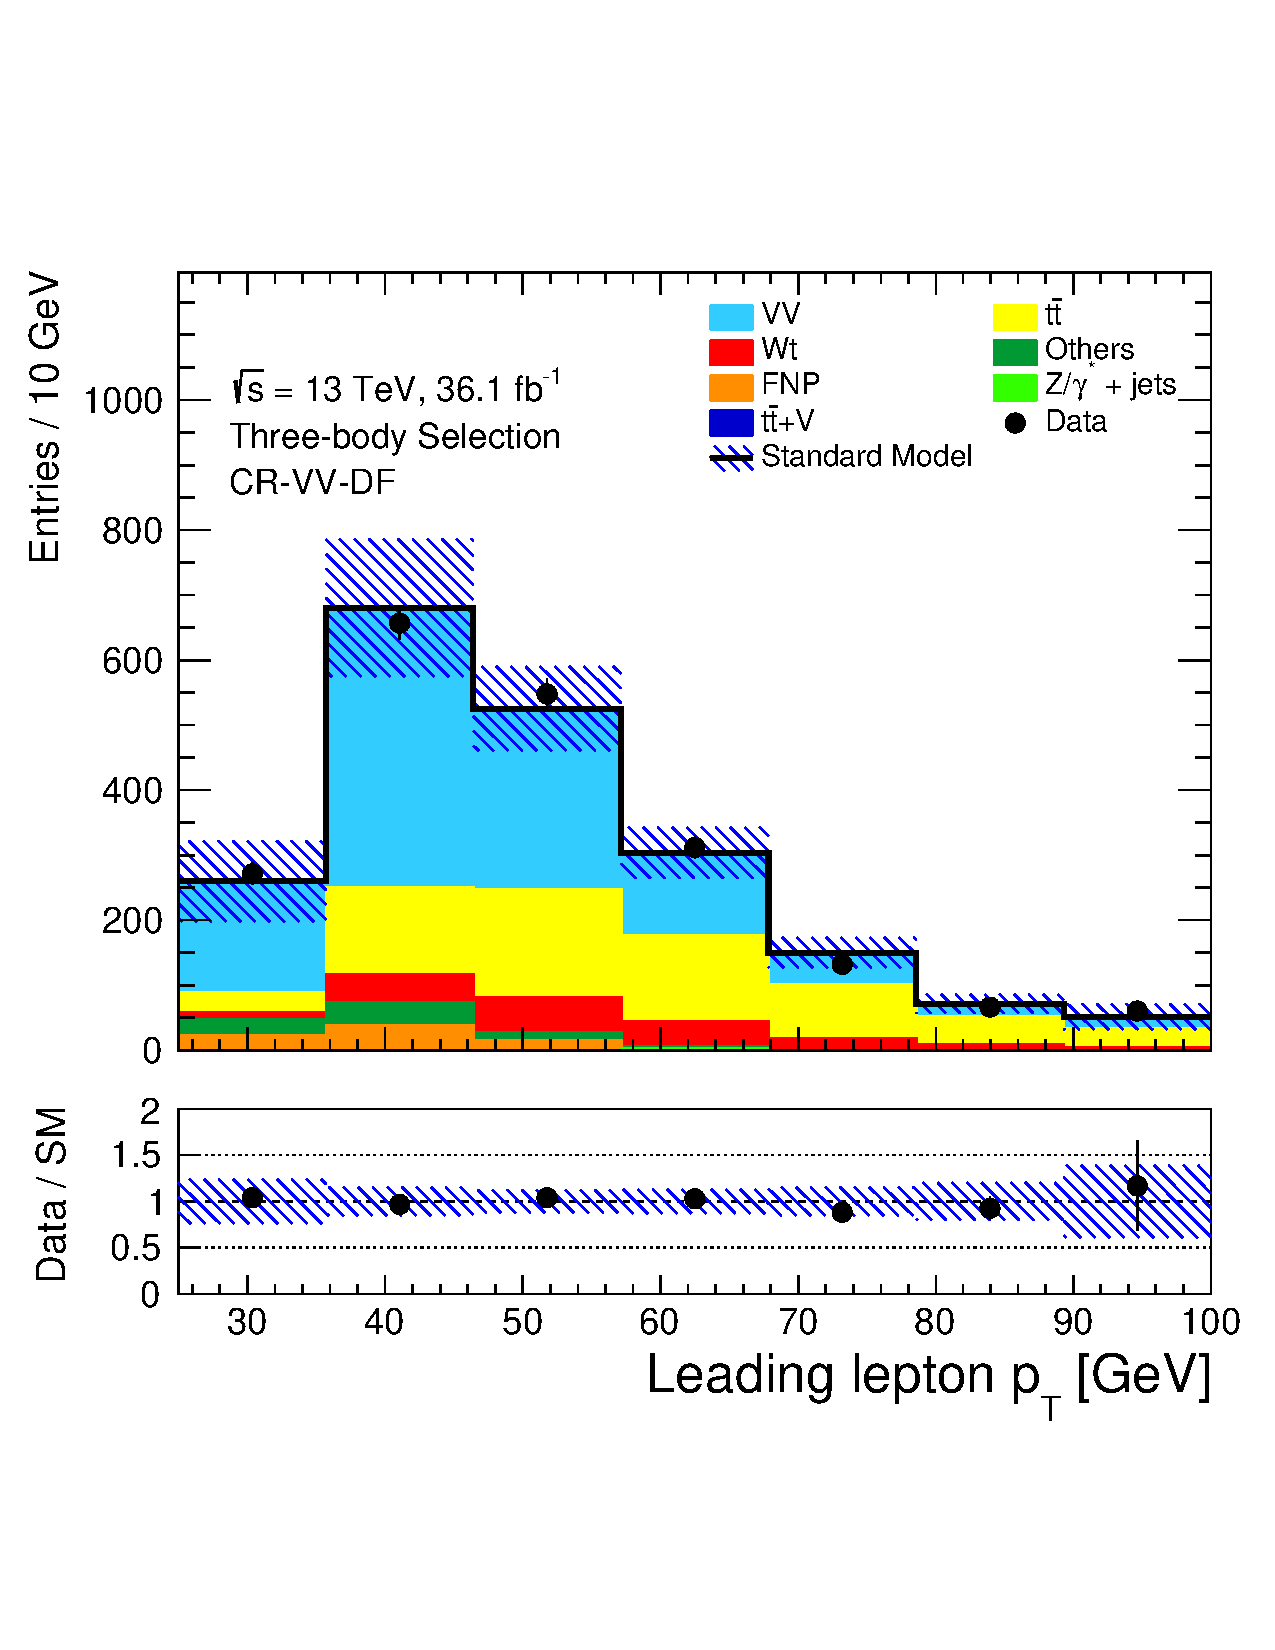
\includegraphics[width=0.48\textwidth]{figures/search_stop2l/bkg_est/crvdf/crv_l_pt0}
        \includegraphics[width=0.48\textwidth]{figures/search_stop2l/bkg_est/crvdf/crv_DPB_vSS}
        \includegraphics[width=0.48\textwidth]{figures/search_stop2l/bkg_est/crvdf/crv_cosThetaB}
        \caption{
            Distributions of \mdr (\textit{\textbf{upper left}}), leading lepton \pT~(\textit{\textbf{upper right}}),
            \dpb (\textit{\textbf{lower left}}), and $|\cosb|$ (\textit{\textbf{lower right}}) in the different-flavor diboson CR,
            CR-VV-DF.
            The error on the SM processes includes statistical and systematic uncertainties.
            The post-fit normalization correction factors for the \ttbar and diboson processes
            have been applied.
        }
        \label{fig:crvvDF_0}
    \end{center}
\end{figure}
\begin{figure}[!htb]
    \begin{center}
        \includegraphics[width=0.48\textwidth]{figures/search_stop2l/bkg_est/crvdf/crv_RPT}
        \includegraphics[width=0.48\textwidth]{figures/search_stop2l/bkg_est/crvdf/crv_gamInvRp1}
        \includegraphics[width=0.48\textwidth]{figures/search_stop2l/bkg_est/crvdf/crv_nBJets}
        \includegraphics[width=0.48\textwidth]{figures/search_stop2l/bkg_est/crvdf/crv_nSJets}
        \caption{
            Distributions of \rpt (\textit{\textbf{upper left}}), leading lepton \gaminv~(\textit{\textbf{upper right}}),
            $b$-tagged jet multiplicity (\textit{\textbf{lower left}}), and non-$b$-tagged jet multiplicity(\textit{\textbf{lower right}}) in the different-flavor diboson CR,
            CR-VV-DF.
            The error on the SM processes includes statistical and systematic uncertainties.
            The post-fit normalization correction factors for the \ttbar and diboson processes
            have been applied.
        }
        \label{fig:crvvDF_1}
    \end{center}
\end{figure}

\FloatBarrier
%%%%%%%%%%%%%%%%%%%%%%%%%%%%%%%%%%%%%%%%%%%%%%%%%%%%%%%%%%%%%%%%%%%%%%%%%%%%%%%%%%%%%%%%%%%%
%%%%%%%%%%%%%%%%%%%%%%%%%%%%%%%%%%%%%%%%%%%%%%%%%%%%%%%%%%%%%%%%%%%%%%%%%%%%%%%%%%%%%%%%%%%%
%%%%%%%%%%%%%%%%%%%%%%%%%%%%%%%%%%%%%%%%%%%%%%%%%%%%%%%%%%%%%%%%%%%%%%%%%%%%%%%%%%%%%%%%%%%%
%
% POST FIT
%
%%%%%%%%%%%%%%%%%%%%%%%%%%%%%%%%%%%%%%%%%%%%%%%%%%%%%%%%%%%%%%%%%%%%%%%%%%%%%%%%%%%%%%%%%%%%
%%%%%%%%%%%%%%%%%%%%%%%%%%%%%%%%%%%%%%%%%%%%%%%%%%%%%%%%%%%%%%%%%%%%%%%%%%%%%%%%%%%%%%%%%%%%
%%%%%%%%%%%%%%%%%%%%%%%%%%%%%%%%%%%%%%%%%%%%%%%%%%%%%%%%%%%%%%%%%%%%%%%%%%%%%%%%%%%%%%%%%%%%

\subsection{Background-only Fit}
\label{sec:stop_background_only}

In order to assess the impact of the CRs on the background estimation in the SRs, a so-called `background-only'
fit is performed.
A background-only fit is profile-likelihood fit, as described Section~\ref{sec:likelihood},
in which the only regions contributing to the likelihood (c.f Equation~\ref{eq:full_likelihood})
are the analysis' CRs.
The result of running a background-only fit to data in the CRs is shown in Table~\ref{tab:bkgonly_CRVR},
which shows the MC predicted yields for the background processes both before and after the
background-only fit is performed, as well as the observed data counts, in each of the CRs and VRs in the analysis.
The post-fit yields in the CRs are expected to agree with the observed data counts, since the latter are used
as constraints in the fit model and there are as many freely-floating parameters in the fit (3 $\mu$ factors)
as there are CRs; therefore, the fit has enough freedom to cover any discrepancy between the observed data and pre-fit MC prediction of
the background processes.
The agreement observed between the post-fit MC and the observed data in the VRs shows that the extrapolation,
at least in terms of the corrected MC's normalisation, is performing well.

The normalisation correction factors for the \ttbar~and diboson processes obtained in the background-only
fit are listed in Table~\ref{tab:stop_scalefactors}.
They are generally consistent with one.

\begin{table}[!htb]
\begin{center}
\setlength{\tabcolsep}{0.0pc}
{\scriptsize
\caption{
Yields in the \ttbar~and diboson CRs and VRs for the \bWN search for the main background processes
contributing to the analysis.
The lower-portion of the table are the yields before the background-only fit to data
in the CRs, without the normalisation corrections applied.
The upper-portion of the table are those taken after the background-only fit to data.
The errors on the quoted numbers are due to the statistical and experimental systematic uncertainties.
}
\label{tab:bkgonly_CRVR}
\begin{tabular*}{\textwidth}{@{\extracolsep{\fill}}lrrrrrr}
\noalign{\smallskip}\hline\noalign{\smallskip}
\noalign{\smallskip}\hline\noalign{\smallskip}
\textbf{Process}           & \textbf{CR-Top}            & \textbf{CR-VV-DF}            & \textbf{CR-VV-SF}            & \textbf{VR-Top}           & \textbf{VR-VV-DF}            & \textbf{VR-VV-SF}              \\[-0.05cm]
\noalign{\smallskip}\hline\noalign{\smallskip}


Observed Data         & $951$              & $2046$              & $1275$              & $1197$              & $1896$              & $783$                    \\
\noalign{\smallskip}\hline\noalign{\smallskip}
%%
Post-fit Total SM         & $951.00 \pm 30.84$          & $2046.05 \pm 45.23$          & $1275.17 \pm 35.68$          & $1231.78 \pm 86.59$          & $2013.57 \pm 116.49$          & $780.44 \pm 117.32$              \\
\noalign{\smallskip}\hline\noalign{\smallskip}
%%
        Post-fit \ttbar          & $833.03 \pm 32.85$          & $619.74 \pm 111.40$          & $333.62 \pm 60.91$          & $733.87 \pm 64.91$          & $754.94 \pm 78.17$          & $127.14 \pm 22.09$              \\
%%
        Post-fit Diboson (DF)          & $11.51 \pm 2.43$          & $1093.28 \pm 125.83$          & $0.00 \pm 0.00$          & $331.13 \pm 82.57$          & $886.53 \pm 168.16$          & $0.00 \pm 0.00$              \\
%%
        Post-fit Diboson (SF)          & $0.00 \pm 0.00$          & $0.00 \pm 0.00$          & $378.94 \pm 124.32$          & $0.00 \pm 0.00$          & $0.00 \pm 0.00$          & $380.00 \pm 141.58$              \\
%%
        Post-fit Single-top          & $101.10 \pm 9.73$          & $186.47 \pm 27.99$          & $103.47 \pm 17.43$          & $111.52 \pm 14.49$          & $151.88 \pm 14.37$          & $36.40 \pm 5.62$              \\
%%
        Post-fit $\ttbar+V$          & $4.35 \pm 0.42$          & $0.39 \pm 0.07$          & $0.36 \pm 0.07$          & $1.27 \pm 0.22$          & $0.42 \pm 0.13$          & $0.05 \pm 0.02$              \\
%%
        Post-fit $Z$+jets          & $0.70 \pm 0.22$          & $1.83_{-1.83}^{+2.55}$          & $428.58 \pm 92.55$          & $0.47_{-0.47}^{+0.85}$          & $0.39_{-0.39}^{+0.71}$          & $191.37 \pm 78.38$              \\
%%
        Post-fit Single-higgs          & $0.31 \pm 0.13$          & $78.95 \pm 9.17$          & $6.23 \pm 1.06$          & $0.44_{-0.44}^{+0.52}$          & $54.98 \pm 4.34$          & $9.40 \pm 1.11$              \\
%%
        Post-fit Fakes          & $0.00 \pm 0.00$          & $65.37 \pm 2.22$          & $23.96 \pm 1.25$          & $53.09 \pm 1.92$          & $164.42 \pm 5.68$          & $36.09 \pm 3.04$              \\
%%
 \noalign{\smallskip}\hline\noalign{\smallskip}
%%
 Total SM               & $905.14 \pm 16.54$          & $1988.38 \pm 110.43$          & $1248.21 \pm 123.42$          & $1184.39 \pm 71.23$          & $1952.92 \pm 61.72$          & $764.65 \pm 99.06$              \\
\noalign{\smallskip}\hline\noalign{\smallskip}
%%
         \ttbar          & $787.43 \pm 11.29$          & $585.87 \pm 102.00$          & $315.39 \pm 55.87$          & $693.71 \pm 53.51$          & $713.64 \pm 66.57$          & $120.19 \pm 20.17$              \\
%%
         Diboson (DF)          & $11.25 \pm 1.62$          & $1069.46 \pm 12.45$          & $0.00 \pm 0.00$          & $323.89 \pm 50.27$          & $867.18 \pm 77.75$          & $0.00 \pm 0.00$              \\
%%
         Diboson (SF)          & $0.00 \pm 0.00$          & $0.00 \pm 0.00$          & $370.13 \pm 15.48$          & $0.00 \pm 0.00$          & $0.00 \pm 0.00$          & $371.16 \pm 34.38$              \\
%%
         Single-top          & $101.10 \pm 9.80$          & $186.49 \pm 28.25$          & $103.49 \pm 17.59$          & $111.52 \pm 14.60$          & $151.88 \pm 14.46$          & $36.41 \pm 5.66$              \\
%%
         $\ttbar+V$          & $4.35 \pm 0.42$          & $0.39 \pm 0.07$          & $0.36 \pm 0.07$          & $1.27 \pm 0.23$          & $0.42 \pm 0.13$          & $0.05 \pm 0.02$              \\
%%
         $Z$+jets          & $0.70 \pm 0.23$          & $1.83_{-1.83}^{+2.57}$          & $428.65 \pm 93.15$          & $0.48_{-0.48}^{+0.86}$          & $0.40_{-0.40}^{+0.72}$          & $191.36 \pm 78.78$              \\
%%
         Single-higgs          & $0.31 \pm 0.13$          & $78.96 \pm 9.26$          & $6.23 \pm 1.07$          & $0.44_{-0.44}^{+0.53}$          & $54.98 \pm 4.37$          & $9.40 \pm 1.12$              \\
%%
         Fakes          & $0.00 \pm 0.00$          & $65.37 \pm 2.23$          & $23.96 \pm 1.26$          & $53.09 \pm 1.92$          & $164.42 \pm 5.70$          & $36.09 \pm 3.04$              \\
\noalign{\smallskip}\hline\noalign{\smallskip}
\noalign{\smallskip}\hline\noalign{\smallskip}
\end{tabular*}
}
\end{center}
\end{table}

\begin{table}[!htb]
    \begin{center}
        \caption{
            Normalisation correction factors for the \ttbar~$(\mu_{\ttbar})$,
            same-flavor diboson $(\mu_{\text{VV-SF}})$, and different-flavor diboson $(\mu_{\text{VV-DF}})$
            processes derived from the background-only fit to the CRs.
            The errors on the quoted numbers are due to the statistical and experimental systematic uncertainties
            entering the fit.
        }
        \label{tab:stop_scalefactors}
        \begin{tabular}{l|c}
            \hline
            \hline
                $\mu_{\ttbar}$ & $1.06 \pm 0.05$ \\
                $\mu_{\text{VV-SF}}$ & $1.02 \pm 0.35$ \\
                $\mu_{\text{VV-DF}}$ & $1.02 \pm 0.12$ \\
            \hline
            \hline
        \end{tabular}
    \end{center}
\end{table}


\section{Results}
\label{sec:hh_results}

As with the analysis presented in Chapter~\ref{chap:search_stop}, a profile likelihood
fit is performed, including all CRs and SRs of the analysis and with the observed
data in all regions used as a constraint.
The result of running this fit is shown in Table~\ref{tab:hh_final_sr_yields}.
The observed data and post-fit MC prediction agrees quite well in SR-SF.
In SR-DF there is a slight excess observed in the data relative to the MC prediction.
This excess in SR-DF is not statistically significant however, and amounts to only a $1.05\sigma$ excess
(null $p_0$-value of 0.15).
Figures~\ref{fig:hh_sr_kin_0}-\ref{fig:hh_sr_kin_3} present kinematic distributions comparing
the observed data and post-fit MC prediction for the SM backgrounds in the SR selections.
Figures~\ref{fig:hh_sr_kin_1} and \ref{fig:hh_sr_kin_2} show the \dhh distributions in detail
in SR-DF and SR-SF, respectively.

As there is no significant deviation between the prediction and observed data,
indicating that there is no evidence for enhanced production of Higgs boson pairs, 95\% CL
cross-section upper-limits are derived for the SM-like non-resonant Higgs boson pair
production.
These results are reported in Table~\ref{tab:hh_bbww_xsec_ul} and are with respect to the
$pp \rightarrow hh$ production process, having taken into account the branching ratio for the dilepton $hh \rightarrow \bbww$
decay.
That is, the 95\% CL UL reported in Table~\ref{tab:hh_bbww_xsec_ul} are on \sigmaHH, and not
on $\sigmaHH \times \text{BR}(hh \rightarrow \bbww) \times \text{BR}(WW^* \rightarrow \ell \nu \ell \nu)$.
The effect of the $1.05\sigma$ excess in SR-DF is seen in the observed 95\% CL UL, which in Table~\ref{tab:hh_bbww_xsec_ul}
is seen to be larger than the expected value by roughly $1\sigma$.
Figure~\ref{fig:hh_ul_comp} illustrates the results listed in Table~\ref{tab:hh_bbww_xsec_ul},
while also comparing them to the leading $hh$ searches (c.f. Figure~\ref{fig:hh_comb_36}): $hh \rightarrow \bbbb$,
$hh \rightarrow \bbtautau$, and $hh \rightarrow \bbyy$.
The comparisons with the other analyses are made only with respect to the expected 95\% CL cross-section upper-limits.
It should be remembered that the other analyses in Figure~\ref{fig:hh_comb_36} are based only on the partial Run 2
dataset, collected in 2015--2016 and comprised of $36.2$\,fb$^{-1}$ of $pp$ collision data.
However, the analysis presented in this chapter is the first time that this search has been performed
in ATLAS and it is already improving the prospects of searches for $hh$ in the \bbww channel by roughly
a factor of 10 (c.f. Figure~\ref{fig:hh_comb_36}).
%At the time of writing, work has already started with the aim of improving the results presented here.
One such improvement, based on performing a multi-binned shape analysis wherein the full \textit{shape} of the \dhh
distribution is used as input to the hypothesis tests --- as opposed to simply \textit{cutting} on the \dhh distribution
and defining simple signal regions as in Table~\ref{tab:hh_sr_def} --- is expected to increase the sensitivity to the $hh \rightarrow \bbww$ signal process
substantially.

One question that the searches for Higgs boson pair production should being thinking about,
as they start preparing for the time when they begin to make observation of Higgs boson pairs,
is whether or not they are designed in such a way as to make meaningful statements about the
Higgs self-coupling parameter, $\lambda$.
As shown in Figure~\ref{fig:hh_feynman}, the leading contributions to Higgs boson pair production
at the LHC proceeds via two diagrams, only one of which is sensitive to $\lambda$.
The final state kinematics resulting from Higgs bosons originating from the decay of the box-diagram
process tend to be much harder due to the massive top-quark loop being directly coupled to the outgoing Higgs bosons.
As a result, analyses are typically more sensitive to this process as the final state objects are
more directly observable and more efficiently reconstructed.
This is the case for the analysis presented in this chapter, a fact that is illustrated in Figure~\ref{fig:mhh_sel_eff}.
The $hh$ system invariant mass in the box-diagram decays
tends to be larger than that of the triangle diagram.
An indication, then, of whether an analysis is tuned to be sensitive to decays relevant
for the measurement of $\lambda$ is whether or not they are sensitive to the lower portion of the $m_{hh}$ distribution.
From Figure~\ref{fig:mhh_sel_eff}, it is clear that the present analysis is more sensitive to the decays from the box-diagram.
Given the early stages of the $hh$ search program in ATLAS, however, this is not currently
an urgent issue.
The preliminary aim for the $hh$ search program has been to define exactly which channels will be effective
at observing $hh$ signal events, in general, and to design analyses that can optimally search
for the many potential sources of \textit{enhanced} Higgs boson pair production.
As the searches become sensitive to the $hh$ production process, as predicted in the SM,
the next steps will be to understand how to design the analyses such that they maximally
discriminate between the box-type and triangle-type kinematics so as to improve the overall prospects
for the measurement of the Higgs self-coupling parameter.

\begin{table}[!htb]
    \begin{center}
        \caption{
            Observed and predicted yields in the SRs for the dilepton $hh \rightarrow \bbww$ search.
        }
        \label{tab:hh_final_sr_yields}
        \begin{tabular}{l | c c}
        \hline
        \hline
                & \multicolumn{2}{c}{\textbf{Regions}} \\
            \cline{2-3}
            \textbf{Process} & \textbf{SR-SF} & \textbf{SR-DF} \\
            \hline
            Observed Data   & 16 & 9 \\
            \hline
            Post-fit Total SM & $14.88 \pm 2.12$ & $4.88 \pm 1.24$ \\
            \hline
            Post-fit \ttbar & $2.57 \pm 0.97$ & $1.74 \pm 0.66$ \\
            Post-fit Single-top $Wt$ & $2.27 \pm 0.54$ & $2.04 \pm 0.64$ \\
            Post-fit $Z$+heavy-flavor & $7.76 \pm 1.04$ & $0.21 \pm 0.05$ \\
            \hline
            SM & $14.12 \pm 2.05$ & $5.83 \pm 1.42$ \\
            \hline
            \ttbar & $3.26 \pm 1.17$ & $2.20 \pm 0.80$ \\
            Single-top $Wt$ & $2.88 \pm 0.59$ & $2.58 \pm 0.75$ \\
            $\ttbar + V$ & $0.59 \pm 0.07$ & $0.07  \pm 0.06$ \\
            $Z$+heavy-flavor & $5.71 \pm 0.74$ & $0.15 \pm 0.04$ \\
            $Z$+light-flavor & $0.32 \pm 0.14$ & $0.00 \pm 0.00$ \\
            Single-higgs & $0.72 \pm 0.09$ & $0.32 \pm 0.06$ \\
            Fakes & $0.54 \pm 0.38$ & $0.42 \pm 0.36$ \\
        \hline
        \hline
        \end{tabular}
    \end{center}
\end{table}

\begin{table}[!htb]
    \begin{center}
        \caption{
            Expected and observed 95\% CL upper-limits on the Standard Model, non-resonant $hh$
            production cross-section ($\sigma(pp \rightarrow hh)$) and on
            the ratio of the upper-limit on this value to the value predicted in the SM
            ($\sigmaSM = 31.05$ fb).
            The observed limits are in the right most column.
            The $\pm 1 \sigma$ and $\pm 2\sigma$ excursions from the median expected value incorporate the
            effects of the analysis' systematic uncertainties.
        }
        \label{tab:hh_bbww_xsec_ul}
        \begin{tabular}{l | c | c | c | c | c || c }
            \hline
            \hline
                    & $-2\sigma$ & $-1 \sigma$ & \textbf{Median Expected} & $+1 \sigma$ & $+2 \sigma$ & \textbf{Observed} \\
            \hline
                95\% CL UL $\sigma (pp \rightarrow hh)$ [pb] & $0.465$ & $0.641$ & $0.920$ & $1.363$ & $1.990$ & $1.290$ \\
                \sigmaRatio & $14.97$ & $20.66$ & $29.63$ & $43.89$ & $64.02$ & $41.54$ \\
            \hline
            \hline
        \end{tabular}
    \end{center}
\end{table}

%%%%%%%%%%%%%%%%%%%%%%%%%%%%%%%%%%%%%%%%%%%%%%%%%%%%%%%%%%%%%%%%%%%%%%%%%%%%%%%%%%%%%%%%%%%%
%%%%%%%%%%%%%%%%%%%%%%%%%%%%%%%%%%%%%%%%%%%%%%%%%%%%%%%%%%%%%%%%%%%%%%%%%%%%%%%%%%%%%%%%%%%%
%%%%%%%%%%%%%%%%%%%%%%%%%%%%%%%%%%%%%%%%%%%%%%%%%%%%%%%%%%%%%%%%%%%%%%%%%%%%%%%%%%%%%%%%%%%%
%
% SR KIN PLOTS
%
%%%%%%%%%%%%%%%%%%%%%%%%%%%%%%%%%%%%%%%%%%%%%%%%%%%%%%%%%%%%%%%%%%%%%%%%%%%%%%%%%%%%%%%%%%%%
%%%%%%%%%%%%%%%%%%%%%%%%%%%%%%%%%%%%%%%%%%%%%%%%%%%%%%%%%%%%%%%%%%%%%%%%%%%%%%%%%%%%%%%%%%%%
%%%%%%%%%%%%%%%%%%%%%%%%%%%%%%%%%%%%%%%%%%%%%%%%%%%%%%%%%%%%%%%%%%%%%%%%%%%%%%%%%%%%%%%%%%%%

\begin{figure}[!htb]
    \begin{center}
        \includegraphics[width=0.48\textwidth]{figures/search_hh/results/sr_plots/srIncNoMllDhh_mll}
        \includegraphics[width=0.48\textwidth]{figures/search_hh/results/sr_plots/srIncNoMbbDhh_mbb}
        \includegraphics[width=0.48\textwidth]{figures/search_hh/results/sr_plots/srIncNoDhh_NN_d_hh}
        \caption{
            Distributions of $m_{\ell \ell}$ (\textit{\textbf{left}}), $m_{bb}$ (\textit{\textbf{right}}),
            and \dhh (\textit{\textbf{bottom}}).
            The distributions are shown after the fit to data in the control regions under the background-only hypothesis.
            Each distribution includes both the SF and DF events and imposes the analysis SR requirements
            on all quantities except for the one being plotted.
            The SR requirement on \dhh in the $m_{\ell\ell}$ and $m_{bb}$ distributions is relaxed to $\dhh > 5$.
            The dilepton $hh \rightarrow \bbww$ signal, labeled as `$HH$', is shown with its cross-section scaled
            by a factor of 20 relative to the SM prediction for visualization purposes.
            The ratio of the data to the sum of the backgrounds is shown in the lower panel of each figure.
            The hatched bands indicate the combined statistical and systematic uncertainty.
        }
        \label{fig:hh_sr_kin_0}
    \end{center}
\end{figure}

\begin{figure}[!htb]
    \begin{center}
        \includegraphics[width=0.48\textwidth]{figures/search_hh/results/sr_plots/srDFNoDhh_NN_d_hh}
        \includegraphics[width=0.48\textwidth]{figures/search_hh/results/sr_plots/srDFNoDhhCloseCut_NN_d_hh}
        \caption{
            Distributions of the \dhh observable in SR-DF without the \dhh selection applied (\textit{\textbf{left}})
            and with the \dhh selection ($\dhh > 5.55$) applied (\textit{\textbf{right}}).
            The dilepton $hh \rightarrow \bbww$ signal, labeled as `$HH$', is shown with its cross-section scaled
            by a factor of 20 relative to the SM prediction for visualization purposes.
            The ratio of the data to the sum of the backgrounds is shown in the lower panel of each figure.
            The hatched bands indicate the combined statistical and systematic uncertainty.
        }
        \label{fig:hh_sr_kin_1}
    \end{center}
\end{figure}
\begin{figure}[!htb]
    \begin{center}
        \includegraphics[width=0.48\textwidth]{figures/search_hh/results/sr_plots/srSFNoDhh_NN_d_hh}
        \includegraphics[width=0.48\textwidth]{figures/search_hh/results/sr_plots/srSFNoDhhCloseCut_NN_d_hh}
        \caption{
            Distributions of the \dhh observable in SR-SF without the \dhh selection applied (\textit{\textbf{left}})
            and with the \dhh selection ($\dhh > 5.45$) applied (\textit{\textbf{right}}).
            The dilepton $hh \rightarrow \bbww$ signal, labeled as `$HH$', is shown with its cross-section scaled
            by a factor of 20 relative to the SM prediction for visualization purposes.
            The ratio of the data to the sum of the backgrounds is shown in the lower panel of each figure.
            The hatched bands indicate the combined statistical and systematic uncertainty.
        }
        \label{fig:hh_sr_kin_2}
    \end{center}
\end{figure}

\begin{figure}[!htb]
    \begin{center}
        \includegraphics[width=0.48\textwidth]{figures/search_hh/results/sr_plots/srIncNoDhh_dphi_ll}
        \includegraphics[width=0.48\textwidth]{figures/search_hh/results/sr_plots/srIncNoDhh_dRll}
        \caption{
            Distributions of the $|\dphill|$ and $\drll$ quantities in the analysis' SR selections,
            inclusive of SF and DF dilepton flavors and without the \dhh requirements.
            The dilepton $hh \rightarrow \bbww$ signal, labeled as `$HH$', is shown with its cross-section scaled
            by a factor of 20 relative to the SM prediction for visualization purposes.
            The ratio of the data to the sum of the backgrounds is shown in the lower panel of each figure.
            The hatched bands indicate the combined statistical and systematic uncertainty.
        }
        \label{fig:hh_sr_kin_3}
    \end{center}
\end{figure}

\begin{figure}[!htb]
    \begin{center}
        \includegraphics[width=0.6\textwidth]{figures/search_hh/results/hh_ul_compPDF}
        \caption{
            Summary plot showing the $hh$ production cross-section upper limit results, normalized to
            the SM prediction of 31.05\,fb, for the analysis presented in this thesis in green,
            based on the full Run 2 dataset of 139\,fb$^{-1}$ of $pp$ collision data.
            In grey, the partial Run 2 results based on 36\,fb$^{-1}$ of data are shown for comparison.
            Only the expected upper limits are shown.
        }
        \label{fig:hh_ul_comp}
    \end{center}
\end{figure}

\begin{figure}[!htb]
    \begin{center}
        \includegraphics[width=0.6\textwidth]{figures/search_hh/mhh_sel_eff_nice_jul30}
        \caption{
            Analysis selection efficiency for the dilepton $hh \rightarrow \bbww$ signal process
            as a function of the truth-level $hh$ system invariant mass, $m_{HH}$.
            Each color indicates an additional selection applied sequentially, and in the order indicated
            in the legend, with respect to the starting sample of events satisfying the
            analysis' preselection requirements and having at least two $b$-tagged jets.
            For reference, overlaid in grey color, and with arbitrary normalisation, is the truth-level
            $m_{HH}$ distribution.
        }
        \label{fig:mhh_sel_eff}
    \end{center}
\end{figure}

In addition to the 95\% CL cross-section UL reported in Table~\ref{tab:hh_bbww_xsec_ul}, we also perform
a scan over the Higgs self-coupling parameter, $\lambda$, employed in the dilepton $hh \rightarrow \bbww$ signal MC sample
so that we may re-run the analysis for various non-SM hypotheses for the value of $\lambda$.
The variations in the Higgs self-coupling are parametrized by $\kappa_{\lambda} = \lambda / \lambda_{SM}$, and this
value is scanned across the values $\kappa_{\lambda} \in [-20, 20]$.
Changing the value of $\kappa_{\lambda}$ changes the relative strength of the competing triangle
and box diagrams that lead to $hh$ production at LO at the LHC, with only the former sensitive to
the Higgs self-coupling parameter.
Variations in $\kappa_{\lambda}$ can therefore lead to either the box diagram or the triangle diagram being the dominant source of Higgs boson pairs.
This has visible consequences for the final state.
The Higgs bosons from the box diagram tend to have harder transverse momenta
as compared to those from the triangle diagram, for example.
The Higgs bosons from predominantly box diagram production scenarios, then, lead to harder visible final state objects
and a different acceptance to the $hh$ signal as compared to the case in which the Higgs bosons arise predominantly
from the triangle diagram.
Further discussion about the effects of varying $\kappa_{\lambda}$ on the Higgs bosons' kinematics can
be found in Ref.~\cite{HHComb36}.
It should be stressed, however, that the present analysis is in no way optimized for non-SM values of $\kappa_{\lambda}$.
For each new value of this parameter we simply perform the hypothesis tests using the same
sets of SRs and CRs described in the sections above.

The results of the $\kappa_{\lambda}$ scan are shown in Figure~\ref{fig:hh_lambda_scan}.
It can be seen that the anaysis has little constraining power on the Higgs self-coupling parameter, with
the NLO theory prediction for alternative $\kappa_{\lambda}$ hypotheses described in the figure caption.
The lack of ability to more powerfully exclude non-SM values of $\kappa_{\lambda}$ lies in the
fact that the analysis is optimized for the SM case, in particular.
This is illustrated in Figure~\ref{fig:dhh_vs_lambda}, showing the change in \dhh as a function
of $\kappa_{\lambda}$.
It can be seen that large values of \dhh are observed only for those $\kappa_{\lambda}$ values near
the SM hypothesis with $\kappa_{\lambda} \approx 1$.
As a result of the harsh selections (cuts) made on \dhh in SR-SF and SR-DF (c.f. Table~\ref{tab:hh_sr_def}),
sensitivity is lost for essentially all signal hypotheses with non-SM values of $\kappa_{\lambda}$.
Again, this is a result of the analysis having been optimized with only the SM hypothesis in mind.
Future versions of this analysis will hopefully improve the sensitivity to non-SM values of $\kappa_{\lambda}$
such that this parameter may be constrained and, at some point, measured precisely.

One such avenue for improving the analysis' sensitivity to alternative $\kappa_{\lambda}$ hypotheses would be
to inject knowledge of $\kappa_{\lambda}$ into the neural network training, perhaps using
the technique of parametrized machine learning~\cite{Baldi:2016fzo}.
The brute force method, of course, to which the methods described in Ref.~\cite{Baldi:2016fzo} provide an alternative, would be to construct a set of classifiers (potentially many) --- each trained using $hh \rightarrow \bbww$ signal hypotheses with differing values of $\kappa_{\lambda}$ ---
and then assess the sensitivity to specific values of $\kappa_{\lambda}$ hypotheses using
the classifier that has been trained using the $hh$ signal with that value for its Higgs self-coupling parameter.

\begin{figure}[!htb]
    \begin{center}
        \includegraphics[width=0.6\textwidth]{figures/search_hh/results/wwbb_lambda_scan_may7}
        \caption{
            Expected and observed cross-section upper-limit for the dilepton $hh \rightarrow \bbww$ search
            as a function of the Higgs self-coupling parameter, $\kappa_{\lambda} = \lambda_{hhh} / \lambda_{hhh}^{\text{SM}}$.
            The vertical dashed line indicates the SM scenario with $\kappa_{\lambda} = 1$.
            The $\pm 1\sigma$ and $\pm 2 \sigma$ uncertainty band on the expected upper-limit includes the effects
            of all experimental and modelling systematic uncertainties.
            The NLO theory prediction is taken from Ref.~\cite{deFlorian:2016spz} and described fully
            in Ref.~\cite{HHComb36}.
        }
        \label{fig:hh_lambda_scan}
    \end{center}
\end{figure}

\begin{figure}[!htb]
    \begin{center}
        \includegraphics[width=0.6\textwidth]{figures/search_hh/results/dhh_vs_lambda}
        \caption{
            The \dhh distribution as a function of the Higgs self-coupling parameter, $\kappa_{\lambda} = \lambda_{hhh} / \lambda_{hhh}^{\text{SM}}$.
            The trend of the \dhh distribution as a function of $\kappa_{\lambda}$ is directly related to the analysis'
            acceptance to the dilepton $hh \rightarrow \bbww$ signal under non-SM values of $\kappa_{\lambda}$,
            illustrated in Figure~\ref{fig:hh_lambda_scan}.
            The darker the blue color means a higher population of the dilepton $hh \rightarrow \bbww$ signal process.
            The color white indicates that a given region is not populated at all.
        }
        \label{fig:dhh_vs_lambda}
    \end{center}
\end{figure}


